\input{../style/preamble}
\input{../latex-math/basic-math}
\input{../latex-math/basic-ml}
\input{../latex-math/ml-nn}

% Macros and packages the DL4NLP source decks get from their own preamble
% (lecture_dl4nlp/style/preamble_new.tex) or per-file preambles.
\usepackage{animate}
% The course's typewriter font (laett, set in dhbw-lecture.sty) has no bold shape;
% DL4NLP uses \textbf{\texttt{...}}, so map bold typewriter to regular.
\AtBeginDocument{{\ttfamily\selectfont}\DeclareFontShape{T1}{laett}{bx}{n}{<->ssub*laett/m/n}{}\DeclareFontShape{T1}{laett}{m}{bx}{<->ssub*laett/m/n}{}}
\newcommand{\citebutton}[2]{\beamergotobutton{\href{#2}{#1}}}
\newcommand{\ques}{\textbf{\textcolor{red}{Question:  }}}
\definecolor{texblue}{rgb}{0, 0, 1}
\def\myblue#1{\textcolor{texblue}{#1}}
\newcommand{\blu}[1]{\textcolor{blue}{#1}}
\newcommand{\org}[1]{\textcolor{orange}{#1}}
\long\def\devour#1{}
\newcommand\warning{%
 \makebox[1.4em][c]{%
 \makebox[0pt][c]{\raisebox{.1em}{\scriptsize!}}%
 \makebox[0pt][c]{\color{red}\normalsize$\bigtriangleup$}}}%

\newcommand{\titlefigure}{figure/bert-input.png}
\newcommand{\learninggoals}{
  \item Autoregressive vs.\ masked language modeling, and how to measure LM performance
  \item BERT: architecture, pre-training (MLM, NSP), and fine-tuning
  \item Transfer learning and self-supervision
  \item BERTology and the BERT-based family: RoBERTa, ALBERT, DistilBERT
  \item Post-BERT objectives (ELECTRA, XLNet) and T5's text-to-text framing
}

\title{Advanced Artificial Intelligence and Machine Learning}
\date{}

\begin{document}

\lecturechapter{Transformer Architecture Variants: BERT \& T5}
\lecture{Advanced AI \& ML}

%%%%%%%%%%%%%%%%%%%%%%%%%%%%%%%%%%%%%%%%%%%%%%%%%%%%%%%%%%%%%%%%%%
\section{ARLMs vs. MLM}
% Source: DL4NLP chapter04-bert/slides-41-arlm-mlm.tex
%%%%%%%%%%%%%%%%%%%%%%%%%%%%%%%%%%%%%%%%%%%%%%%%%%%%%%%%%%%%%%%%%%
% ------------------------------------------------------------------------------

\begin{frame}{again: what is a language model?}

\vfill

\begin{itemize}
	\item Statistical model that predicts text that fits well for a given context (typically also text)
	\item Auto-regressive LMs (ARLMs)
	\begin{itemize}
		\item Predict one word that is highly likely given a prompt (previous words)
		\item For predicting an entire text, repeat the process (i.e., extend the prompt with previously predicted words)
		\item To predict a text from scratch, use an extra symbol \texttt{<START>} as the initial prompt
	\end{itemize}
\end{itemize}

\vfill

\end{frame}

% ------------------------------------------------------------------------------

\begin{frame}{arlm: toy example}
	\vfill
	\begin{figure}
		\centering
		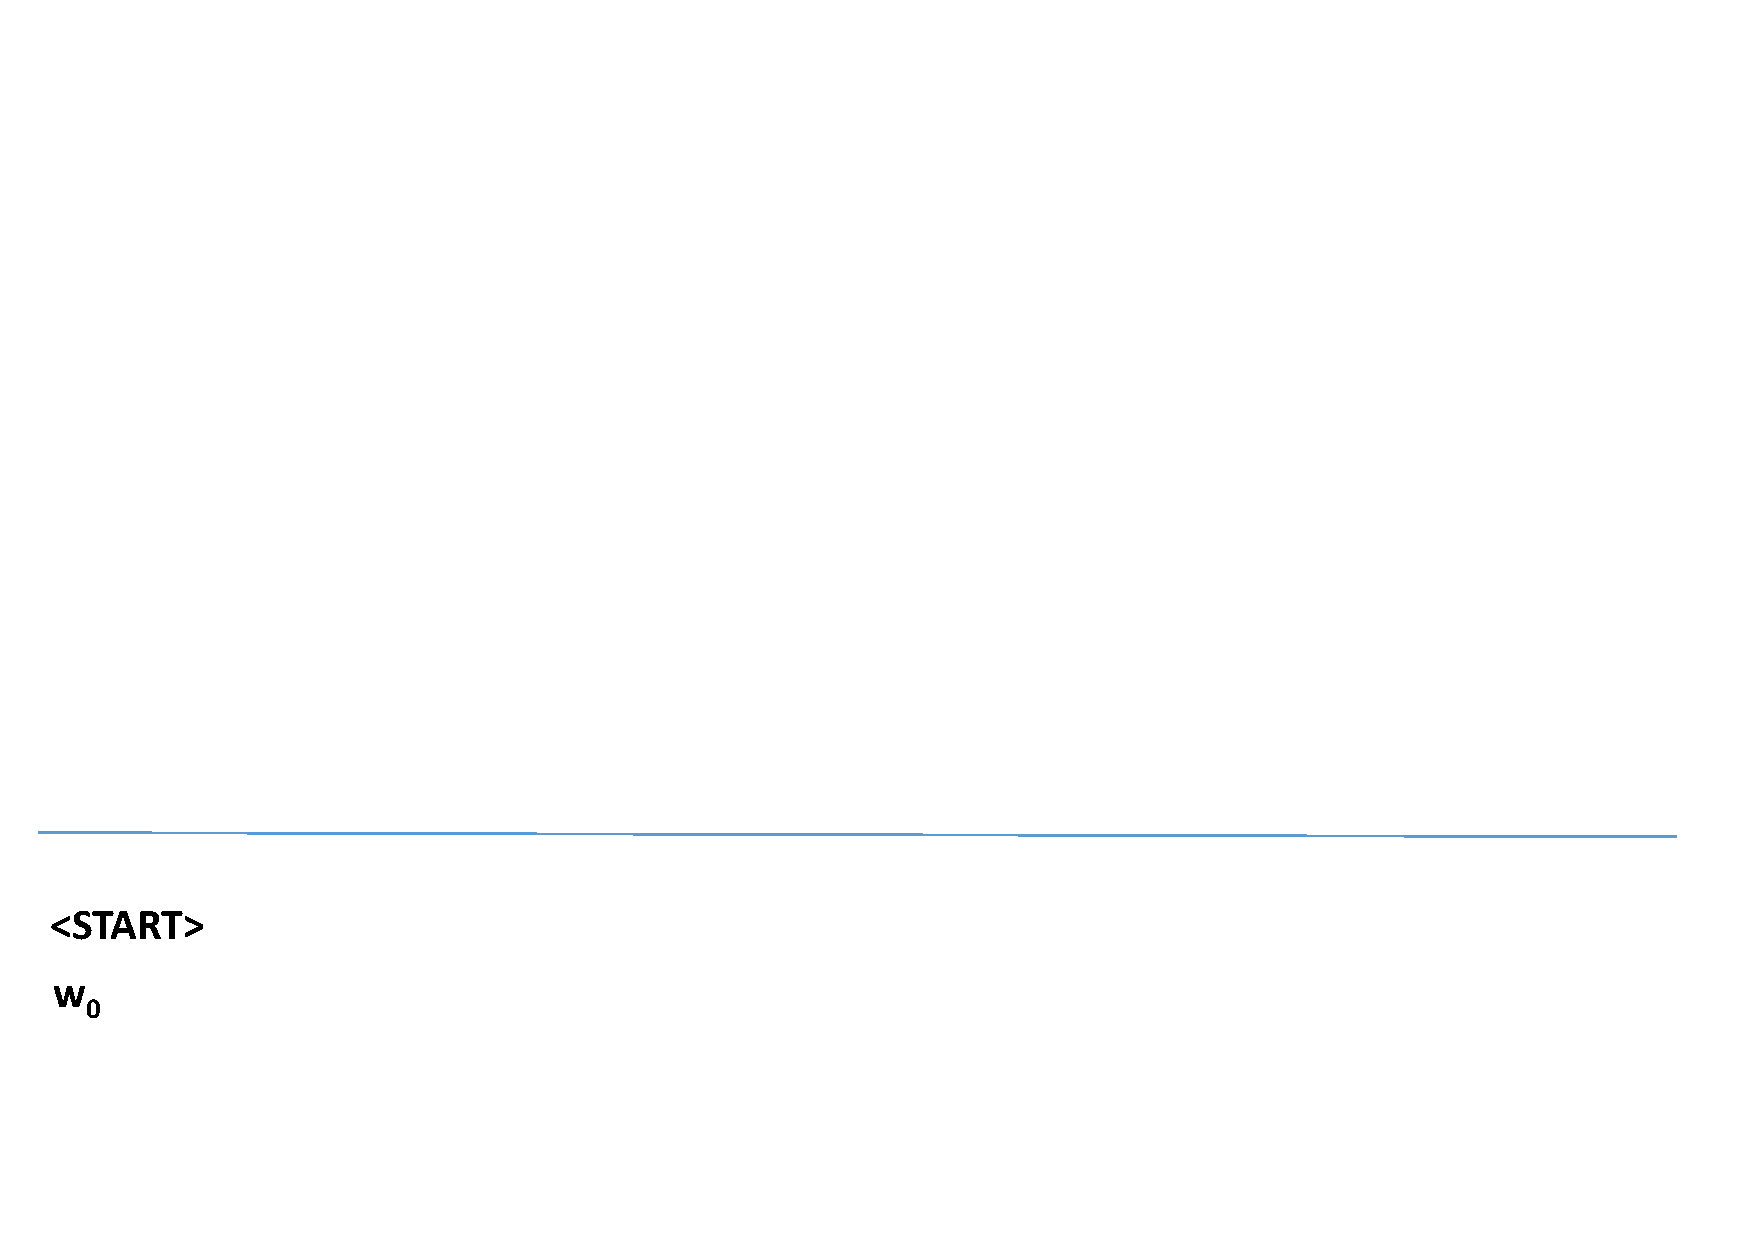
\includegraphics[width=8.67cm,page=1]{figure/arlm.pdf}
	\end{figure}
	\vfill
\end{frame}
\begin{frame}[noframenumbering]{arlm: toy example}
	\vfill
	\begin{figure}
		\centering
		\includegraphics[width=8.67cm,page=2]{figure/arlm.pdf}
	\end{figure}
	\vfill
\end{frame}
\begin{frame}[noframenumbering]{arlm: toy example}
	\vfill
	\begin{figure}
		\centering
		\includegraphics[width=8.67cm,page=3]{figure/arlm.pdf}
	\end{figure}
	\vfill
\end{frame}
\begin{frame}[noframenumbering]{arlm: toy example}
	\vfill
	\begin{figure}
		\centering
		\includegraphics[width=8.67cm,page=4]{figure/arlm.pdf}
	\end{figure}
	\vfill
\end{frame}
\begin{frame}[noframenumbering]{arlm: toy example}
	\vfill
	\begin{figure}
		\centering
		\includegraphics[width=8.67cm,page=5]{figure/arlm.pdf}
	\end{figure}
	\vfill
\end{frame}
\begin{frame}[noframenumbering]{arlm: toy example}
	\vfill
	\begin{figure}
		\centering
		\includegraphics[width=8.67cm,page=6]{figure/arlm.pdf}
	\end{figure}
	\vfill
\end{frame}
\begin{frame}[noframenumbering]{arlm: toy example}
	\vfill
	\begin{figure}
		\centering
		\includegraphics[width=8.67cm,page=7]{figure/arlm.pdf}
	\end{figure}
	\vfill
\end{frame}
\begin{frame}[noframenumbering]{arlm: toy example}
	\vfill
	\begin{figure}
		\centering
		\includegraphics[width=8.67cm,page=8]{figure/arlm.pdf}
	\end{figure}
	\vfill
\end{frame}
\begin{frame}[noframenumbering]{arlm: toy example}
	\vfill
	\begin{figure}
		\centering
		\includegraphics[width=8.67cm,page=9]{figure/arlm.pdf}
	\end{figure}
	\vfill
\end{frame}
\begin{frame}[noframenumbering]{arlm: toy example}
	\vfill
	\begin{figure}
		\centering
		\includegraphics[width=8.67cm,page=10]{figure/arlm.pdf}
	\end{figure}
	\vfill
\end{frame}
\begin{frame}[noframenumbering]{arlm: toy example}
	\vfill
	\begin{figure}
		\centering
		\includegraphics[width=8.67cm,page=11]{figure/arlm.pdf}
	\end{figure}
	\vfill
\end{frame}
\begin{frame}[noframenumbering]{arlm: toy example}
	\vfill
	\begin{figure}
		\centering
		\includegraphics[width=8.67cm,page=12]{figure/arlm.pdf}
	\end{figure}
	\vfill
\end{frame}
\begin{frame}[noframenumbering]{arlm: toy example}
	\vfill
	
	\begin{figure}
		\centering
		\includegraphics[width=8.67cm,page=13]{figure/arlm.pdf}
	\end{figure}
	
	\vfill
\end{frame}

% ------------------------------------------------------------------------------

\begin{frame}{arlm: probabilistic interpretation}

\vfill

\begin{itemize}
	\item Gives an estimate for the probability of a sentence using conditional probabilities
	\item In general: $$ P(A \cap B) = P(B) \cdot P(A | B)$$
	\item For $P(sentence)$:
	$$ P(w_1, w_2, \dots, w_n | w_0)$$ $$ = P(w_1 | w_0) \cdot P(w_2 | w_0, w_1) \cdot \hdots \cdot P(w_n | w_0, \dots, w_{n-1})$$
\end{itemize}

\vfill

\end{frame}

% ------------------------------------------------------------------------------

\begin{frame}{Examples of ARLMs (1)}

\vfill

\textbf{Neural Machine Translation:}

	\begin{figure}
		\centering
		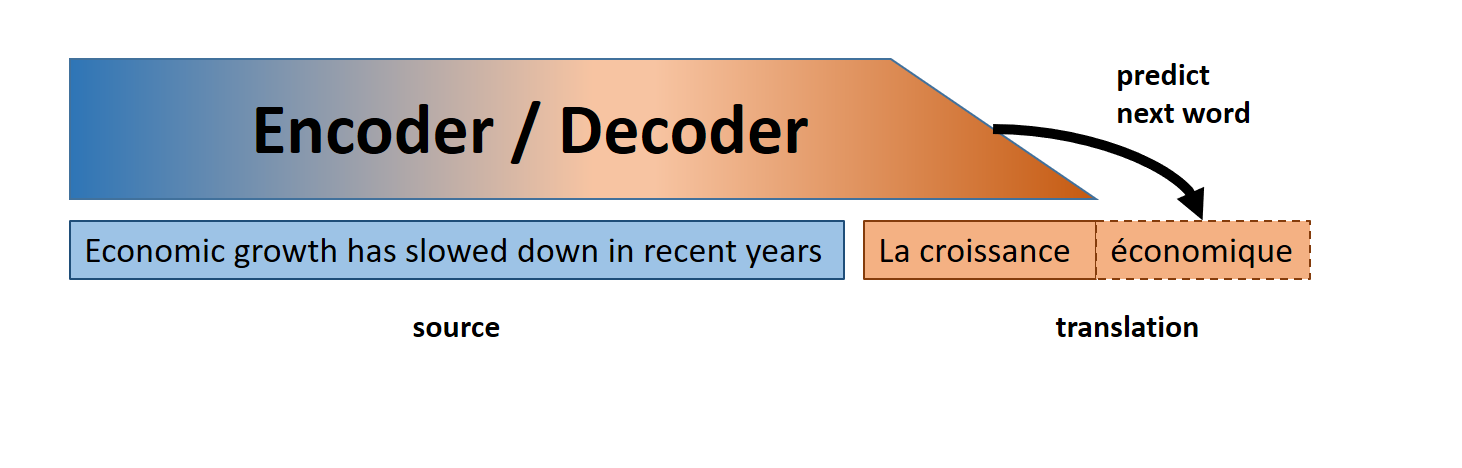
\includegraphics[width=12cm]{figure/arlm1.png}
	\end{figure}
	
\vfill

\end{frame}

% ------------------------------------------------------------------------------

\begin{frame}{Examples of ARLMs (1)}

\vfill

\textbf{Image Captioning:}

	\begin{figure}
		\centering
		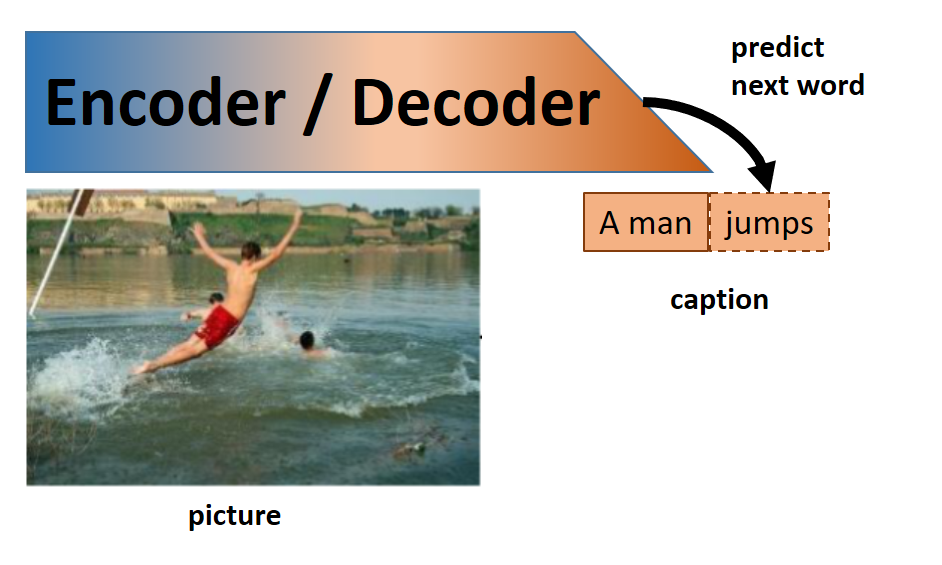
\includegraphics[width=8cm]{figure/arlm2.png}
	\end{figure}
\vfill

\end{frame}

% ------------------------------------------------------------------------------

\begin{frame}{Masked language models (MLM)}

\vfill

\begin{itemize}
	\item We have seen auto-regressive LMs
			\begin{itemize}
				\item context: previous words
				\item predict: next word
			\end{itemize}
	\item Another type: \textit{Masked} LMs (MLMs)
			\begin{itemize}
				\item context: surrounding words
				\item predict: masked word
			\end{itemize}
\end{itemize}

\vfill

\end{frame}

% ------------------------------------------------------------------------------

\begin{frame}{mlm: toy example}

\vfill

	\begin{figure}
		\centering
		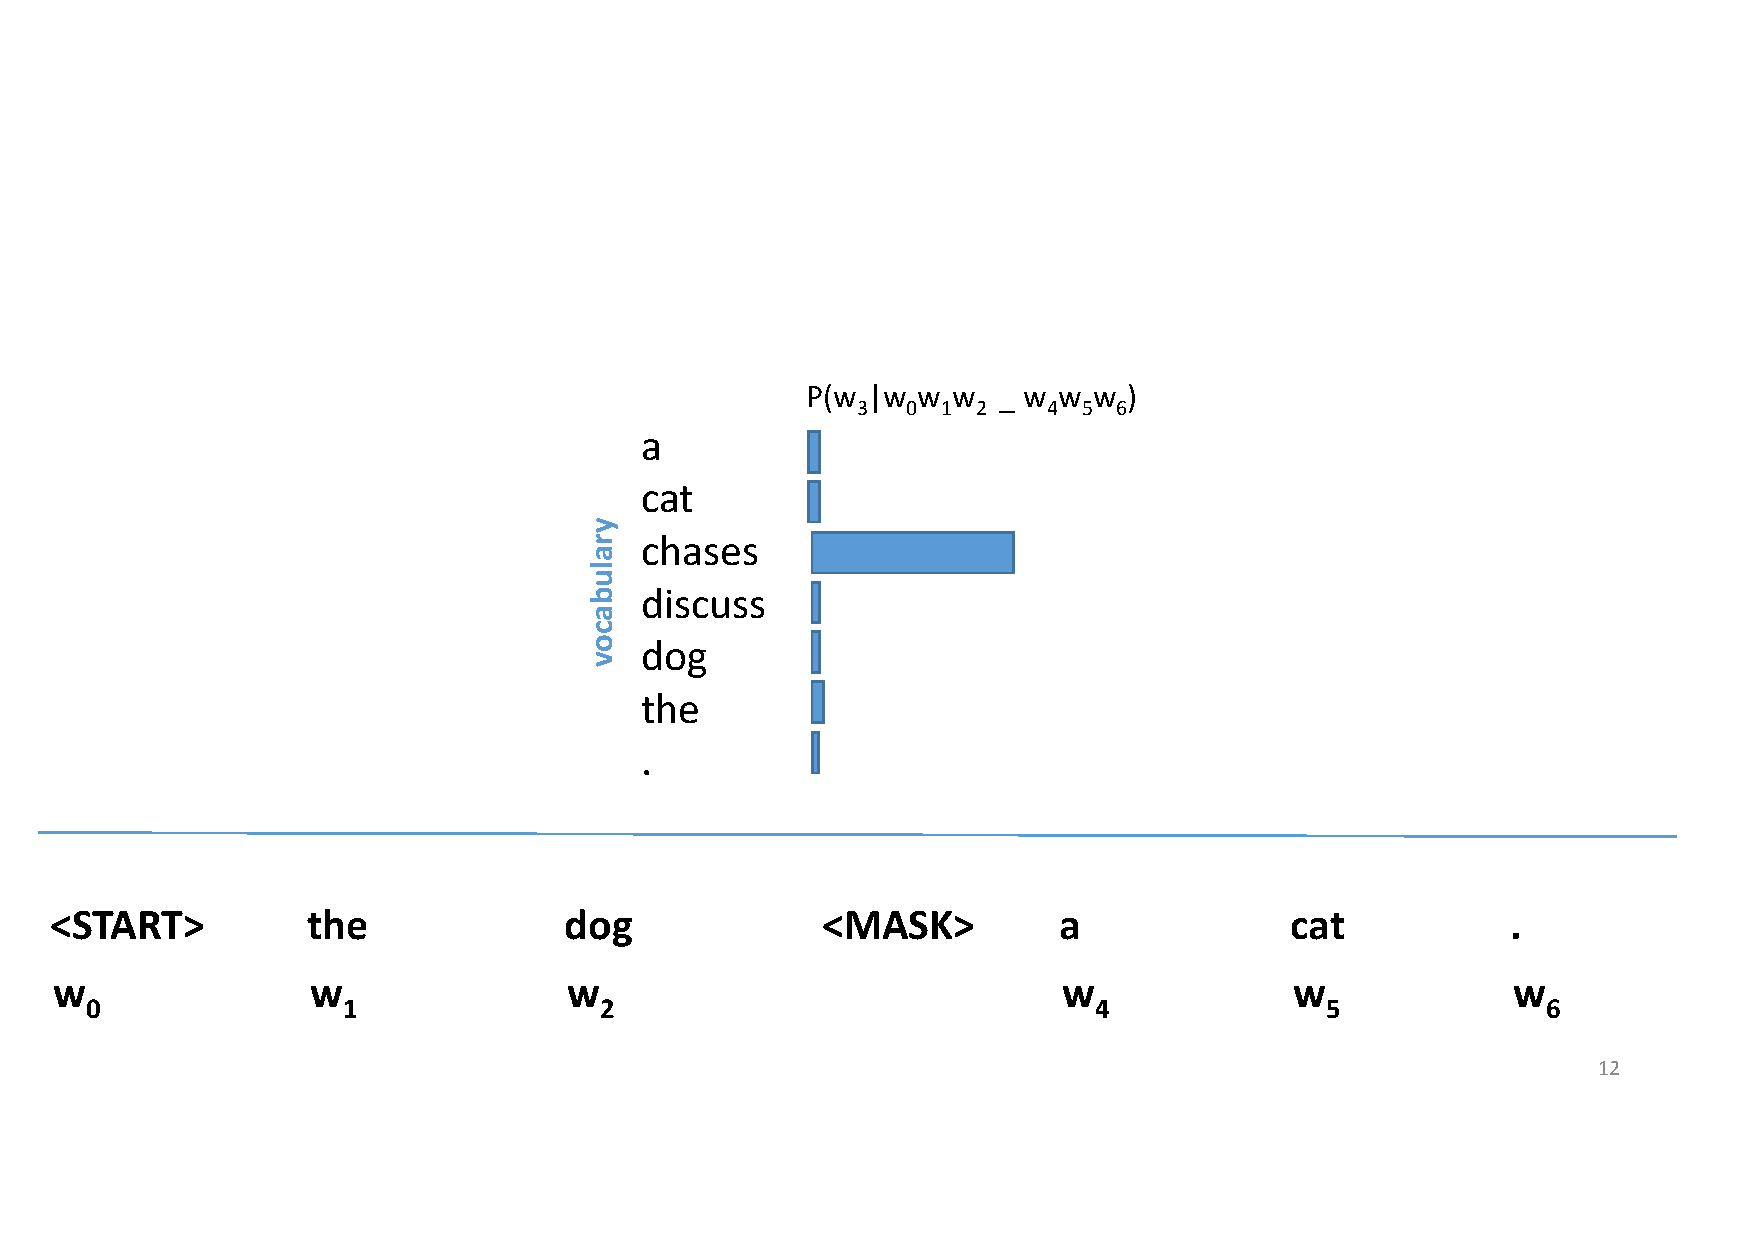
\includegraphics[width=8.50cm]{figure/mlm.pdf}
	\end{figure}
	
\vfill

\end{frame}

% ------------------------------------------------------------------------------

\begin{frame}{mlm: probabilistic interpretation}

\vfill

\begin{itemize}
	\item Estimates $P(w_i | w_0, w_1, w_{i-1}, \dots, w_{i+1}, w_n)$
	\item No ``clean`` estimate for $P(sentence)$, as
	$$ P(w_1, w_2, \dots, w_n | w_0)$$ $$\neq P(w_1 | w_0, w_2, \dots, w_n) \cdot P(w_2 | w_0, w_1, w_3, \dots, w_n)$$
	\item ARLMs are better than MLMs for generating texts 
	\item Advantage of MLMs: Learning contextualized representations
\end{itemize}

\vfill

\end{frame}

% ------------------------------------------------------------------------------


%%%%%%%%%%%%%%%%%%%%%%%%%%%%%%%%%%%%%%%%%%%%%%%%%%%%%%%%%%%%%%%%%%
\section{Measuring Performance}
% Source: DL4NLP chapter04-bert/slides-42-metrics.tex
%%%%%%%%%%%%%%%%%%%%%%%%%%%%%%%%%%%%%%%%%%%%%%%%%%%%%%%%%%%%%%%%%%
% ------------------------------------------------------------------------------

\begin{frame}{task-specific evaluation: classification}

\vfill

\textbf{(Binary) Document-level Classification}

\begin{itemize}
	\item Accuracy
	\item Recall / Precision
	\item F1-Score
	\item ROC-Curve / AUC
	\item ...
\end{itemize}

\textbf{(Multi-Class) Document-level classification}

\begin{itemize}
	\item Micro- / Macro-averaged F1
	\item Class-specific accuracies
	\item ...
\end{itemize}
\vfill

\end{frame}

% ------------------------------------------------------------------------------

\begin{frame}{task-specific evaluation: ranking (1)}

\vfill

\textbf{Ranking:}
%https://towardsdatascience.com/comprehensive-guide-to-ranking-evaluation-metrics-7d10382c1025

\begin{itemize}
		\item Use Cases:
				\begin{itemize}
					\item Retrieval systems output a ranking of relevant documents
					\item Search engines return top $k$ results
					\item ...
				\end{itemize}
		\item Ranking evaluation metrics
				\begin{itemize}
					\item Mean average precision (MAP)
					\item Mean reciprocal rank (MRR)
					\item Precision@k / Recall@k
					\item ...
				\end{itemize}
\end{itemize}
\vfill

\end{frame}

% ------------------------------------------------------------------------------

\begin{frame}{task-specific evaluation: ranking (2)}

\vfill

\textbf{MAP:}

\begin{figure}
    \centering
    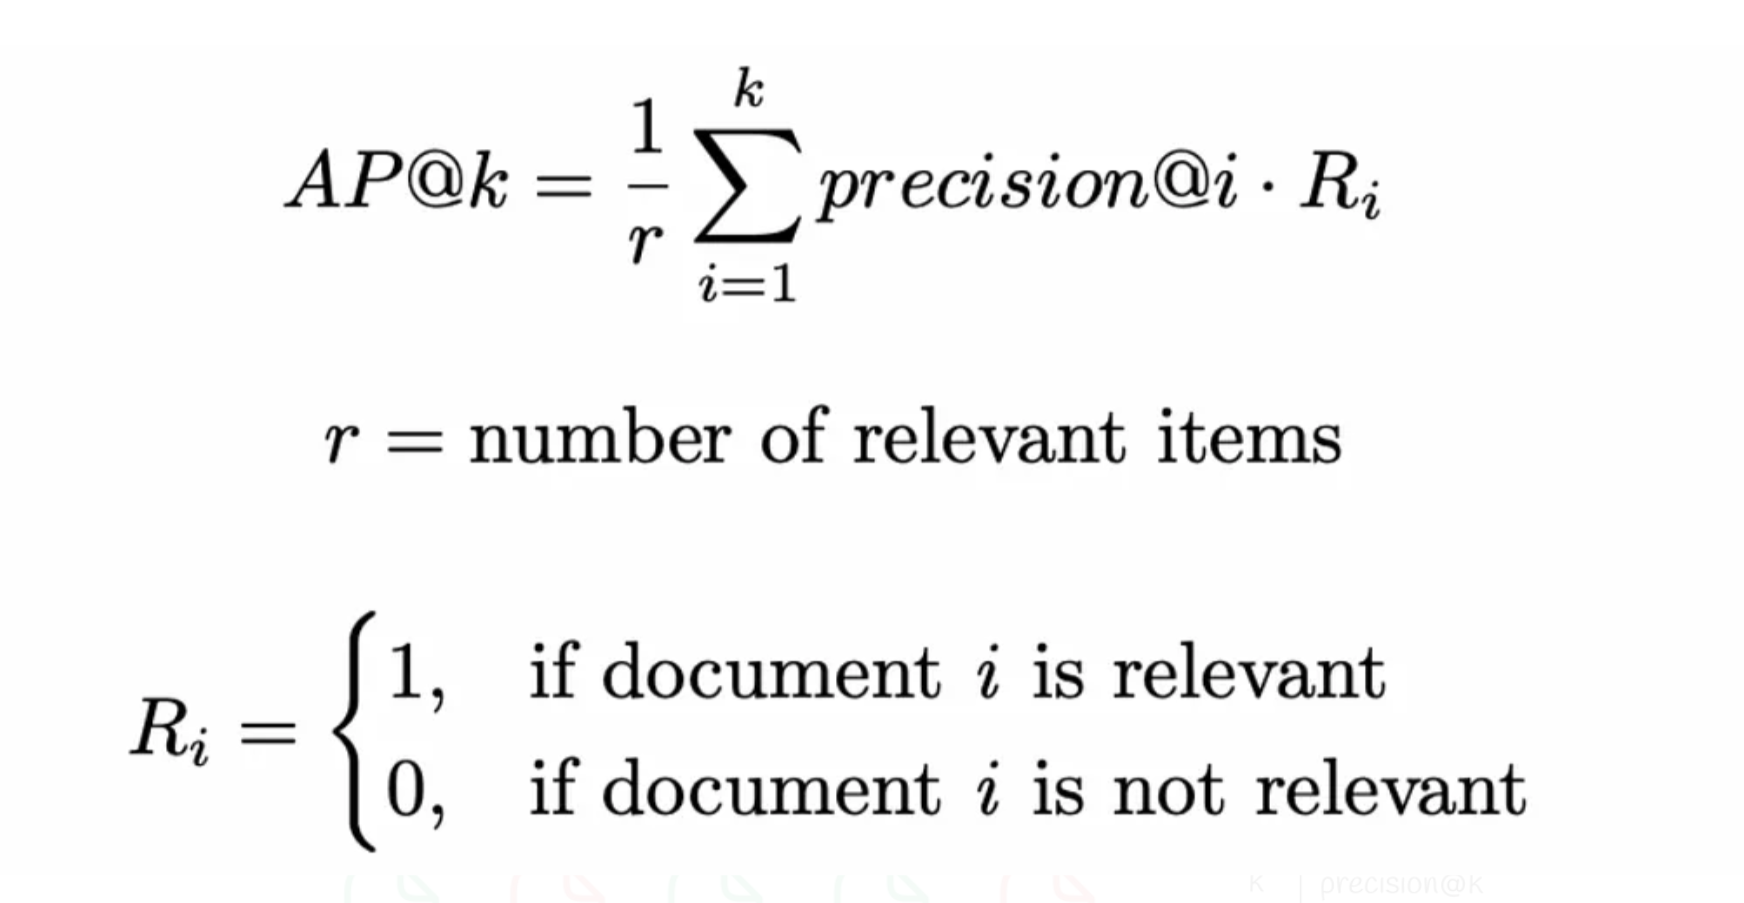
\includegraphics[width=9cm]{figure/42-ap.png}
		\citebutton{Source: towardsdatascience}{https://towardsdatascience.com/comprehensive-guide-to-ranking-evaluation-metrics-7d10382c1025}
\end{figure}

\vfill

\end{frame}

% ------------------------------------------------------------------------------

\begin{frame}{task-specific evaluation: ranking (3)}

\vfill

\textbf{Example MAP:}

\begin{figure}
    \centering
    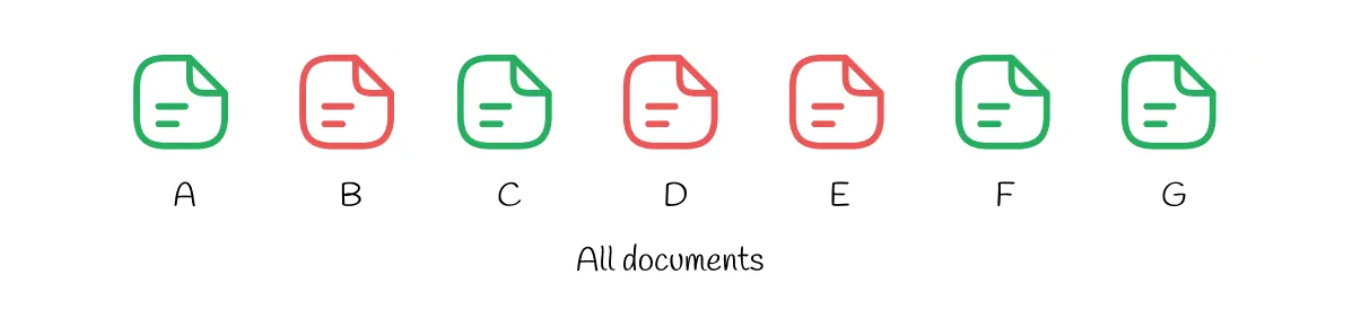
\includegraphics[width=9cm]{figure/42-ap-ex1.png}
		\citebutton{Source: towardsdatascience}{https://towardsdatascience.com/comprehensive-guide-to-ranking-evaluation-metrics-7d10382c1025}
\end{figure}

\vfill

\end{frame}

% ------------------------------------------------------------------------------

\begin{frame}{task-specific evaluation: ranking (4)}

\vfill

\textbf{Example MAP:}

\begin{figure}
    \centering
    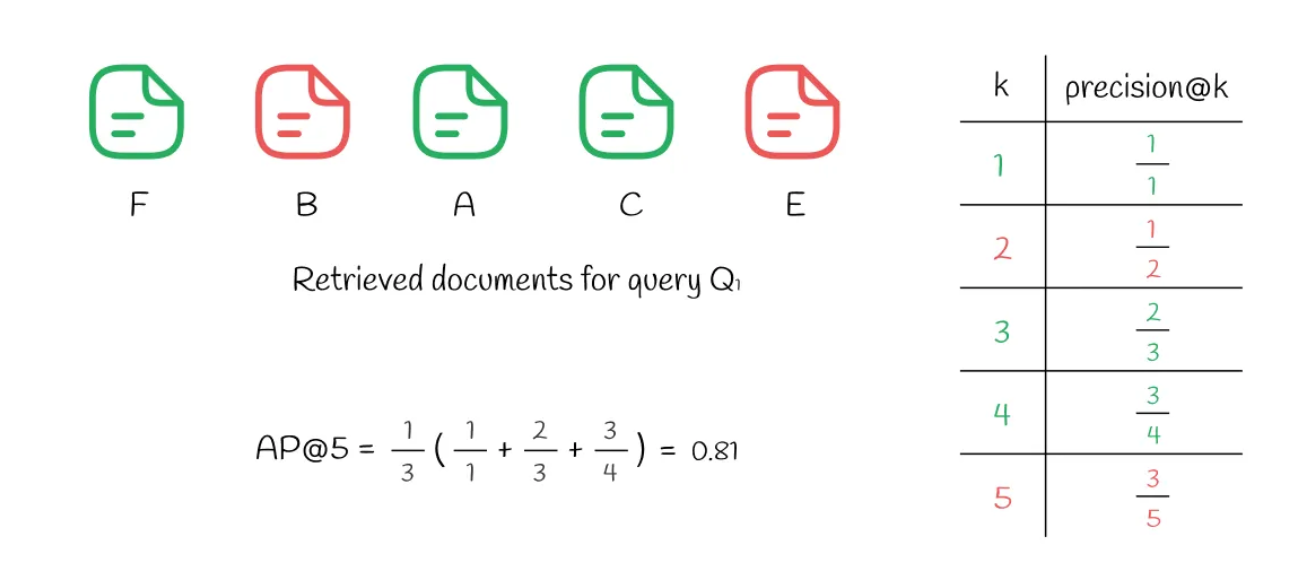
\includegraphics[width=9cm]{figure/42-ap-ex2.png}
		\citebutton{Source: towardsdatascience}{https://towardsdatascience.com/comprehensive-guide-to-ranking-evaluation-metrics-7d10382c1025}
\end{figure}

\vfill

\end{frame}

% ------------------------------------------------------------------------------

\begin{frame}{task-specific evaluation: ranking (5)}

\vfill

\textbf{Example MAP:}

\begin{figure}
    \centering
    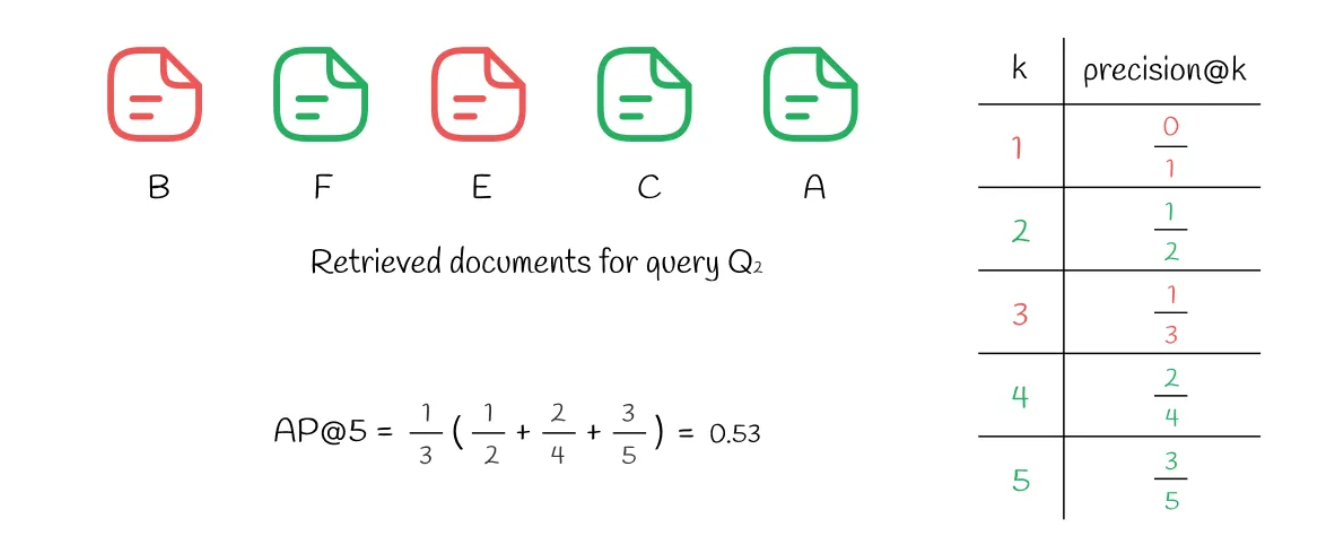
\includegraphics[width=9cm]{figure/42-ap-ex3.png}
		\citebutton{Source: towardsdatascience}{https://towardsdatascience.com/comprehensive-guide-to-ranking-evaluation-metrics-7d10382c1025}
\end{figure}

\vfill

\end{frame}

% ------------------------------------------------------------------------------

\begin{frame}{task-specific evaluation: ranking (6)}

\vfill

\textbf{MAP:}
%https://towardsdatascience.com/comprehensive-guide-to-ranking-evaluation-metrics-7d10382c1025

$$MAP = \dfrac{1}{|Q|} \sum_{q \in Q} Ap_q@k,\; with\; Q = \text{set of queries}$$

\begin{figure}
    \centering
    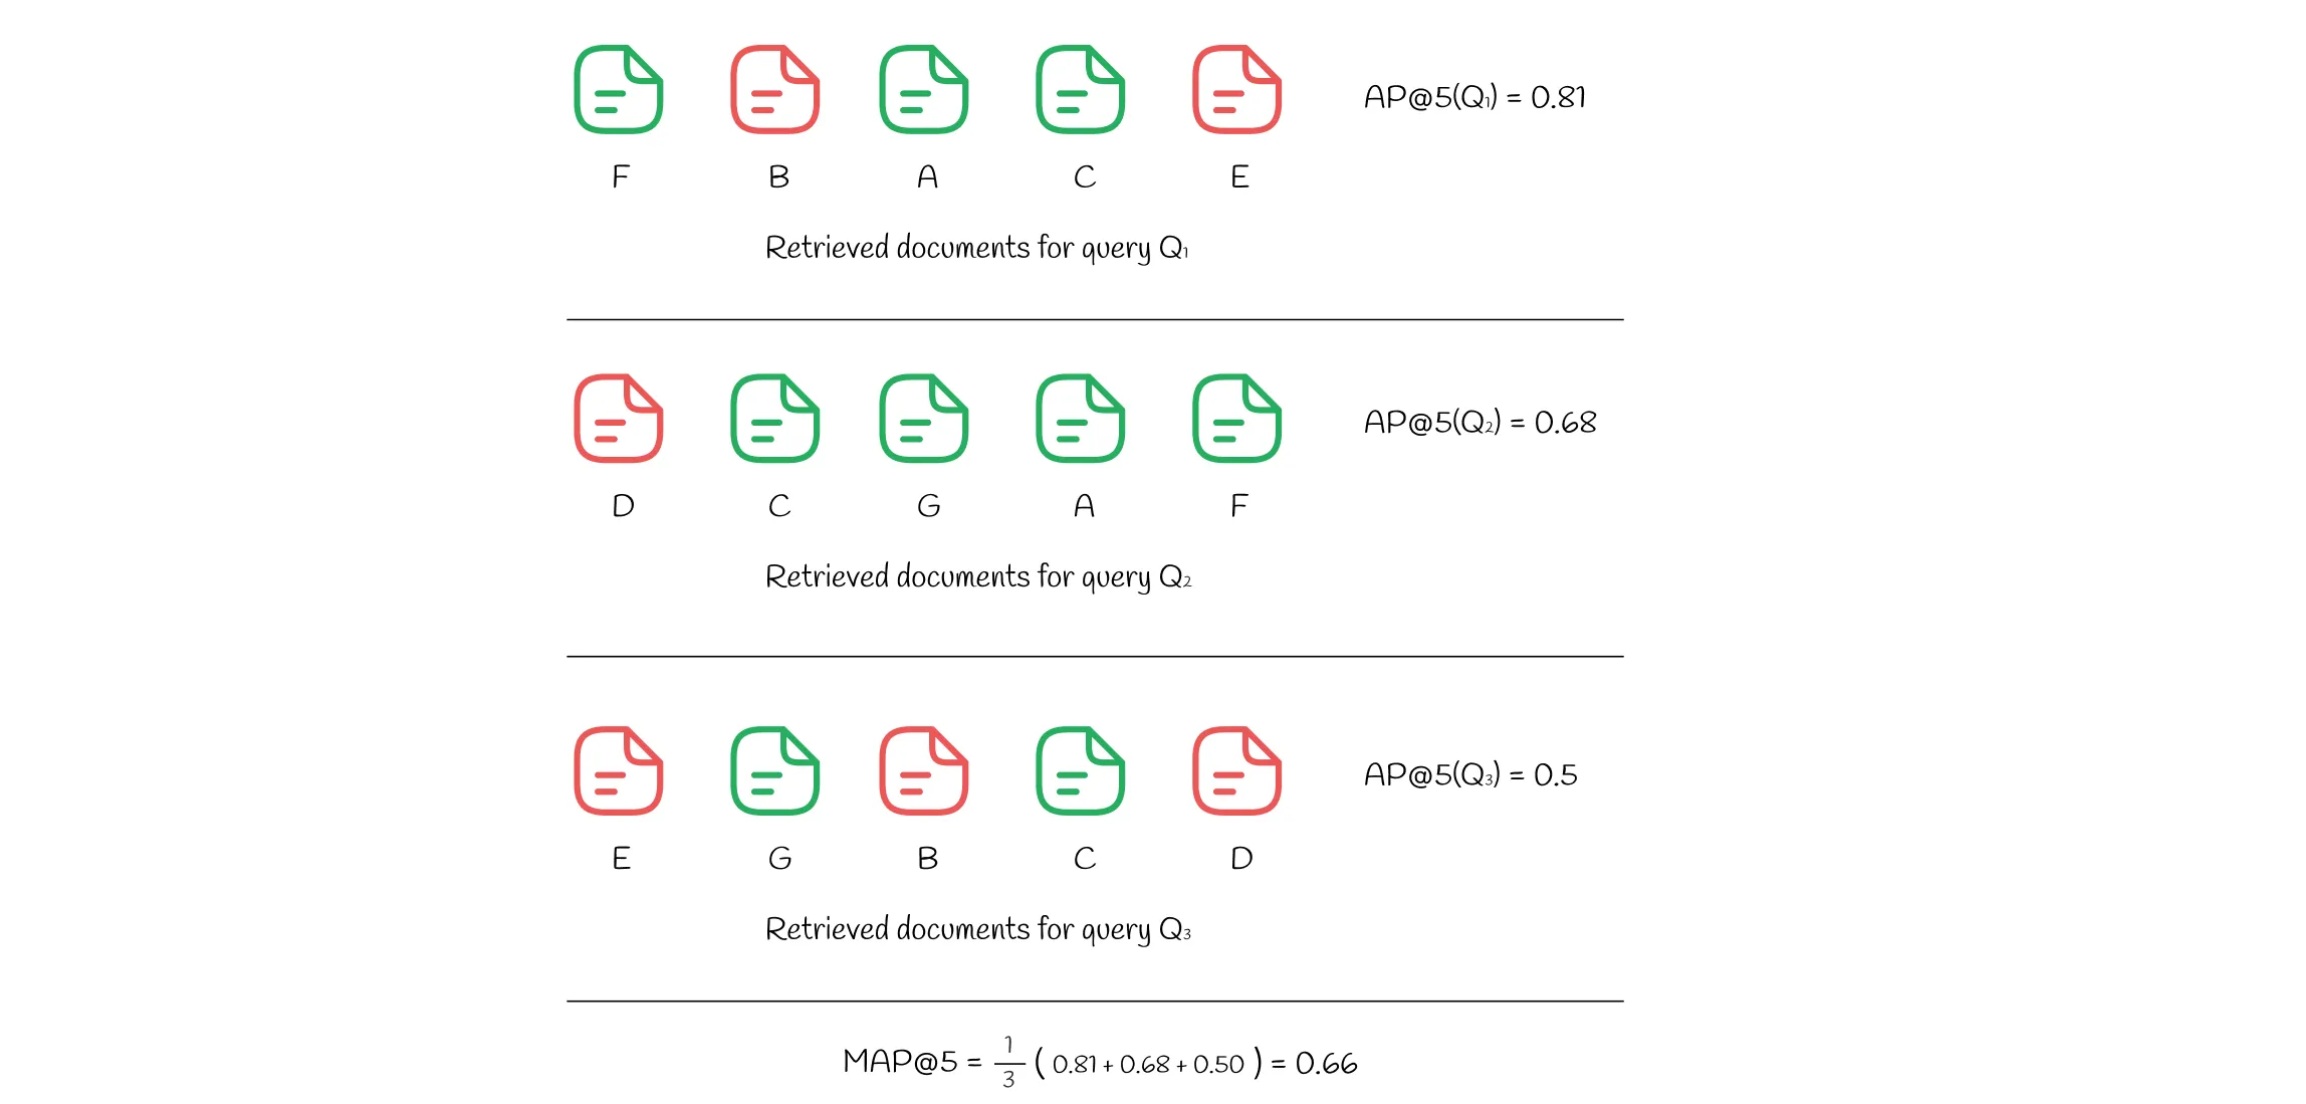
\includegraphics[width=7.65cm]{figure/42-ap-ex4.png}
		\citebutton{Source: towardsdatascience}{https://towardsdatascience.com/comprehensive-guide-to-ranking-evaluation-metrics-7d10382c1025}
\end{figure}

\vfill

\end{frame}

% ------------------------------------------------------------------------------

\begin{frame}{task-specific evaluation: ranking (7)}

\vfill

\textbf{MRR:}
%https://towardsdatascience.com/comprehensive-guide-to-ranking-evaluation-metrics-7d10382c1025

$$RR = \dfrac{1}{\text{rank of first relevant item}}$$
$$MRR = \dfrac{1}{|Q|} \sum_{q \in Q} RR_q,\; with\; Q = \text{set of queries}$$

\vfill

\end{frame}

% ------------------------------------------------------------------------------

\begin{frame}{ARLMs}

\vspace{-1cm}

	\begin{figure}
		\centering
		\includegraphics[width=10cm,page=13]{figure/arlm.pdf}
	\end{figure}
	
\begin{itemize}
	\item \ques How can we measure ``performance`` on this task? 
\end{itemize}

\vfill

\end{frame}

% ------------------------------------------------------------------------------

\begin{frame}{arlm perplexity (1)}

\vfill

\begin{itemize}
	\item Natural choice for evaluating generated text
	\item Well-defined for ARLMs; trickier for MLMs
	\item Intuitively: \textit{Amount of the model's surprisal when confronted with a sequence} (higher value means higher ``surprisal``)
	\item More technically: Measure of uncertainty of a probabilistic model
	\item Example: Perplexity of a fair $k$-sided die (uniform distribution) is $k$
\end{itemize}

\vfill

\end{frame}

% ------------------------------------------------------------------------------

\begin{frame}{arlm perplexity (2)}

\vfill
\begin{itemize}
	\item Autoregressive factorization of the sequence:
\end{itemize}

\begin{figure}
    \centering
    \animategraphics[loop,autoplay,height=1.5cm]{2}{figure/ppl_full/frame_}{0}{11}
		\citebutton{Source: huggingface}{https://huggingface.co/docs/transformers/perplexity}
\end{figure}

\begin{itemize}
	\item Log-probability of i-th token given context: $\log(p_\theta(w_i|w_{<i}))$
	\item[] more ``certain`` model $\to$ higher log-probability
	\item Aggregate$^1$ over the whole sequence:
				$$PPL = \exp\left(- \frac{1}{t} \sum_{i=1}^t \log(p_\theta(w_i|w_{<i}))\right)$$
\end{itemize}

\vfill

\footnotesize{$^1$The choice of the log’s base is basically arbitrary.}

\end{frame}

% ------------------------------------------------------------------------------

\begin{frame}{arlm perplexity (3)}

\vfill

\begin{itemize}
	\item \textit{Lower bound} is \textbf{1}, i.e. the model predicts \textit{every} token correctly (with a certainty of 100\%)
	\item \ques Is this really desirable?
	\item \textit{Upper bound} is $|V|$, i.e. the model only provides a random guess for every token with a probability of $\frac{1}{|V|}$
	\item Selection of state-of-the-art perplexities:
			\begin{itemize}
				\item \textbf{1B Word Benchmark} \citebutton{Chelba et al., 2013}{https://arxiv.org/abs/1312.3005} ($|V| = 800k$)\\
				PPL = 21,8 \citebutton{Dai et al., 2019}{https://aclanthology.org/P19-1285/}
				\item \textbf{WikiText-103} \citebutton{Merity et al., 2016}{https://arxiv.org/abs/1609.07843} ($|V|$ = 270k)\\
				PPL = 10,8 \citebutton{Shoeybi et al., 2019}{https://arxiv.org/abs/1909.08053}
				\item \textbf{Penn Treebank} \citebutton{Marcus et al., 1994}{https://aclanthology.org/H94-1020/} ($|V| = 10k$)\\
				PPL = 20,5 \citebutton{Brown et al., 2020}{https://proceedings.neurips.cc/paper_files/paper/2020/file/1457c0d6bfcb4967418bfb8ac142f64a-Paper.pdf}
			\end{itemize}
\end{itemize}

\vfill

\end{frame}

% ------------------------------------------------------------------------------

\begin{frame}{arlm perplexity (4)}

\vfill

\begin{itemize}
	\item \textit{Problem:} Fixed context size of models (e.g. 1024 for GPT-2) 
\end{itemize}

\begin{figure}
    \centering
    \animategraphics[loop,autoplay,height=1.5cm]{2}{figure/ppl_sliding/frame_}{18}{23}
		\citebutton{Source: huggingface}{https://huggingface.co/docs/transformers/perplexity}
\end{figure}

\begin{itemize}
	\item \textit{Possible solution:} Sliding window strategy
	\item Close approximation to ``true`` autoregressive decomposition
	\item \textit{Drawback:} Computationally expensive (individual forward pass for each token)
\end{itemize}

\vfill

\end{frame}

% ------------------------------------------------------------------------------

\begin{frame}{arlm perplexity (5)}

\vfill

\ques\\ Is a language model with lower perplexity always a ``better`` model?

\vspace{.5cm}

\textbf{Some (Dis)Advantages of perplexity:}

\begin{itemize}
	\item \textbf{Pro:} Straight-forward applicable
	\item \textbf{Pro:} Does not depend on ``external`` labels
	\item \textbf{Con:} Not clear what value can be considered ``good``
	\item \textbf{Con:} Corpus-/language-specific measure
\end{itemize}

\vfill

\end{frame}

% ------------------------------------------------------------------------------

\begin{frame}{evaluating generated text (1)}

\vfill

\begin{itemize}
	\item \ques How else can we evaluate the quality of generated text?
	\item[]
	\item \textit{Use cases:} 
			\begin{itemize}
				\item Machine translation
				\item Question answering (extractive or abstractive)
				\item Dialogue generation
				\item Text summarization
				\item Image Captioning
				\item Code generation
			\end{itemize}
\end{itemize}

\vfill

\end{frame}

% ------------------------------------------------------------------------------

\begin{frame}{evaluating generated text (2)}

\vfill

\textbf{Machine Translation}

\begin{itemize}
	\item Metrics based on N-gram-overlap
			\begin{itemize}
				\item BLEU (cf. Chap. 3.1) \citebutton{Papineni et al., 2002}{https://aclanthology.org/P02-1040/}
				\item ROUGE \citebutton{Lin, 2004}{https://aclanthology.org/W04-1013/}
				\item METEOR \citebutton{Banerjee and Lavie, 2005}{https://aclanthology.org/W05-0909/}
			\end{itemize}
	\item Metrics based pre-trained (neural) models
			\begin{itemize}
				\item BertScore \citebutton{Zhang et al., 2019}{https://arxiv.org/abs/1904.09675}
				\item BLEURT \citebutton{Sellam et al., 2020}{https://aclanthology.org/2020.acl-main.704/}
				\item COMET \citebutton{Rei et al., 2020}{https://aclanthology.org/2020.emnlp-main.213/}
			\end{itemize}
\end{itemize}

\vfill

\end{frame}

% ------------------------------------------------------------------------------

\begin{frame}{evaluating generated text (3)}

\vfill

\begin{itemize}
	\item BLEU, ROUGE, METEOR:
			\begin{itemize}
				\item "Bilingual evaluation understudy", originally for machine translation
				\item Measures overlap of words, and longer word sequences of different sizes
				\item BLEU: unreliable per-example, but correlates with human judgments on an aggregate level \citebutton{Reiter, 2018}{https://aclanthology.org/J18-3002/}
			\end{itemize}
\end{itemize}

\vfill

\end{frame}

% ------------------------------------------------------------------------------

\begin{frame}{evaluating generated text (3)}

\vfill

\begin{itemize}
	\item BERTScore
			\begin{itemize}
				\item Based on pre-trained BERT model
				\item Also able to consider contextual similarities
				\item Correlates better with human judgements
			\end{itemize}
	\item BLEURT
			\begin{itemize}
				\item Better per-example quality estimation by fine-tuning on examples with judgements
				\item But: potential bias if tested systems are very different than training examples
			\end{itemize}
\end{itemize}

\vfill

\end{frame}

% ------------------------------------------------------------------------------

\begin{frame}{evaluating generated text (4)}

\vfill

\textbf{Question Answering / Summarization / Dialogues}

\begin{itemize}
	\item Aspects to consider
			\begin{itemize}
				\item Factual correctness
				\item Fluency
				\item Stylistic aspects
				\item Engagement
				\item ...
			\end{itemize}
	\item Human evaluation?! (cf. next slide)
\end{itemize}

\vfill

\end{frame}

% ------------------------------------------------------------------------------

\begin{frame}{human evaluation}

\vfill

\textbf{Pros}

\begin{itemize}
	\item Possible where simply using metrics fails (esp. generated texts)
	\item Probably gold standard (given trained human evaluator)
	\item \textit{Strong} learning signal for models (cf. RLHF, chapter 9)
	\item ...
\end{itemize}

\vspace{.3cm}

\textbf{Cons}

\begin{itemize}
	\item Manual, tedious work
  \item Costs and working conditions
	\item Subjectivity
	\item Ambiguity
	\item ...
\end{itemize}

\vfill

\end{frame}

% ------------------------------------------------------------------------------


%%%%%%%%%%%%%%%%%%%%%%%%%%%%%%%%%%%%%%%%%%%%%%%%%%%%%%%%%%%%%%%%%%
\section{The Architecture}
% Source: DL4NLP chapter04-bert/slides-43-corefacts.tex
%%%%%%%%%%%%%%%%%%%%%%%%%%%%%%%%%%%%%%%%%%%%%%%%%%%%%%%%%%%%%%%%%%
% ------------------------------------------------------------------------------

\begin{frame}{Predecessors of BERT}
\hbox{\hspace{-3em} 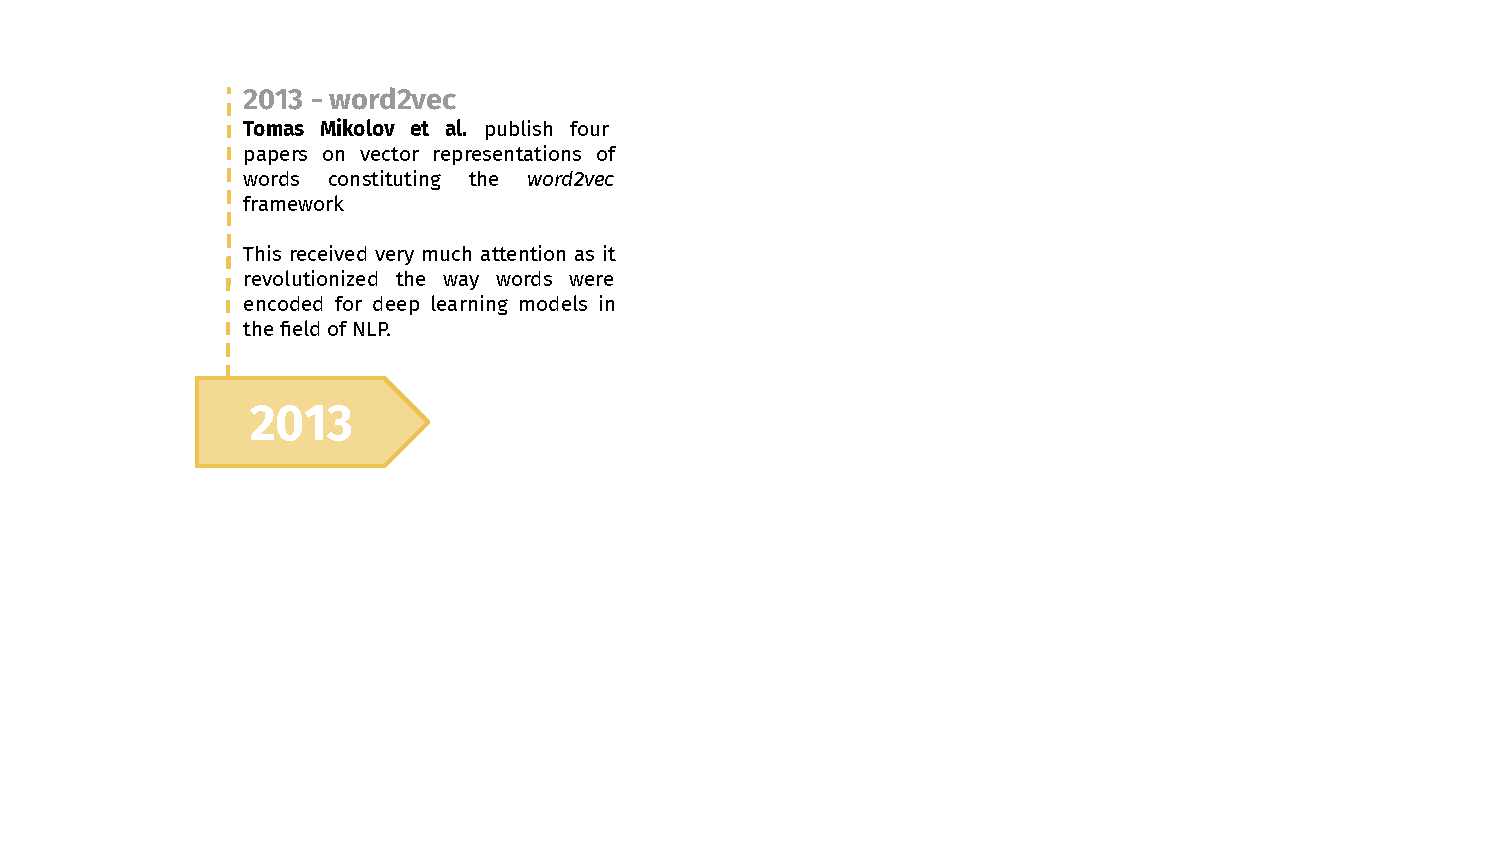
\includegraphics[width=12cm,page=1]{figure/transfer_learning_timeline1_nlp.pdf}}
\end{frame}
\begin{frame}[noframenumbering]{Predecessors of BERT}
\hbox{\hspace{-3em} \includegraphics[width=12cm,page=2]{figure/transfer_learning_timeline1_nlp.pdf}}
\end{frame}
\begin{frame}[noframenumbering]{Predecessors of BERT}
\hbox{\hspace{-3em} \includegraphics[width=12cm,page=3]{figure/transfer_learning_timeline1_nlp.pdf}}
\end{frame}
\begin{frame}[noframenumbering]{Predecessors of BERT}
\hbox{\hspace{-3em} \includegraphics[width=12cm,page=4]{figure/transfer_learning_timeline1_nlp.pdf}}
\end{frame}
\begin{frame}[noframenumbering]{Predecessors of BERT}
\hbox{\hspace{-3em} \includegraphics[width=12cm,page=5]{figure/transfer_learning_timeline1_nlp.pdf}}
\end{frame}

% ------------------------------------------------------------------------------

\begin{frame}{context: ulmfit and gpt}

\vfill

	\textbf{Shortcomings of ELMo:}

	\begin{itemize}
		\item No adaption of the Embeddings to target domain/task
		\item Sequential nature of LSTMs: Not fully parallelizable 
	\end{itemize}
	
	\textbf{Alleviations/Alternatives:}

	\begin{itemize}
		\item ULMFiT \citebutton{Howard and Ruder, 2018}{https://www.aclweb.org/anthology/P18-1031} is a uni-directional LSTM which is fine-tuned as a whole model on data from the target domain/task.
		\item GPT \citebutton{Radford et al., 2018}{https://s3-us-west-2.amazonaws.com/openai-assets/research-covers/language-unsupervised/language_understanding_paper.pdf} is a Transformer decoder which is fine-tuned as a whole model on data from the target domain/task.
	\end{itemize}
	
	\textbf{All three still not sufficient:}

	\begin{itemize}
		\item \textit{Bidirectionally contextual:} Only ELMo 
		\item \textit{Parallelizable:} Only GPT
		\item \textit{Fine-tune whole model:} Only ULMFiT \& GPT
	\end{itemize}
	
\vfill


\end{frame}

% ------------------------------------------------------------------------------

\begin{frame}{bert: key facts}

\vfill

\textit{\textbf{B}idirectional \textbf{E}ncoder \textbf{R}epresentations from \textbf{T}ransformers:}

\vspace{.5cm}

\begin{itemize}
		\item Bidirectionally contextual model\\
					$\to$ The embeddings of a single token depend on its left- and on its right-side context (similar to ELMo, but better)
		\item Completely replaces recurrent architectures by Self-Attention\\
					$\to$ parallelizable
		\item Model can be fine-tuned as a whole
\end{itemize}

\vfill

\end{frame}

% ------------------------------------------------------------------------------

\begin{frame}{ELMo vs. GPT vs. BERT}

\vfill

\begin{figure}
\centering
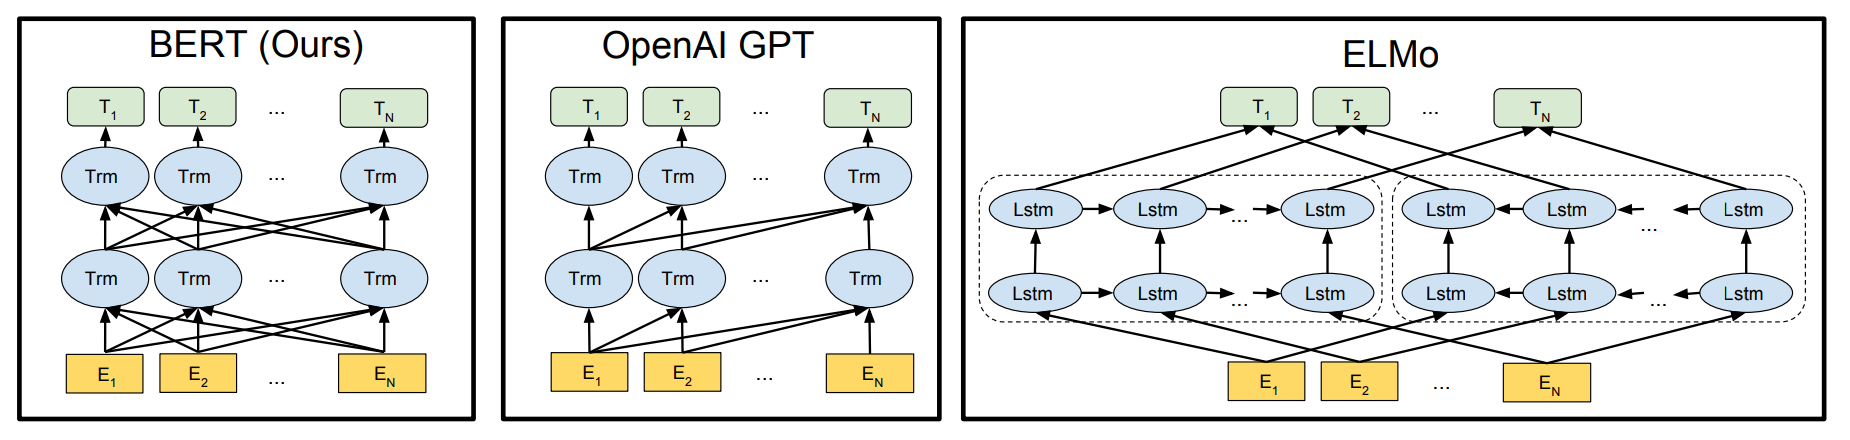
\includegraphics[width = 11cm]{figure/comparison-bert.png}\\ 
\citebutton{Source: Devlin et al., 2019}{https://aclanthology.org/N19-1423.pdf}
\end{figure}

\textbf{Major architectural differences:}

\begin{itemize}
\item ELMo uses two separate unidirectional models to achieve bidirectionality 
  $\rightarrow$ Only "\textit{shallow}" bidirectionality
\item GPT is not bidirectional, thus no issues concerning causality
\item BERT combines the best of both worlds: $$Self\text{-}Attention + (Deep)\;Bidirectionality$$
\end{itemize} 

\vfill

\end{frame}

% ------------------------------------------------------------------------------

\begin{frame}{bert: key facts}

\vfill

	\begin{itemize}
		\item New self-supervised objective(s)
		\item[] $\to$ MLM as \textit{necessity} for the architecture to work
		\item[] $\to$ Next-Sentence-Prediction as complementary objective\\(cf. next section)
		\item Transformer \textit{encoder} as backbone of the architecture
		\item 110M (340M) parameters in total for $BERT_{Base}$ ($BERT_{Large}$)
			\begin{itemize}
				\item 12 (24) Transformer encoder blocks
				\item Embedding size of $E = 768$ (1024)
				\item Hidden layer size $H = E$
				\item $A = H/64 = 12$ (16) attention heads
				\item Feed-forward size is set to $4H$
			\end{itemize}
	\end{itemize}

\vfill

\end{frame}

% ------------------------------------------------------------------------------

\begin{frame}{Core of BERT -- Transformer Encoder}

\begin{figure}
	\centering
		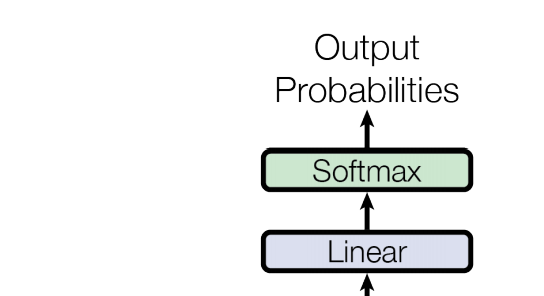
\includegraphics[width = 2.55cm]{figure/bert-top.png}\\ 
		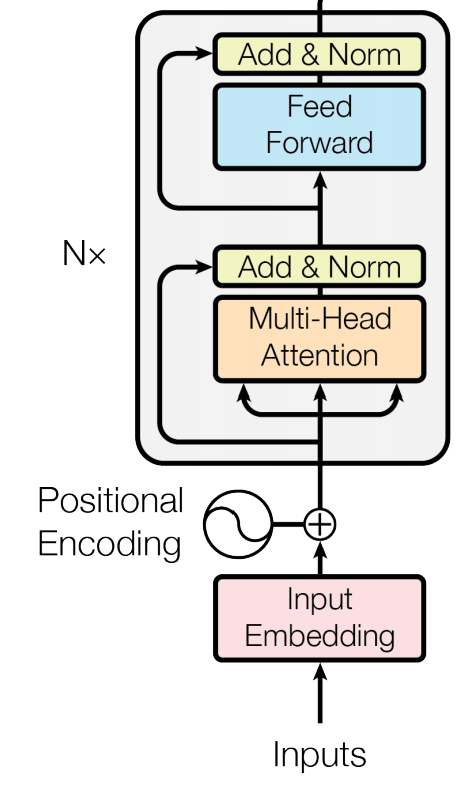
\includegraphics[width = 2.38cm]{figure/bert-bottom.png}\\ 
	\citebutton{Vaswani et al. (2017)}{https://arxiv.org/pdf/1706.03762.pdf}
\end{figure}

\end{frame}

% ------------------------------------------------------------------------------

\begin{frame}{A remark on "Causality"}

\vfill

\textbf{Causality is an issue!}
	
\begin{itemize}
	\item Goal: Learn contextual representations for words/tokens
	\item \textit{Self-Supervision:} Input and target sequence are the same\\
				$\rightarrow$ We modify the input to create a meaningful task 
	\item \warning Unconstrained Self-Attention makes using the LM objective infeasible
	\item \ques Why is this the case?
	\pause
	\item[] Bidirectionality at a lower layer would allow a word to see itself at later hidden layers\\
				$\rightarrow$ The model would be allowed to cheat!\\
				$\rightarrow$ This would not lead to meaningful internal representations
\end{itemize}

\vfill

\end{frame}

% ------------------------------------------------------------------------------

\begin{frame}{bert -- input embeddings}

\vfill

\begin{figure}
	\centering
	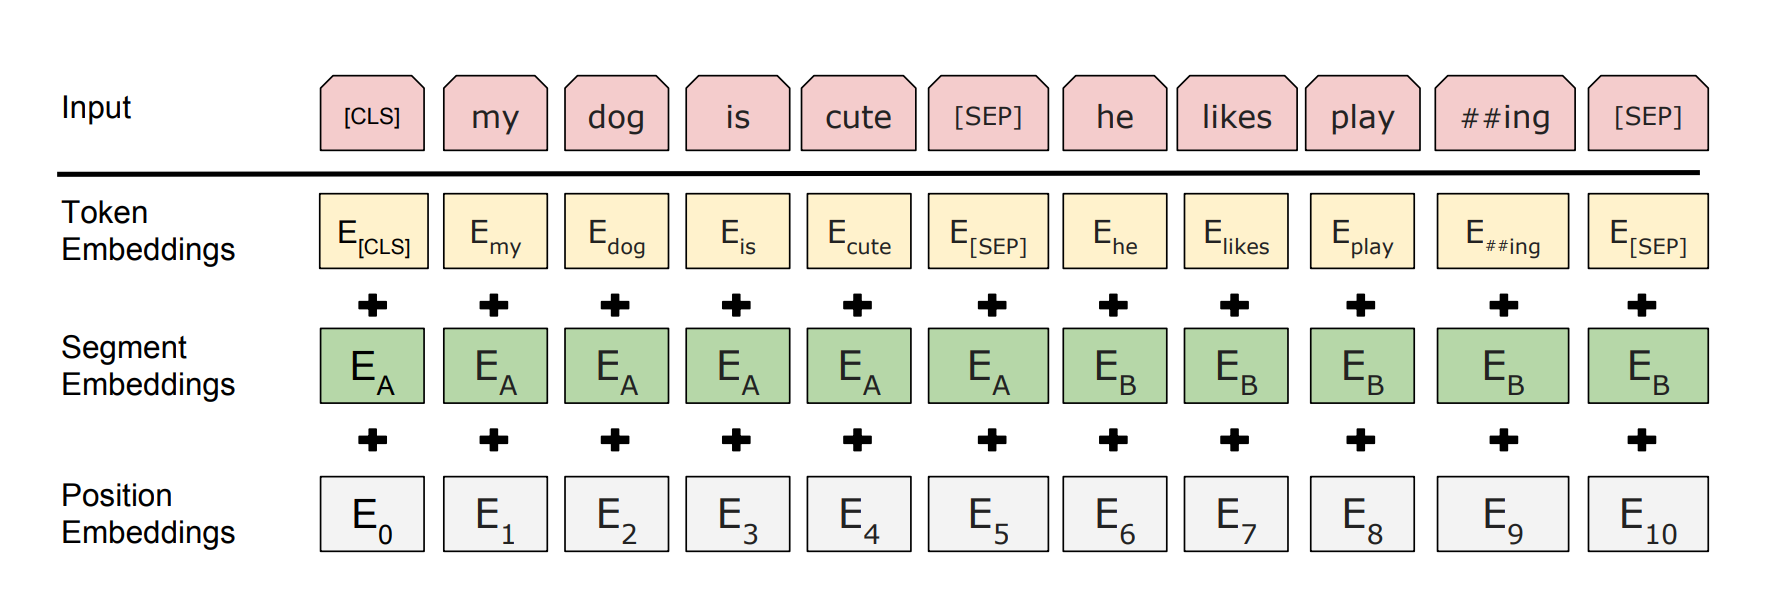
\includegraphics[width = 10cm]{figure/bert-input.png}\\ 
	\citebutton{Source: Devlin et al., 2019}{https://aclanthology.org/N19-1423.pdf}
\end{figure}

\begin{itemize}
	\item Two concatenated sentences as input
	\item WordPiece tokenization \citebutton{Wu et al., 2016}{https://arxiv.org/abs/1609.08144} for the inputs\\
			$\rightarrow$ Vocabulary of 30.000 tokens
	\item \textit{Learned} segment $+$ position embeddings
	\item Special \texttt{[CLS]} and \texttt{[SEP]} tokens
\end{itemize}

\vfill

\end{frame}

% ------------------------------------------------------------------------------

\begin{frame}{bert -- all embeddings}

\vfill

\begin{figure}
	\centering
	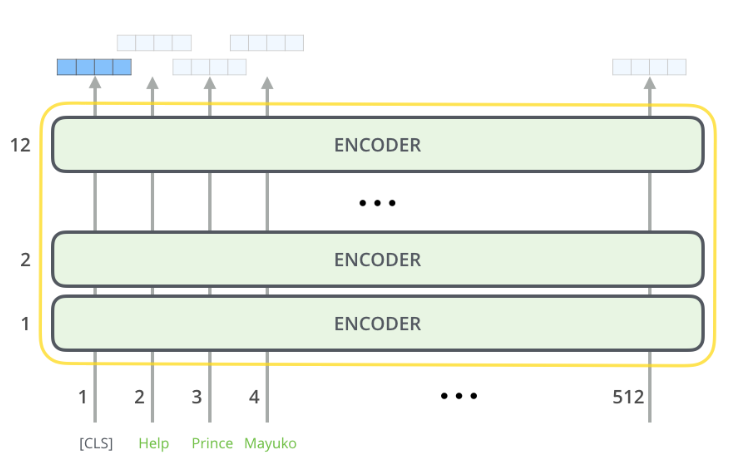
\includegraphics[width = 6.80cm]{figure/bert-embedings.png}\\ 
		\citebutton{Source: Jay Alammar}{https://jalammar.github.io/illustrated-bert/}
\end{figure}

\begin{itemize}
	\item One embedding per token per layer
	\item Non-contextual embeddings in the very first embedding layer
	\item More contextualization deeper into the model
\end{itemize}

\vfill

\end{frame}

% ------------------------------------------------------------------------------

\begin{frame}{bert -- the role of [CLS] and [SEP]}

\vfill

\textbf{Why deliberately include extra ``words``?}

\begin{itemize}
	\item The \texttt{[CLS]} token serves as an overall embedding for representing the whole sequence\\
				$\to$ Later on (cf. next chapter) BERT can thus used for classifying whole sequences\\
				$\to$ Can be extracted and used for clustering or similar
	\item The \texttt{[SEP]} (short for ```separator`) token serves as a ``signal`` for the model when used for taks on pairs of sequences
\end{itemize}

\textbf{Note:}

\begin{itemize}
	\item One further ``special`` token: \texttt{[UNK]} for representing unknown tokens or symbols (so the don't ``break`` the model)
\end{itemize}

\vfill

\end{frame}

% ------------------------------------------------------------------------------

\begin{frame}{Two different BERT versions}
\textit{There are two different BERT versions, namely BERT base and large. Depending on the architecture we get different parameter counts} \citebutton{Source: Devlin et al., 2019}{https://arxiv.org/abs/1810.04805}

\begin{itemize}
	\item \textbf{BERT base:}
	\begin{itemize}
		\item $n_{layers} = 12$, we have 12 encoder layers
		\item $n_{heads} = 12$, this will not affect the parameter count since they perfectly split $d_{model}$ across the heads
		\item $d_{model} = 768$, thats the embedding dimension
	\end{itemize}

	\item \textbf{BERT large:}
	\begin{itemize}
		\item $n_{layers} = 24$
		\item $n_{heads} = 16$
		\item $d_{model} = 1024$
	\end{itemize}
\end{itemize}
	
\end{frame}

%-------------------------------------------------------------------------------

\begin{frame}{Encoder Parameter Count}

\textit{From the chapter about the transformer parameter count we already know the number of parameters for one Encoder layer: $12\cdot d_{model}^2$}
$$
N_{Encoder} = n_{layers} \cdot 12\cdot d_{model}^2
$$

\begin{itemize}
	\item \textbf{BERT base}:
	$$N_{Encoder} = 12\cdot 12\cdot 768^2 = 84,934,656$$
	\item \textbf{BERT large}:
	$$N_{Encoder} = 24\cdot 12\cdot 1024^2 = 301,989,888$$
\end{itemize}

\textit{By increasing $d_{model}$ and $n_{layers}$ we more than tripled the number of Encoder parameters!}
\end{frame}

%-------------------------------------------------------------------------------

\begin{frame}{Embedding Parameter Count}
\textit{Similar to the Transformer chapter we also have to consider the paramters from the embeddings:}

\begin{itemize}
	\item Let $V$ be the vocabulary size, $M$ the maximum sequence length and $S$ the number of segments
	\item BERT has three kinds of embeddings, which are all learned:
	\begin{itemize}
		\item $V \times d_{model}$ token embeddings
		\item $S \times d_{model}$ segment embeddings
		\item $M \times d_{model}$ position embeddings
	\end{itemize}
	\item From the BERT paper we know $V=30000$, $S = 2$ and $M = 512$ 
	\item \textbf{BERT base}:
	$$N_{Embedding} = 30000\times 768 + 2\times 768 + 512\times 768 = 23,434,752$$
	\item \textbf{BERT large}:
	$$N_{Embedding} = 30000\times 1024 +2\times 1024 + 512\times 1024 = 31,246,336$$
\end{itemize}
	
\end{frame}

%-------------------------------------------------------------------------------

\begin{frame}{Final Parameter Count}

\bigskip

\textit{Now we just have to sum up both parts to get the final parameter count:}

\bigskip

\begin{itemize}
	\item \textbf{BERT base}: 
	$$N_{Total} = 84,934,656 + 23,434,752 = 108,369,408 \approx 110M$$
	\item[]
	\item \textbf{BERT large}:
	$$N_{Total} = 301,989,888 + 31,246,336 = 333,236,224 \approx 340M$$
\end{itemize}
	
\end{frame}

% ------------------------------------------------------------------------------


%%%%%%%%%%%%%%%%%%%%%%%%%%%%%%%%%%%%%%%%%%%%%%%%%%%%%%%%%%%%%%%%%%
\section{Pre-training \& Fine-Tuning}
% Source: DL4NLP chapter04-bert/slides-44-pretrain-finetune.tex
%%%%%%%%%%%%%%%%%%%%%%%%%%%%%%%%%%%%%%%%%%%%%%%%%%%%%%%%%%%%%%%%%%
% ------------------------------------------------------------------------------

\begin{frame}{Masked Language Modeling (MLM)}

\vfill

\textbf{First remark:}

\begin{itemize}
	\item Distinguish from \textit{Masked Self-Attention}\\ 
				$\to$ Masked Self-Attention is an architectural detail in the decoder of the Transformer, i.e. used by e.g. GPT
	\item Masked Self-Attention as a way to prevent causality issues in a Transformer decoder 
	\item MLM is a self-supervised \textit{modeling objective} introduced to couple Self-Attention and (deep) bidirectionality without violating causality
\end{itemize}

\vfill

\end{frame}

% ------------------------------------------------------------------------------

\begin{frame}{MLM (2)}

\begin{itemize}
\item \textbf{Training objective:} $$\text{Given a sentence, predict \texttt{[MASK]}ed tokens}$$
\item \textbf{Generation of samples:} $$\text{Randomly replace* a fraction of the words by \texttt{[MASK]}}$$
  \scriptsize *Sample 15\% of the tokens; replace 80\% of them by \texttt{[MASK]}, 10\% by a random token \& leave 10\% unchanged
\item \normalsize \textbf{Input:}\\\mbox{}\\
			\footnotesize
\begin{tabular}{|cccccccccc|}
\hline
The & quick & brown & \cellcolor{blue!65}\texttt{[MASK]} & jumps & over & the & \cellcolor{blue!65}\texttt{[MASK]} & dog & . \\
\hline
\end{tabular}\\\mbox{}
\item \normalsize \textbf{Targets:} $$(fox,\; lazy)$$
\end{itemize}

\end{frame}

% ------------------------------------------------------------------------------

\begin{frame}{MLM (3)}

\begin{itemize}
\item \warning But 20\% of the samples will look different!\\
			$\to$ 10\% replaced by a random token; 10\% left unchanged
\item \normalsize \textbf{Input (first case):}\\\mbox{}\\
			\footnotesize
\begin{tabular}{|cccccccccc|}
\hline
The & quick & brown & \cellcolor{blue!65}\texttt{orange} & jumps & over & the & \cellcolor{blue!65}\texttt{is} & dog & . \\
\hline
\end{tabular}\\\mbox{}
\item \normalsize \textbf{Targets (first case):} $$(fox,\; lazy)$$
\item \normalsize \textbf{Input (second case):}\\\mbox{}\\
			\footnotesize
\begin{tabular}{|cccccccccc|}
\hline
The & quick & brown & \cellcolor{blue!65}\texttt{fox} & jumps & over & the & \cellcolor{blue!65}\texttt{lazy} & dog & . \\
\hline
\end{tabular}\\\mbox{}
\item \normalsize \textbf{Targets (second case):} $$(fox,\; lazy)$$
\end{itemize}

\end{frame}
% ------------------------------------------------------------------------------

\begin{frame}{MLM (4)}

\vfill

\textbf{Discrepancy between pre-training \& fine-tuning:}

\begin{itemize}
	\item \texttt{[MASK]}-token as central part of pre-training procedure
	\item \texttt{[MASK]}-token does not occur during fine-tuning
	\item \textbf{Modified pre-training task:}\\
				Predict 15\% of the tokens of which only 80\% have been replaced by \texttt{[MASK]}
				\begin{itemize}
					\item 80\% of the selected tokens are actually \texttt{[MASK]}ed
					\item 10\% of the selected tokens: The model has to ``understand`` that the word needs to be \textit{replaced}
					\item 10\% of the selected tokens: The model has to ``understand`` that the word needs to be \textit{kept}
			\end{itemize}
	\item This ensures overlap between the kind data seen during pre-training and during fine-tuning
\end{itemize}
	
\vfill

\end{frame}

% ------------------------------------------------------------------------------

\begin{frame}{MLM (5)}

\vfill

	\begin{figure}
		\centering
		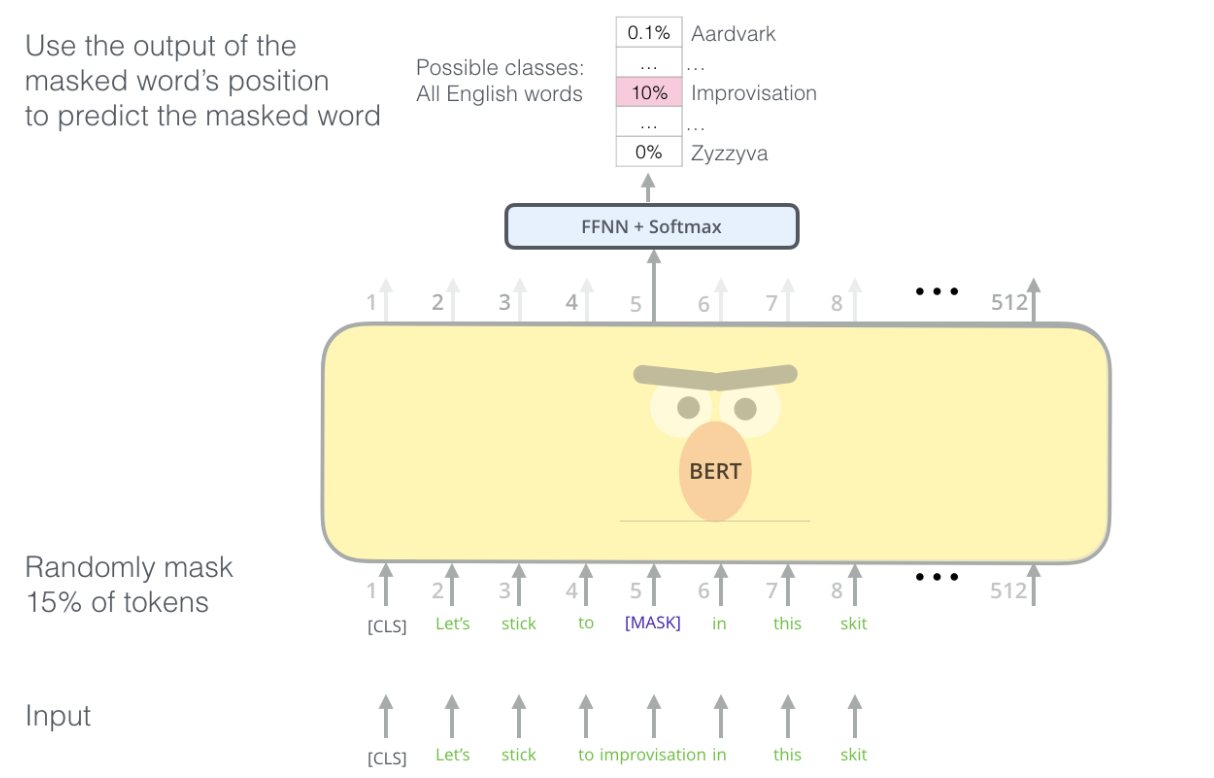
\includegraphics[width = 8.50cm]{figure/bert-mlm.png}\\ 
		\citebutton{Source: Jay Alammar}{https://jalammar.github.io/illustrated-bert/}
	\end{figure}

\vfill

\end{frame}

% ------------------------------------------------------------------------------

\begin{frame}{Next Sentence Prediction (NSP)}

\begin{itemize}
\item \textbf{Training objective:} $$\text{Given two sentences, predict whether $s_2$ follows $s_1$}$$
\item \textbf{Generation of samples:} $$\text{Randomly sample* negative examples (cf. word2vec)}$$
  \scriptsize *50\% of the time the second sentence is the actual next sentence, 50\% of the time it is a randomly sampled sentence
\item \normalsize \textbf{Full Input:}\\\mbox{}\\
			\footnotesize
\begin{center}
\begin{tabular}{|cccccccc|}
\hline
\cellcolor{blue!15}\texttt{[CLS]} & The & \cellcolor{blue!65}\texttt{[MASK]} & is & quick & . & \cellcolor{blue!15}\texttt{[SEP]} &\\\hline\hline It & jumps & over & the & \cellcolor{blue!65}\texttt{[MASK]} & dog & . & \cellcolor{blue!15}\texttt{[SEP]} \\
\hline
\end{tabular}\\\mbox{}
\end{center}
\item \normalsize \texttt{[CLS]} token as sequence representation for classification
\item \texttt{[SEP]} token for separation of the two input sequences
\end{itemize}

\end{frame}

% ------------------------------------------------------------------------------

\begin{frame}{NSP (2)}

\vfill

	\begin{figure}
		\centering
		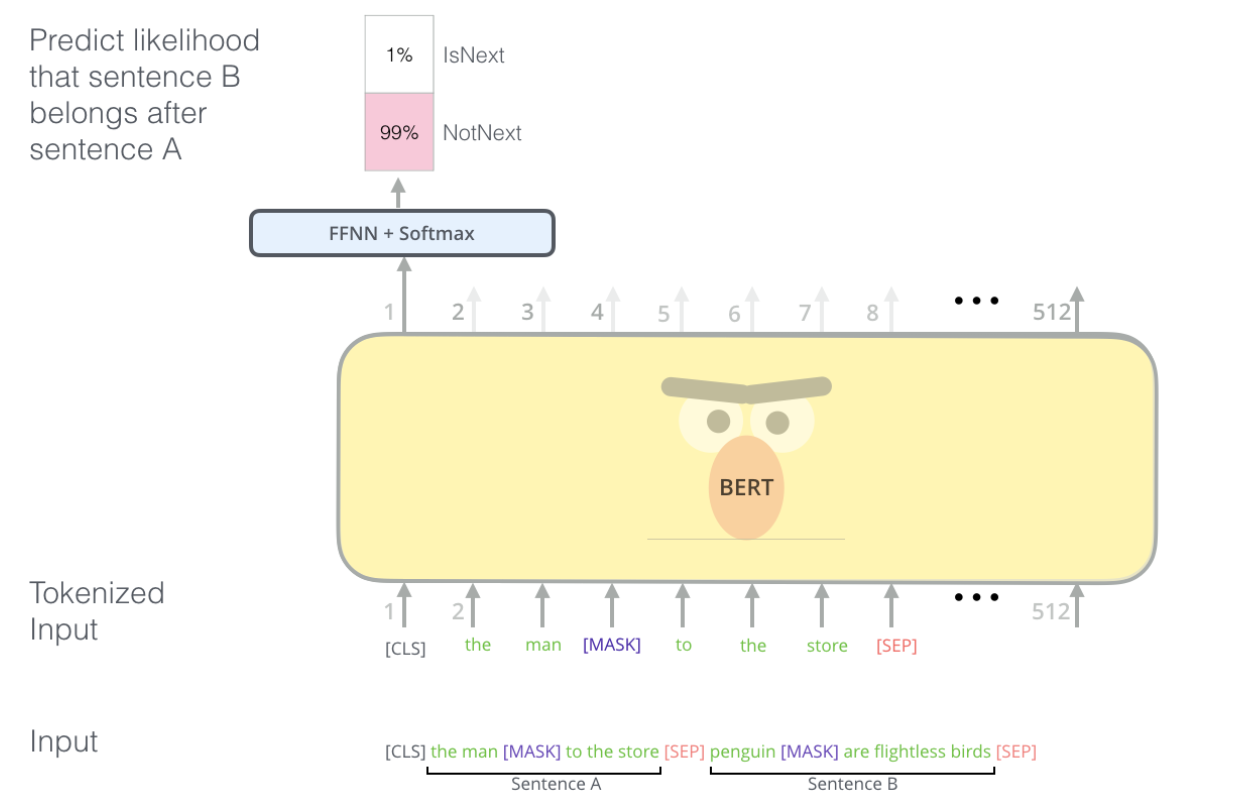
\includegraphics[width = 8.50cm]{figure/bert-nsp.png}\\ 
		\citebutton{Source: Jay Alammar}{https://jalammar.github.io/illustrated-bert/}
	\end{figure}

\vfill

\end{frame}

% ------------------------------------------------------------------------------

\begin{frame}{Pre-Training BERT}

\vfill

\textbf{Setup:}

\begin{itemize}
	\item 13 GB of text (BooksCorpus $+$ Eng. Wikipedia)\\
				$\rightarrow$ Back then: \textbf{huge}; Now: rather \textbf{small}
	\item Train for approximately* 40 epochs
	\item 4 (16) \href{https://cloud.google.com/tpu/}{Cloud TPUs} for 4 days for the BASE (LARGE) variant
	\item Loss function: $$Loss_{BERT} = Loss_{MLM} + Loss_{NSP}$$
\end{itemize}

\vfill

{\scriptsize *1.000.000 steps on batches of 256 sequences with a sequence length of 512 tokens}
\end{frame}

% ------------------------------------------------------------------------------

\begin{frame}{Pre-Training BERT}

\vfill

\textbf{Sequence lengths:}

\begin{itemize}
	\item For their experiments:
		\begin{itemize}
			\item Pre-train w/ sequence length 128 for 90\% of the steps
			\item Pre-train w/ sequence length 512 for 10\% of the steps \\
		\end{itemize}
	\item \textit{Reason:} Positional embeddings
		\begin{itemize}
			\item Learned, not sinusoidal (as opposed to the original Transformer)
			\item Training on long sequences necessary to learn them well
			\item \textbf{But:} Training expensive, hence this ``compromise``
		\end{itemize}
\end{itemize}

\vfill

\end{frame}

% ------------------------------------------------------------------------------

\begin{frame}{Fine-Tuning BERT}
	\begin{figure}
	\centering
		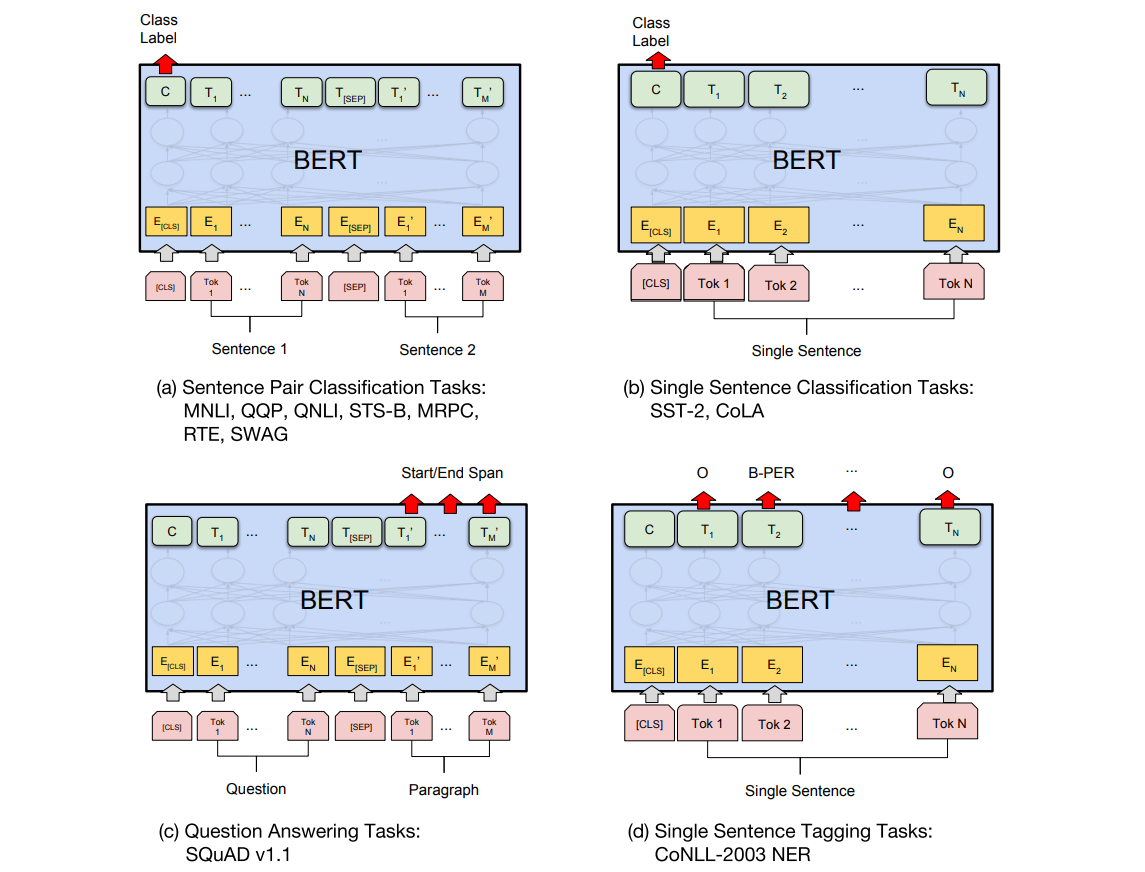
\includegraphics[width = 8.50cm]{figure/bert-finetune.png}\\ 
	\citebutton{Source: Devlin et al., 2019}{https://aclanthology.org/N19-1423.pdf}
	\end{figure}
\end{frame}


% ------------------------------------------------------------------------------

\begin{frame}{Fine-Tuning BERT}

\vspace{1.5cm}

	\begin{figure}
	\centering
		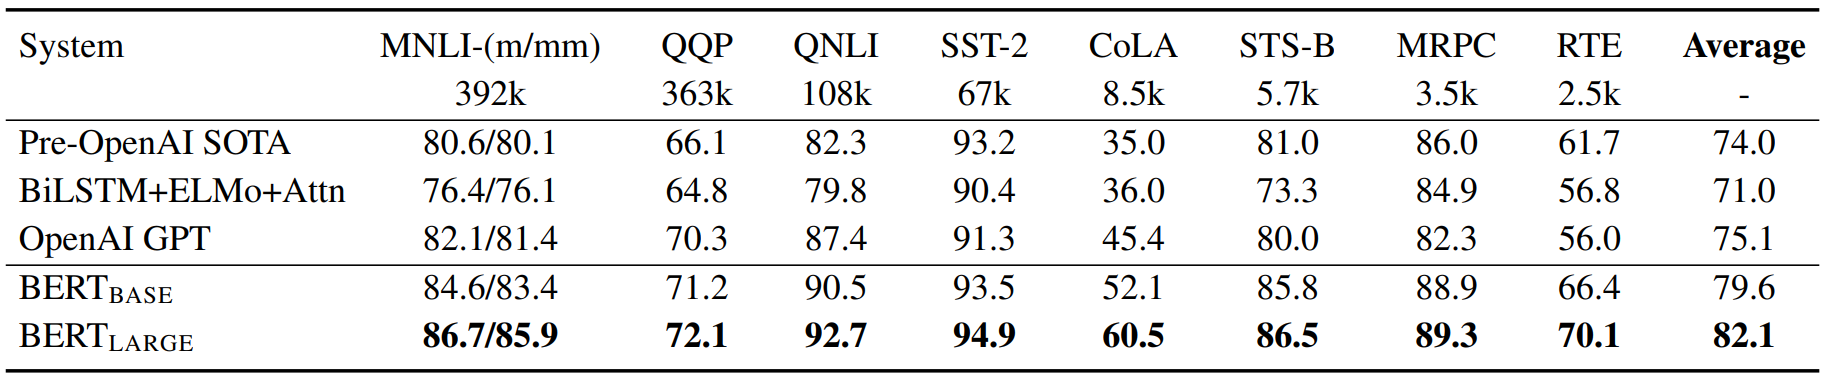
\includegraphics[width = 11cm]{figure/bert-sota.png}\\ 
	\citebutton{Source: Devlin et al., 2019}{https://aclanthology.org/N19-1423.pdf}
	\end{figure}
\begin{itemize}
	\item Performance of BERT on the GLUE Benchmark \citebutton{Wang et al., 2018}{https://gluebenchmark.com/}
	\item Beats all of the previous state-of-the-art models
	\item In the meantime: Other models (way) better than BERT
\end{itemize}

\end{frame}

% ------------------------------------------------------------------------------

\begin{frame}{Fine-tuning details}

\vfill

\begin{itemize}
	\item Relatively cheap compared to pre-training:
		\begin{itemize}
			\item $<$ 1 hour on a single Cloud TPU
			\item "a few hours" on a GPU
		\end{itemize}
	\item Recommendations for hyperparameters:
		\begin{itemize}
			\item \textbf{Batch Size:} 16, 32
			\item \textbf{Adam learning rate:} 5e-5, 3e-5, 2e-5
			\item \textbf{\#epochs:} 2, 3, 4
			\item \textbf{Dropout probability:} 0.1
		\end{itemize}
	\item Data sets w/ > 100k labeled examples rather insensitive to hyperparameters
\end{itemize}
	
\vfill

\end{frame}

% ------------------------------------------------------------------------------

\begin{frame}{Feature Extraction from BERT}

\vfill

	\begin{figure}
		\centering
		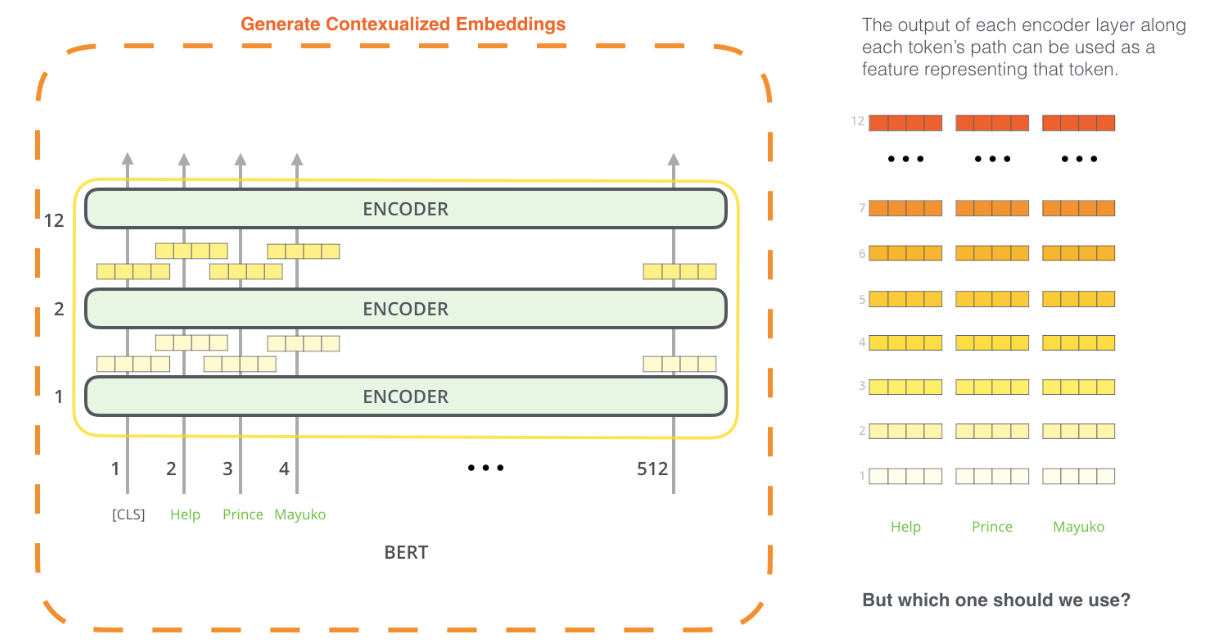
\includegraphics[width = 11cm]{figure/bert-featextr.png}\\ 
		\citebutton{Source: Jay Alammar}{https://jalammar.github.io/illustrated-bert/}
	\end{figure}

\vfill

\end{frame}

% ------------------------------------------------------------------------------

\begin{frame}{Feature Extraction from BERT}

	\begin{figure}
	\centering
		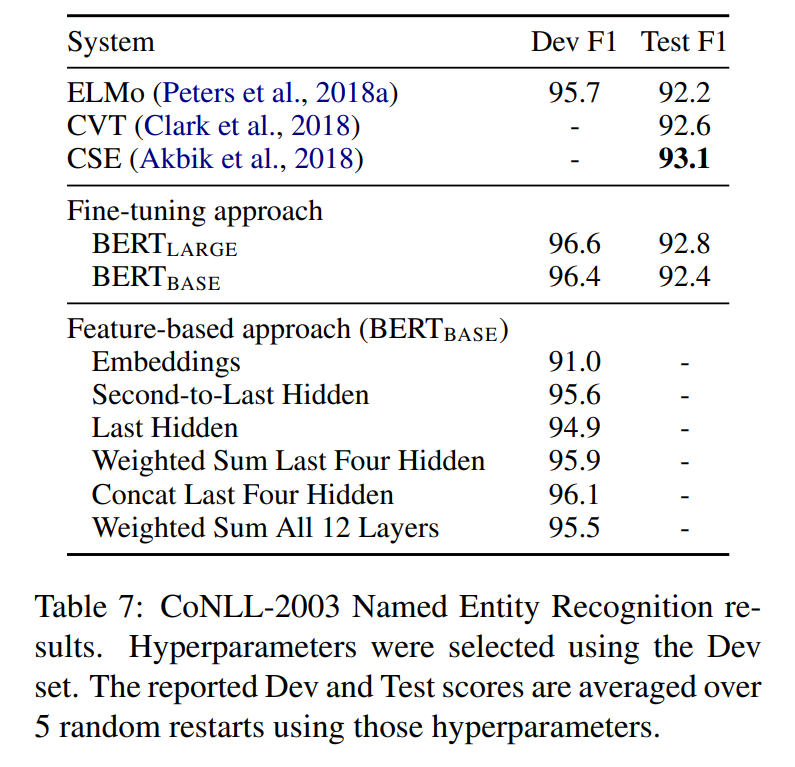
\includegraphics[width = 6.38cm]{figure/bert-featextr-results.png}\\ 
	\citebutton{Source: Devlin et al., 2019}{https://aclanthology.org/N19-1423.pdf}
	\end{figure}

\end{frame}

% ------------------------------------------------------------------------------


%%%%%%%%%%%%%%%%%%%%%%%%%%%%%%%%%%%%%%%%%%%%%%%%%%%%%%%%%%%%%%%%%%
\section{Basic definitions and challenges}
% Source: DL4NLP chapter04-bert/slides-45-transferlearning-selfsup.tex
%%%%%%%%%%%%%%%%%%%%%%%%%%%%%%%%%%%%%%%%%%%%%%%%%%%%%%%%%%%%%%%%%%
% ------------------------------------------------------------------------------

\begin{frame}{feature-based transfer learning}

\vfill

	\textbf{How it works with word2vec:}
	
	\begin{itemize}
		\item Train word2vec on some "fake task" (CBOW or Skip-gram)
		\item Extract the stored knowledge (a.k.a. embedding)\\
					\textit{or:} Directly download embeddings from the web 
		\item Perform a different (supervised) task using the embeddings
	\end{itemize}
	
	\vspace{.3cm}
	
	\textbf{How it works with ELMo:}
	
	\begin{itemize}
		\item Do not \textit{extract} the stored knowledge, but use the whole embedding model \textit{as is}
		\item Only train/fine-tune task specific weights on top of ELMo
	\end{itemize}
	
\vfill

\end{frame}

% ------------------------------------------------------------------------------

\begin{frame}{fine-tuning transfer learning}

\vfill

	\textbf{How it works with BERT:}
	
	\begin{itemize}
		\item Train BERT via masked language modeling
		\item Fine-tune selected parts of the model using labeled data
	\end{itemize}
	
	\vspace{.3cm}
	
	\textbf{Feature-based alternative:}
	
	\begin{itemize}
		\item \textit{Extract} the embeddings and use them for, e.g., a classification task
		\item \textit{Freeze} the model, fine-tune only classification head
	\end{itemize}
	
\vfill

\end{frame}

% ------------------------------------------------------------------------------

\begin{frame}{Taxonomy of transfer learning \href{https://ruder.io/thesis/}{\beamergotobutton{Ruder, 2019}}}
	\begin{figure}
		\centering
		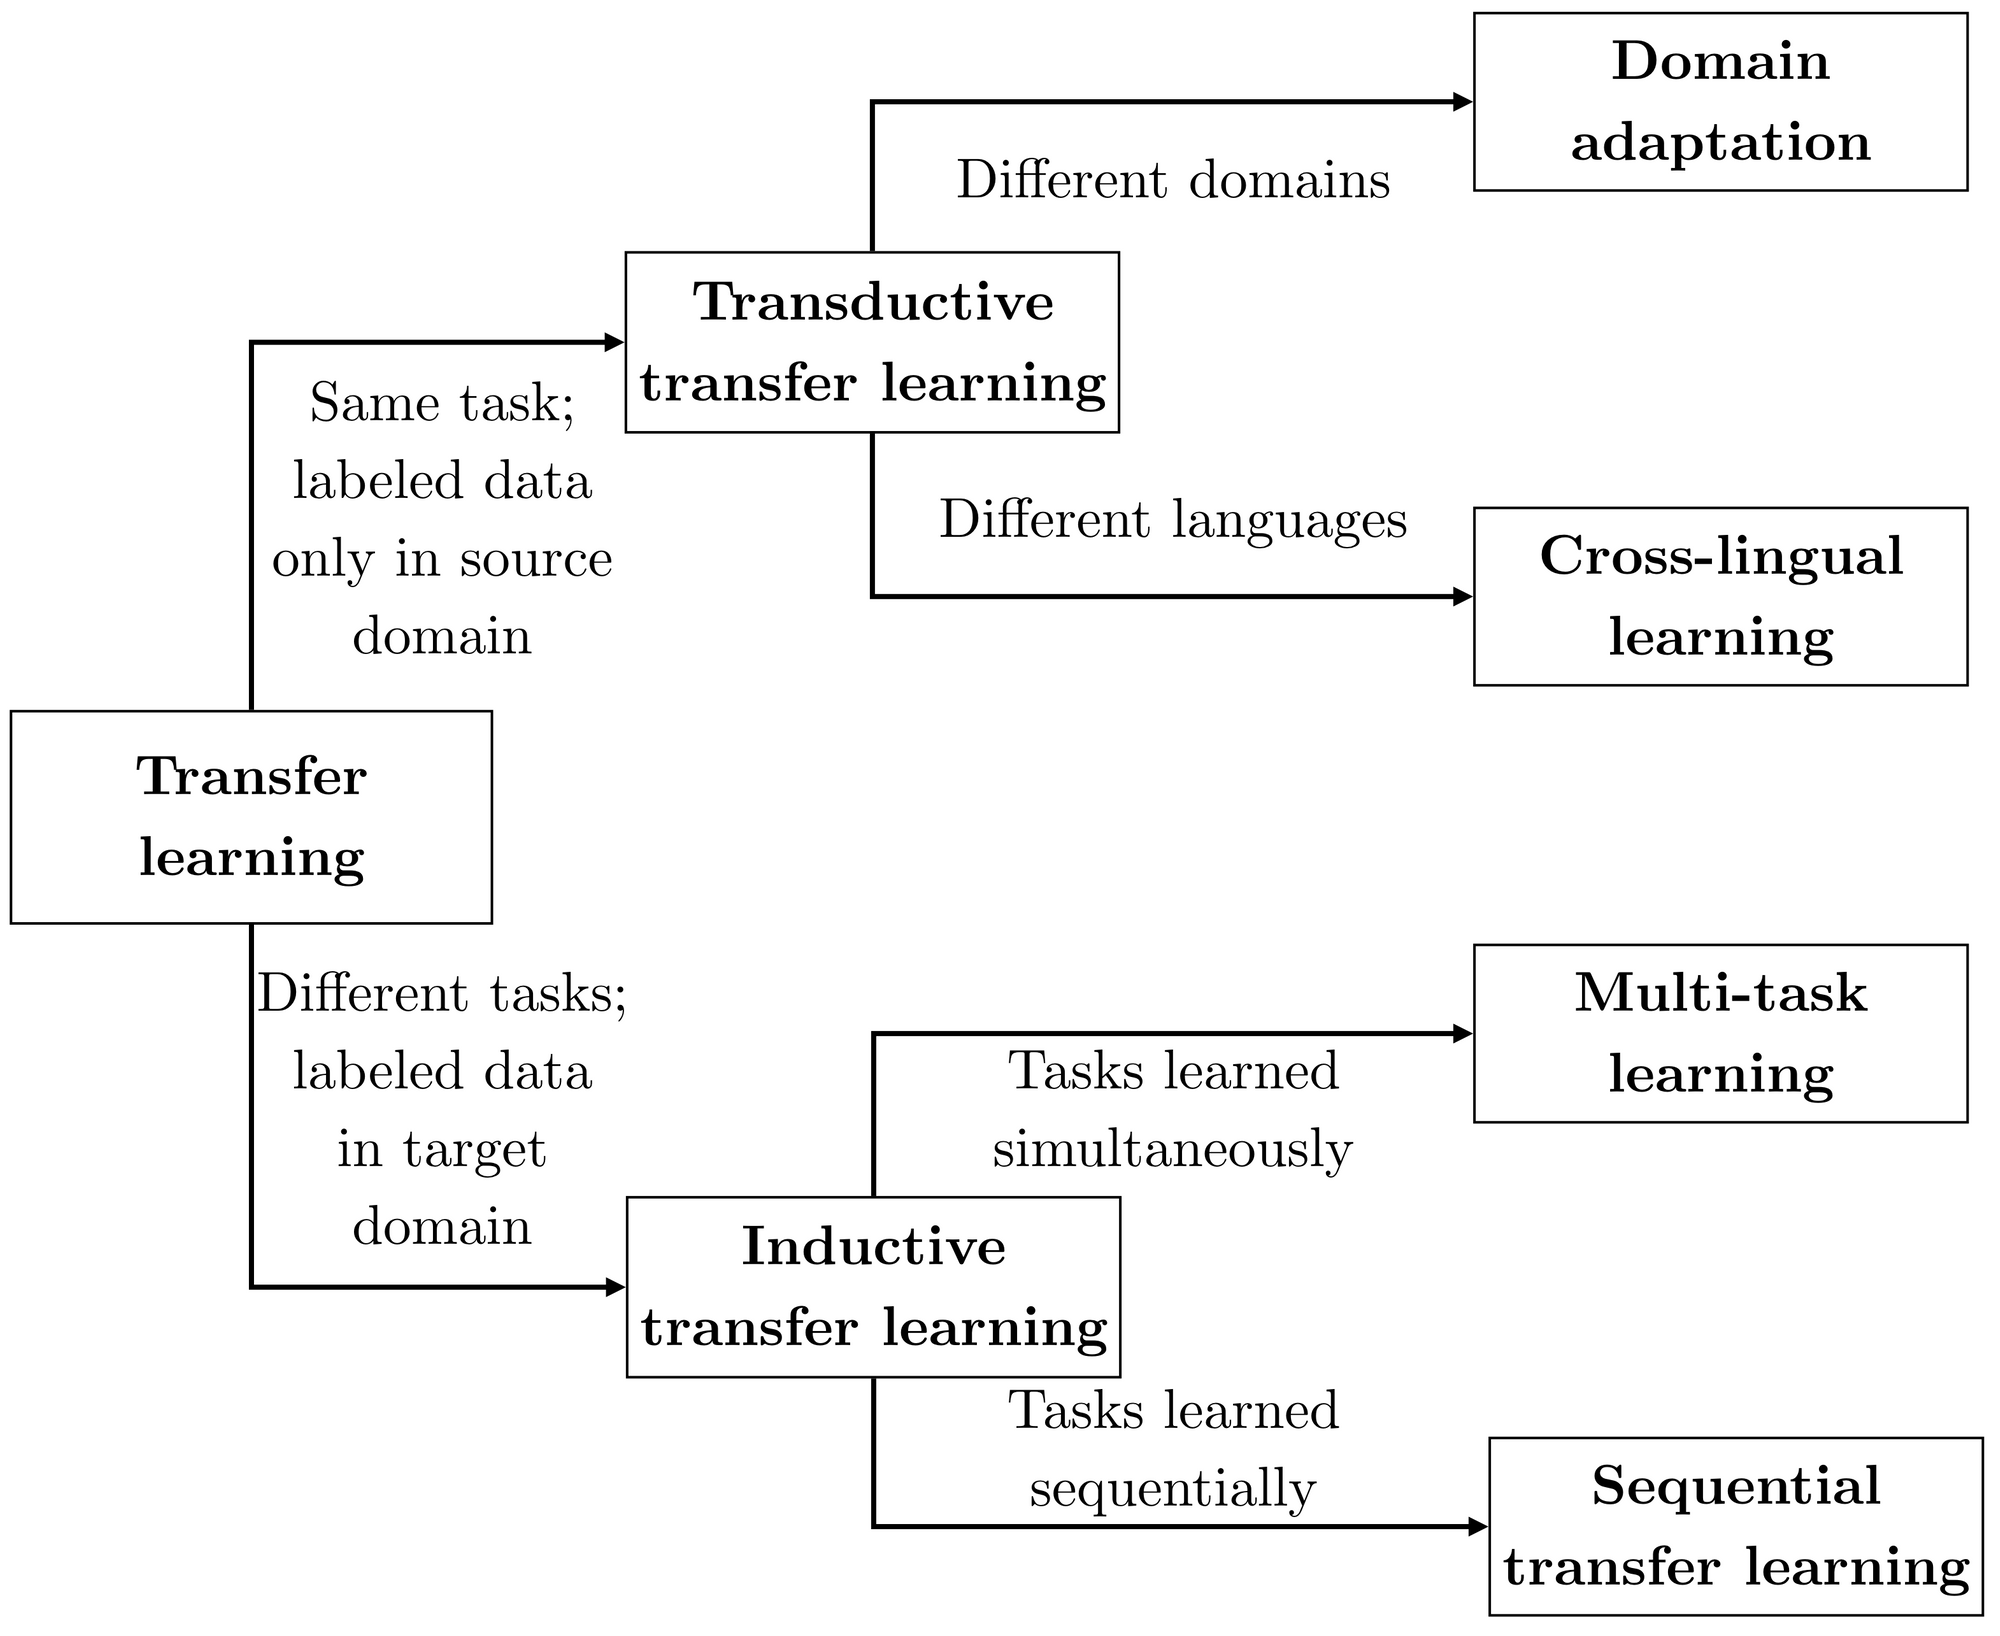
\includegraphics[width = 6.80cm]{figure/transfer_learning_taxonomy-1.png}\\ 
		\footnotesize{Source:} \href{https://ruder.io/thesis/}{\footnotesize \it Sebastian Ruder}
	\end{figure}
\end{frame}

% ------------------------------------------------------------------------------

\begin{frame}{Taxonomy of transfer learning \href{https://ruder.io/thesis/}{\beamergotobutton{Ruder, 2019}}}

\vfill

	\textbf{Transductive Transfer learning}

	\begin{itemize}
		\item Domain adaptation:\\
					$\rightarrow$ "\textit{Transfer knowledge learned from performing task A on labeled data from domain X to performing task A in domain Y.}"\\\mbox{}
		\item Cross-lingual learning:\\
					$\rightarrow$ "\textit{Transfer knowledge learned from performing task A on labeled data from language X to performing task A in language Y.}"\\\mbox{}
		\item \textit{Important:} No labeled data in target domain/language \textit{Y}.
	\end{itemize}
	
\vfill

\end{frame}

% ------------------------------------------------------------------------------

\begin{frame}{Taxonomy of transfer learning \href{https://ruder.io/thesis/}{\beamergotobutton{Ruder, 2019}}}

\vfill

	\textbf{Inductive Transfer learning}

	\begin{itemize}
		\item Multi-task learning:\\
					$\rightarrow$ "\textit{Transfer knowledge learned from performing task A on data from domain X to performing multiple (simultaneous) tasks B, C, D, .. in domain Y.}"\\\mbox{}
		\item Sequential transfer learning:\\
					$\rightarrow$ "\textit{Transfer knowledge learned from performing task A on data from domain X to performing multiple (sequential) tasks B, C, D, .. in domain Y.}"\\\mbox{}
		\item \textit{Important:} Labeled data only for task(s) from target domain \textit{Y}.
	\end{itemize}
	
\vfill

\end{frame}

% ------------------------------------------------------------------------------

\begin{frame}{remark on multilinguality}

\vfill

\textbf{Cross-lingual transfer:}

\begin{itemize}
	\item Languages can be grouped into certain families
	\item Patterns that a model learns for one language, might be beneficial for learning a second language 
				(just as it is for us humans as well: For those who learned French in high school, learning Spanish
				afterwards might be easier)
	\item Again: Scarcity of resources; assume the following scenario:
		\begin{itemize}
			\item \textbf{Large} parallel corpus for languages A and B
			\item \textbf{Large} parallel corpus for languages A and C
			\item \textit{Small} parallel corpus for languages B and C
			\item[$\to$] Training a model for B and C in isolation not the best idea
		\end{itemize}
\end{itemize}

\vfill

\end{frame}

% ------------------------------------------------------------------------------

\begin{frame}{key component: self-supervision}

\vfill

	\begin{figure}
		\centering
		
\includegraphics[width=10cm]{figure/selfsup.jpeg}
	\end{figure}
	
\vfill

\end{frame}

% ------------------------------------------------------------------------------

\begin{frame}{Definition: self-supervision}

	\vfill 
	
	\textit{Unsupervised Learning:}

	\begin{itemize}
		\item No labels attached to the data
		\item Learn patterns / clusters from the features only
	\end{itemize}
	
	\textit{Supervised Learning:}

	\begin{itemize}
		\item (Gold) Labels attached to the data
		\item Learn from the association between features and labels
	\end{itemize}
	
	\textbf{Self-Supervised Learning:}

	\begin{itemize}
		\item No \textit{external} labels attached to the data\\
					$\to$ Samples with suitable labels can be generated from the known structure of the data itself 
		\item \textit{Technically} supervised learning, but \textit{no labeling effort} $+$ simultan-\\eous ability to generate massive amounts of labeled data points
	\end{itemize}
	
	\vfill 
	
\end{frame}

% ------------------------------------------------------------------------------

\begin{frame}{Self-supervised objectives}

\vfill

\textbf{Recap: Language modeling}
	
	\begin{itemize}
		\item \textit{Training objective:} Given a context, predict the next word
	\end{itemize}
	
\begin{block}{Illustration (context size $=$ 2)}
\begin{tabular}{|c|c|c|cccccc|}
\hline
\cellcolor{blue!15}The & \cellcolor{blue!65}quick & brown & fox & jumps & over & the & lazy & dog \\
\hline
\end{tabular}\\
$\Rightarrow$ \quad (the, quick)
\begin{tabular}{|c|c|c|c|ccccc|}
\hline
\cellcolor{blue!15}The & \cellcolor{blue!15}quick & \cellcolor{blue!65}brown & fox & jumps & over & the & lazy & dog \\
\hline
\end{tabular}\\
$\Rightarrow$ \quad ([the, quick], brown)
\begin{tabular}{|c|c|c|c|ccccc|}
\hline
The & \cellcolor{blue!15}quick & \cellcolor{blue!15}brown & \cellcolor{blue!65}fox & jumps & over & the & lazy & dog \\
\hline
\end{tabular}\\
$\Rightarrow$ \quad ([quick, brown], fox)
\begin{tabular}{|c|c|c|c|ccccc|}
\hline
The & quick & \cellcolor{blue!15}brown & \cellcolor{blue!15}fox & \cellcolor{blue!65}jumps & over & the & lazy & dog \\
\hline
\end{tabular}\\
$\Rightarrow$ \quad ([brown, fox], jumps)
\end{block}
	
\vfill

\end{frame}

% ------------------------------------------------------------------------------

\begin{frame}{Self-supervised objectives}

\vfill

\textbf{Recap: Skip-gram}
	
	\begin{itemize}
		\item \textit{Training objective:} Given a word, predict the neighbouring words
    \item \textit{Generation of samples:} Sliding fixed-size window over the text
	\end{itemize}
	
\begin{block}{Illustration}
\begin{tabular}{|c|c|c|cccccc|}
\hline
\cellcolor{blue!15}The & \cellcolor{blue!65}quick & \cellcolor{blue!65}brown & fox & jumps & over & the & lazy & dog \\
\hline
\end{tabular}\\
$\Rightarrow$ \quad (the, quick); (the, brown)
\begin{tabular}{|c|c|c|c|ccccc|}
\hline
\cellcolor{blue!65}The & \cellcolor{blue!15}quick & \cellcolor{blue!65}brown & \cellcolor{blue!65}fox & jumps & over & the & lazy & dog \\
\hline
\end{tabular}\\
$\Rightarrow$ \quad (quick, the); (quick, brown); (quick, fox)
\begin{tabular}{|c|c|c|c|ccccc|}
\hline
\cellcolor{blue!65}The & \cellcolor{blue!65}quick & \cellcolor{blue!15}brown & \cellcolor{blue!65}fox & \cellcolor{blue!65}jumps & over & the & lazy & dog \\
\hline
\end{tabular}\\
$\Rightarrow$ \quad (brown, the); (brown, quick); (brown, fox); (brown, blue)
\begin{tabular}{|c|c|c|c|ccccc|}
\hline
The & \cellcolor{blue!65}quick & \cellcolor{blue!65}brown & \cellcolor{blue!15}fox & \cellcolor{blue!65}jumps & \cellcolor{blue!65}over & the & lazy & dog \\
\hline
\end{tabular}\\
$\Rightarrow$ \quad (fox, quick); (fox, brown); (fox, jumps); (fox, over)
\end{block}
	
\vfill

\end{frame}

% ------------------------------------------------------------------------------

\begin{frame}{Self-supervised objectives}

\vfill

\textbf{Self-supervised objectives:}
	
	\begin{itemize}
		\item Skip-gram objective (cf. word2vec \citebutton{Mikolov et al., 2013}{https://arxiv.org/pdf/1301.3781.pdf})
		\item Language modeling objective (cf. e.g. \citebutton{Bengio et al., 2003}{http://www.jmlr.org/papers/volume3/bengio03a/bengio03a.pdf})
		\item \textit{Masked language modeling (MLM)} objective (cf. BERT)\\
					$\rightarrow$ Replace words by a \texttt{[MASK]} token and train the model to predict
	\end{itemize}
	
\textbf{Other examples:}
	
	\begin{itemize}
		\item \textit{Permutation language modeling (PLM)} objective \citebutton{Yang et al., 2019}{https://papers.nips.cc/paper/8812-xlnet-generalized-autoregressive-pretraining-for-language-understanding.pdf}\\
					$\rightarrow$ Autoregressive objective of XLNet
		\item \textit{Replaced token detection} (RTD) objective \citebutton{Clark et al, 2020}{https://arxiv.org/pdf/2003.10555.pdf}\\
					$\rightarrow$ Requires two models: One performing MLM \& the second model to discriminate between actual and the predicted tokens
	\end{itemize}
	
\vfill

\end{frame}

% ------------------------------------------------------------------------------


%%%%%%%%%%%%%%%%%%%%%%%%%%%%%%%%%%%%%%%%%%%%%%%%%%%%%%%%%%%%%%%%%%
\section{Implications for Future Work \& BERTology}
% Source: DL4NLP chapter05-bert-based/slides-51-bertology.tex
%%%%%%%%%%%%%%%%%%%%%%%%%%%%%%%%%%%%%%%%%%%%%%%%%%%%%%%%%%%%%%%%%%
% ------------------------------------------------------------------------------

\begin{frame}{Implications / Limitations}

\vfill

	\begin{itemize}
		\item BERT changed the way NLP research was done over night\\
					(probably as impactful as ChatGPT in 2022, but not so incredibly hyped in the general public)
		\item This paradigm change had several \myblue{implications} on how research was done in the ``Post-BERT era``
		\item It also came with several \myblue{limitations} that are still to be solved or have been solved already
		\item Computational power also became an important issue, but this will not be stressed as much in this chapter
	\end{itemize}

\vfill

\end{frame}

% ------------------------------------------------------------------------------

\begin{frame}{(1) language diversity}

\vfill

	\begin{itemize}
		\item BERT trained on a corpus of English text
		\item More importantly: Also only evaluated on English benchmarks (obviously)
					\citebutton{GLUE}{https://gluebenchmark.com/}
					\citebutton{SQUAD}{https://rajpurkar.github.io/SQuAD-explorer/}
					\citebutton{RACE}{https://www.qizhexie.com/data/RACE_leaderboard.html}
		\item Devlin et al. (2019) published different (monolingual) models, but only varying in size, not in language
		\item Later: Multilingual BERT model \citebutton{mBERT}{https://github.com/google-research/bert/blob/master/multilingual.md} for 100+ languages
		\item This leads to a shared embedding space for all the languages included in the model
		\item Before this: Need for alignment of separately learned embedding spaces
	\end{itemize}

\vfill

\end{frame}

% ------------------------------------------------------------------------------

\begin{frame}{(1) language diversity}

\vfill

\begin{itemize}
	\item The breakthrough performance of BERT in the English language triggered a wave of new
				BERT models in different languages. Just to name a few:
			\begin{itemize}
				\item \citebutton{German BERT}{https://huggingface.co/bert-base-german-cased}
				\item \citebutton{FlauBERT (French)}{https://huggingface.co/flaubert/flaubert_base_cased}
				\item \citebutton{BETO (Spanish)}{https://huggingface.co/dccuchile/bert-base-spanish-wwm-cased}
				\item \citebutton{BERTje (Dutch)}{https://huggingface.co/GroNLP/bert-base-dutch-cased}
				\item \citebutton{Chinese BERT}{https://huggingface.co/bert-base-chinese}
				\item \citebutton{RuBERT (Russian)}{https://huggingface.co/DeepPavlov/rubert-base-cased}
				\item \citebutton{Italian BERT}{https://huggingface.co/dbmdz/bert-base-italian-cased}
				\item ...
			\end{itemize}
\end{itemize}
	
\vfill

\end{frame}

% ------------------------------------------------------------------------------

\begin{frame}{(2) pretrain-finetune + transformer}

\vfill

\textbf{Before BERT:} 
			\begin{itemize}
				\item ELMo (and other specialized architectures) very popular
				\item Examples (also CNNs): 
							\citebutton{Kim, 2014}{https://arxiv.org/abs/1408.5882}
							\citebutton{Zhang et al., 2016}{https://proceedings.neurips.cc/paper/2015/file/250cf8b51c773f3f8dc8b4be867a9a02-Paper.pdf}
			\end{itemize}
\textbf{After BERT:}
			\begin{itemize}
				\item Using a pre-trained model and fine-tuning it to one's own data is* the de-facto standard
				\item CNNs and RNNs rarely used, different variants of the transformer or other self-attention based mechanisms are the backbone of nearly every architecture
			\end{itemize}

\vfill

{\scriptsize *Or probably ``\textit{was}``. This standard is (rapidly) changing at the moment as Large Language Models (LLMs) and Prompting are becoming incredibly popular and effective.}
\end{frame}

% ------------------------------------------------------------------------------

\begin{frame}{(3) pretrain-finetune discrepancy}

\vfill

	\begin{itemize}
		\item BERT \textit{artificially} introduces \texttt{[MASK]} tokens during pre-training
		\item \texttt{[MASK]}-token does not occur during fine-tuning\\
					$\rightarrow$ Lacks the ability to model joint probabilities\\
					$\rightarrow$ Assumes independence of predicted tokens (given the context)
		\item Other pre-training objectives (e.g. language modeling) don't have this issue
		\item Further: BERT only learns from predicting the 15\% tokens which are \texttt{[MASK]}ed (or randomly replaced / kept as is)
	\end{itemize}

\vfill

\end{frame}

% ------------------------------------------------------------------------------

\begin{frame}{(4) independence assumption}

\vspace{1.5cm}

\textbf{\texttt{[MASK]-ing procedure}:}

\begin{itemize}
	\item "Given a sentence, predict \texttt{[MASK]}ed tokens"
	\item All \texttt{[MASK]}ed tokens are predicted based on the un-\texttt{[MASK]}ed tokens
	\item \textit{Implicit assumption:} Independence of \texttt{[MASK]}ed tokens
\end{itemize}

	\begin{figure}
		\centering
		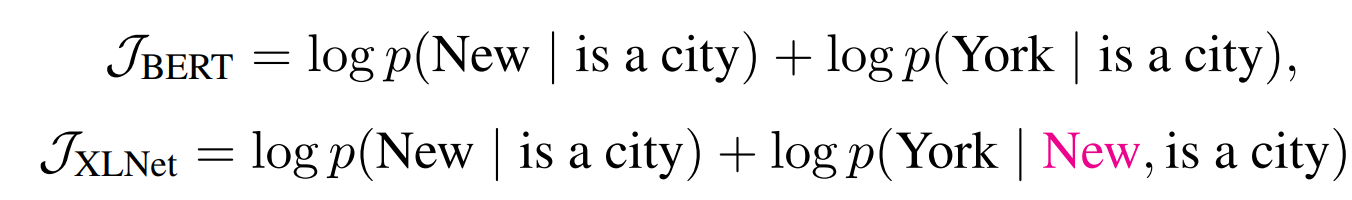
\includegraphics[width = 9cm]{figure/xlnet-objective}\\ 
		{\tiny Prediction of [New, York] given the factorization order [is, a, city, New, York]}\\
		\citebutton{Source: Yang et al., 2019}{https://papers.nips.cc/paper_files/paper/2019/hash/dc6a7e655d7e5840e66733e9ee67cc69-Abstract.html}
	\end{figure}
	
\end{frame}

% ------------------------------------------------------------------------------

\begin{frame}{(5) maximum sequence length}

\begin{figure}
\centering
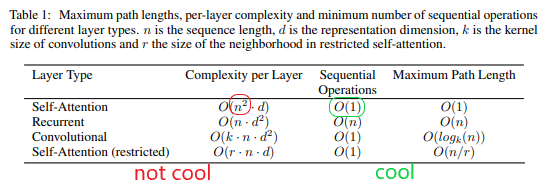
\includegraphics[width = 7.22cm]{figure/bert-problem.png}\\ 
	\beamergotobutton{\href{https://arxiv.org/abs/1706.03762}{Source: Vaswani et al., 2017}}
\end{figure}

\textbf{Limitation:}

\begin{itemize}
	\item BERT can only consume sequences of up to 512 tokens
	\item Two sentences for NSP are sampled such that $$length_{sentence A} + length_{sentence B} \leq 512$$
	\item Reason: Computational complexity of Transformer scales quadratically with the sequence length\\
				$\rightarrow$ Longer sequences are disproportionally expensive
\end{itemize}

\end{frame}

% ------------------------------------------------------------------------------

\begin{frame}{(6) bias}

\vfill

\begin{itemize}
	\item Already known to exist in static pre-trained embeddings:
	\item[] \textit{Man is to Computer Programmer as Woman is to Homemaker? Debiasing Word Embeddings} \citebutton{Bolukbasi et al., 2016}{https://arxiv.org/abs/1607.06520}
	\item BERT also learns the patterns from the data it is trained on
	\item Research on Detecting/Mitigating Bias receives a lot of attention
\end{itemize}


\vfill

\end{frame}

% ------------------------------------------------------------------------------

\begin{frame}{(6) bias -- example}

\vfill

\begin{itemize}
	\item \citebutton{Nadeem et al., 2021}{https://aclanthology.org/2021.acl-long.416.pdf} create a data set for measuring bias in LMs
	\item Four categories: Gender, Profession, Race, Religion
	\item Two types of probes: Intra- and Inter-sentence test sets
\end{itemize}

\begin{figure}%
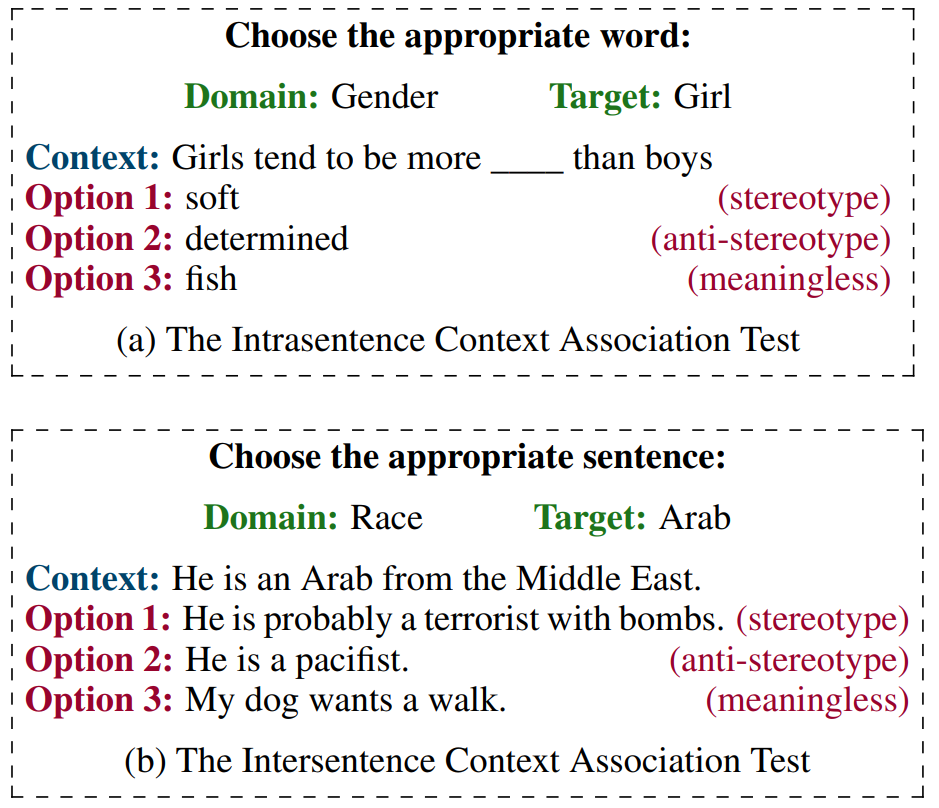
\includegraphics[width=6cm]{figure/stereoset.png}%
\end{figure}

\vfill

\end{frame}

% ------------------------------------------------------------------------------

\begin{frame}{(6) bias -- example}

\vfill

\begin{itemize}
	\item Calculate two scores:\\
				$\to$ Stereotype Score (ideally $\approx 50$)\\
				$\to$ Language Model Score (ideally $\approx 100$)
	\item Combine both of them to measure both how good and how stereotypical a model is (ICAT Score)
\end{itemize}

\begin{figure}%
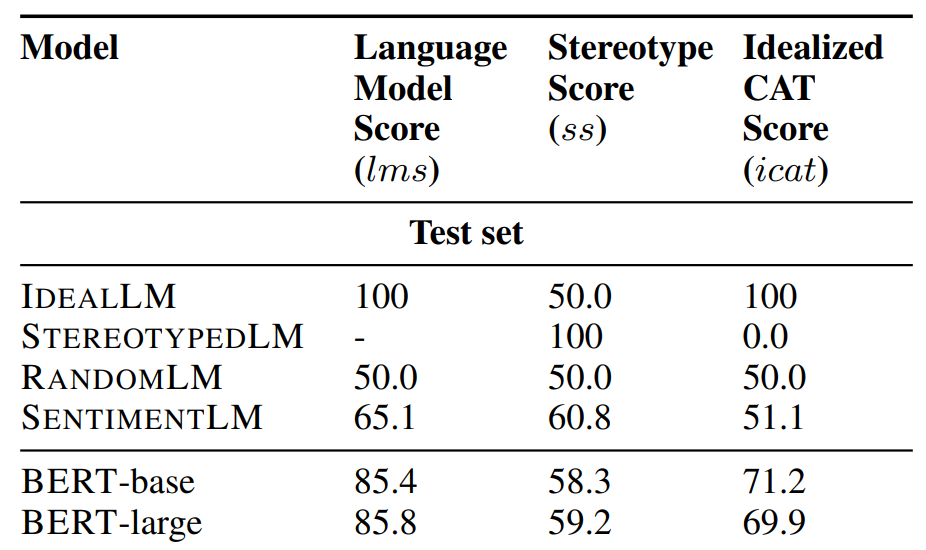
\includegraphics[width=7cm]{figure/stereoset2.png}%
\end{figure}

\vfill

\end{frame}

% ------------------------------------------------------------------------------

\begin{frame}{BERTology}

\vfill

\textbf{Origin}

\begin{itemize}
		\item Survey by \citebutton{Rodgers et al., 2020}{https://aclanthology.org/2020.tacl-1.54.pdf} covering studies on BERT coined the term ``BERTology``.
		\item \citebutton{Huggingface}{https://huggingface.co/docs/transformers/bertology} defines it as ``\textit{field of study concerned with investigating the inner working of large-scale transformers like BERT}``
\end{itemize}

\textbf{Included investigations} \citebutton{Rodgers et al., 2020}{https://aclanthology.org/2020.tacl-1.54.pdf}
	
\begin{itemize}
		\item Does BERT exhibit Syntactic/Semantic/World knowledge?
		\item Localization of Linguistic knowledge
		\item The optimal parametrization and training of BERT, i.e., number of heads, batch sizes, pre-training objectives
				\item Model compression techniques
\end{itemize}
	
\vfill

\end{frame}

% ------------------------------------------------------------------------------

\begin{frame}{(1) examining attention patterns}

\vfill

\textbf{What does BERT look at?} \citebutton{Clark et al., 2019}{https://aclanthology.org/W19-4828/}

	\begin{figure}
		\centering
		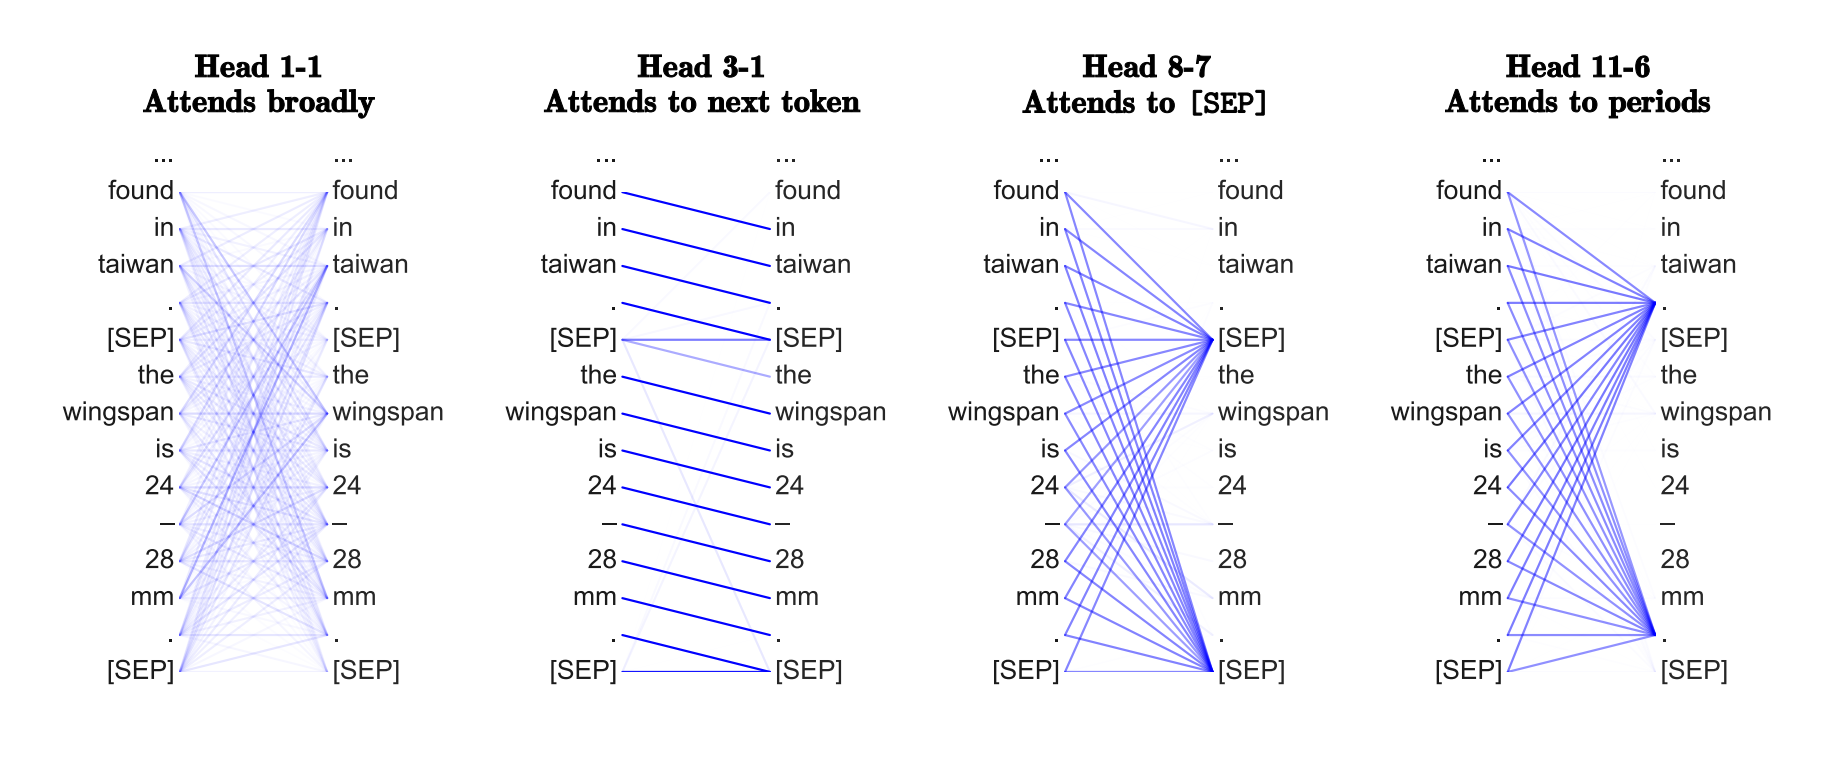
\includegraphics[width = 10cm]{figure/51-what-bert-look-at.png}
	\end{figure}
	
	\begin{itemize}
		\item Extract BERT's attention maps for 1000 segments from Wikipedia\\
					(max. segment length of 128 $\approx$ 2 paragraphs)
		\item[] $\to$ \texttt{ [CLS]<paragraph-1>[SEP]<paragraph-2>[SEP]}
	\end{itemize}
	
\vfill

\end{frame}

% ------------------------------------------------------------------------------

\begin{frame}{(1) examining attention patterns}

\vfill

\textbf{What does BERT look at?} \citebutton{Clark et al., 2019}{https://aclanthology.org/W19-4828/}

\begin{minipage}{.49\textwidth}
	\begin{figure}
		\centering
		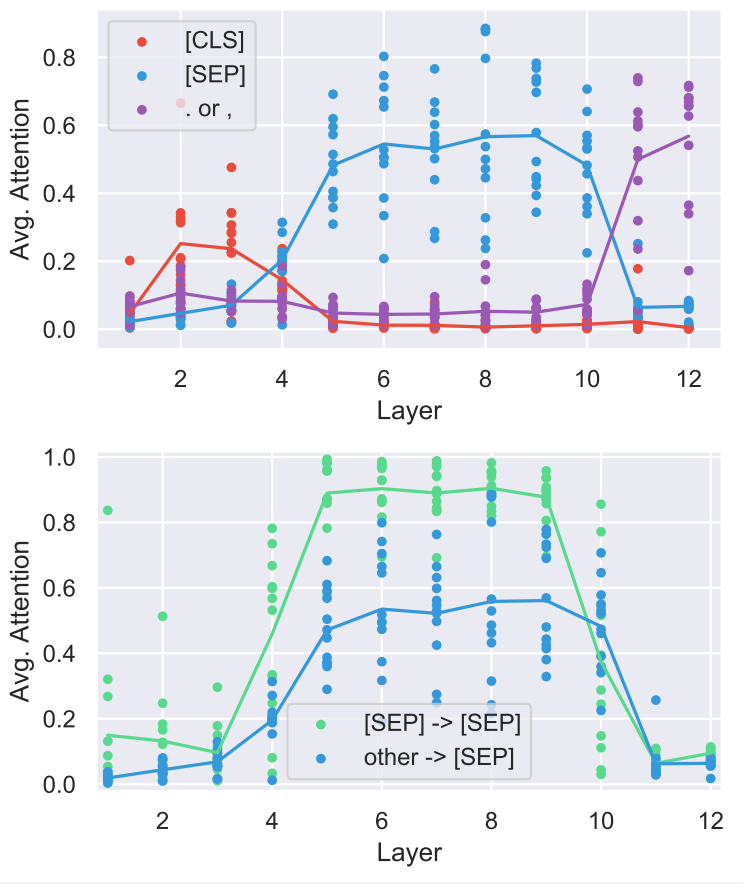
\includegraphics[width = 4cm]{figure/51-special-tokens.png}
	\end{figure}
\end{minipage}%
\begin{minipage}{.49\textwidth}
	\begin{figure}
		\centering
		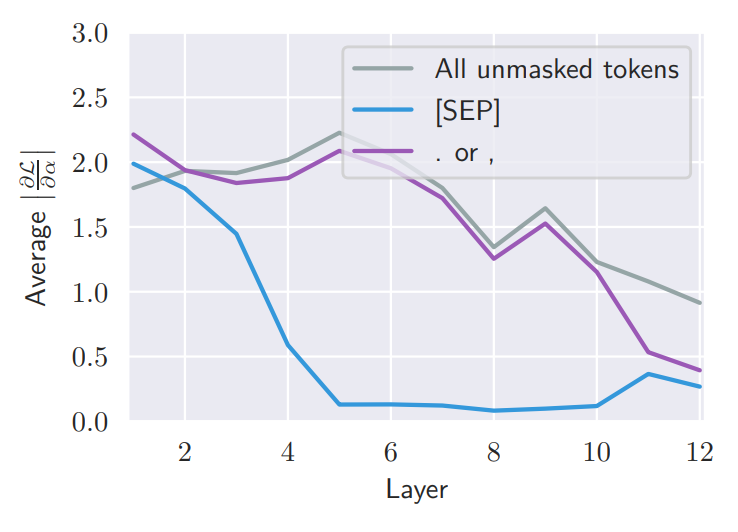
\includegraphics[width = 4cm]{figure/51-featimp.png}\\
		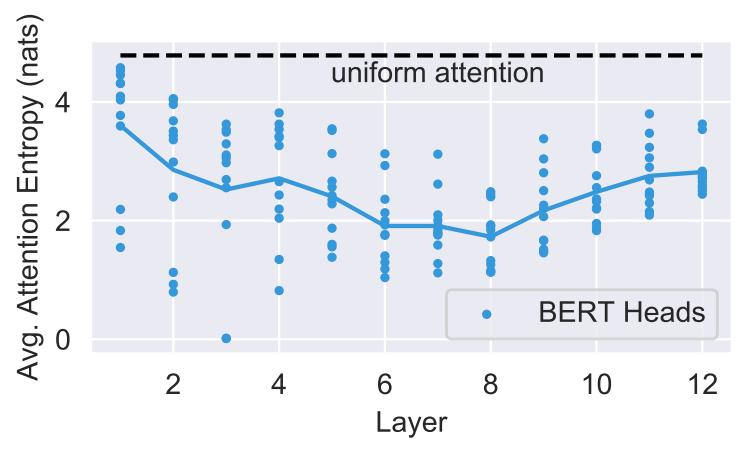
\includegraphics[width = 4cm]{figure/51-attn-entropy.png}
	\end{figure}
\end{minipage}
	
\begin{itemize}
		\item \textbf{Left:} Average Attention to special tokens
		\item \textbf{Right:} Gradient-based feature imp. (top) and Entropy (bottom)
\end{itemize}
	
\vfill

\end{frame}

% ------------------------------------------------------------------------------

\begin{frame}{(1) examining attention patterns}

\vfill

\textbf{What does BERT look at?} \citebutton{Clark et al., 2019}{https://aclanthology.org/W19-4828/}

	\begin{figure}
		\centering
		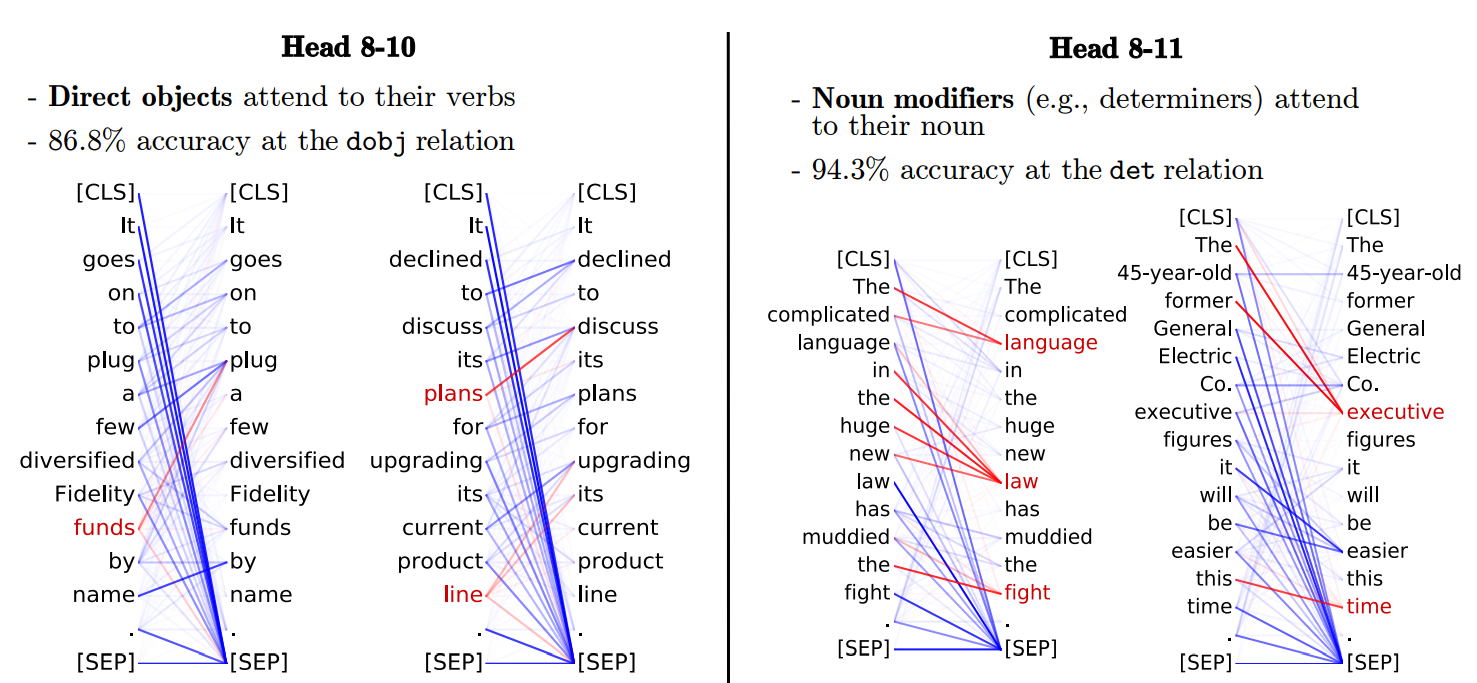
\includegraphics[width = 10cm]{figure/51-linguistic.png}
	\end{figure}
	
	\begin{itemize}
		\item \textbf{Data:} Wall Street Journal portion of the Penn Treebank\\
					(annotated with Stanford Dependencies)
	\end{itemize}
	
\vfill

\end{frame}

% ------------------------------------------------------------------------------

\begin{frame}{(2) inspecting different heads}

\vfill

\textbf{Are Sixteen Heads Really Better than One?} \citebutton{Michel et al., 2019}{https://papers.nips.cc/paper_files/paper/2019/hash/2c601ad9d2ff9bc8b282670cdd54f69f-Abstract.html}

	\begin{figure}
		\centering
		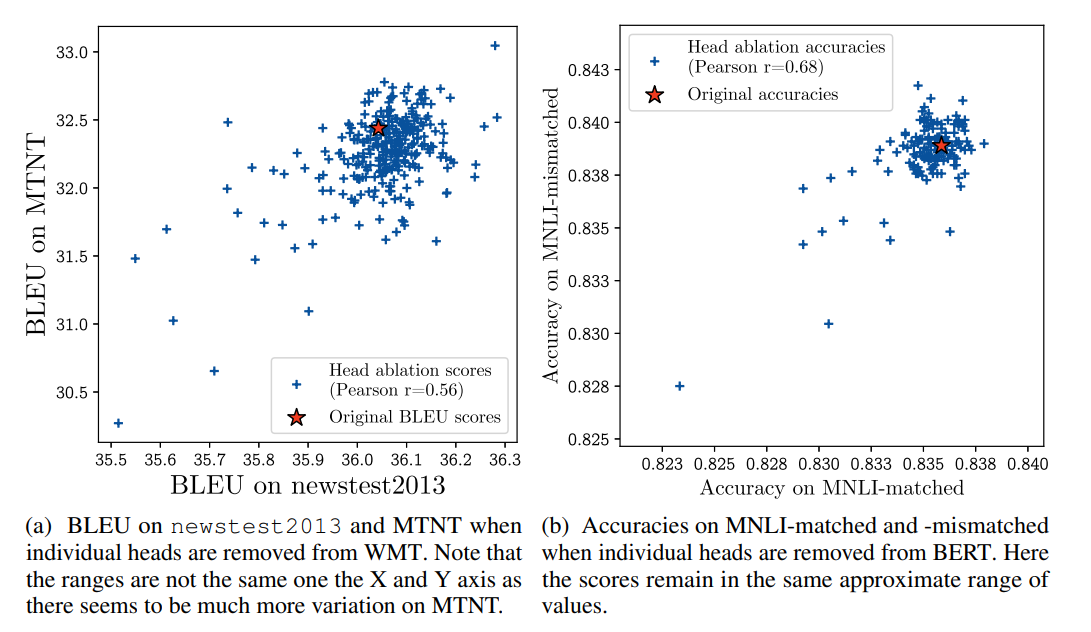
\includegraphics[width = 9.35cm]{figure/51-remove-heads.png}
	\end{figure}
	
\vfill

\end{frame}

% ------------------------------------------------------------------------------

\begin{frame}{(2) inspecting different heads}

\vfill

\textbf{Are Sixteen Heads Really Better than One?} \citebutton{Michel et al., 2019}{https://papers.nips.cc/paper_files/paper/2019/hash/2c601ad9d2ff9bc8b282670cdd54f69f-Abstract.html}

	\begin{figure}
		\centering
		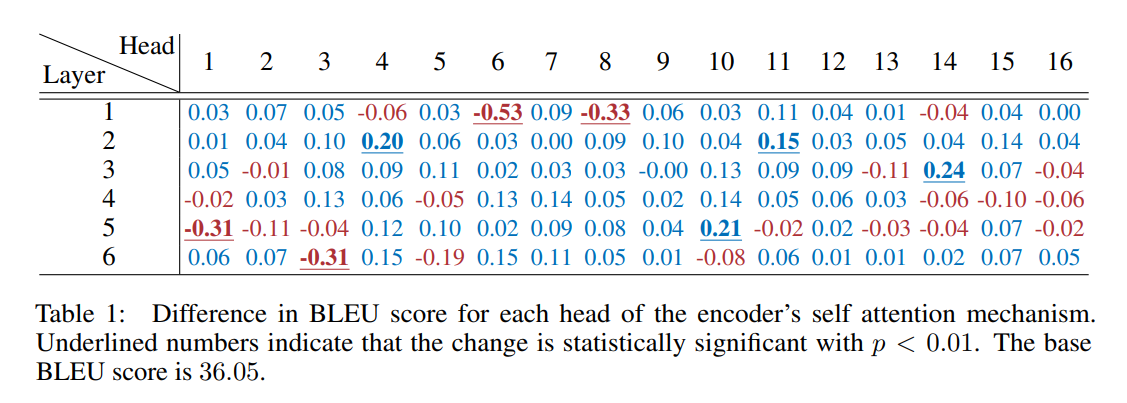
\includegraphics[width = 11cm]{figure/51-diffbleu.png}
	\end{figure}
		
	\begin{itemize}
		\item Only 8 (out of 96) heads cause a significant change in performance
		\item[] $\to$ \textbf{Observation:} At test time, most heads are redundant given the rest of the model.

	\end{itemize}
	
\vfill

\end{frame}

% ------------------------------------------------------------------------------

\begin{frame}{(2) inspecting different heads}

\vfill

\textbf{Are Sixteen Heads Really Better than One?} \citebutton{Michel et al., 2019}{https://papers.nips.cc/paper_files/paper/2019/hash/2c601ad9d2ff9bc8b282670cdd54f69f-Abstract.html}

	\begin{figure}
		\centering
		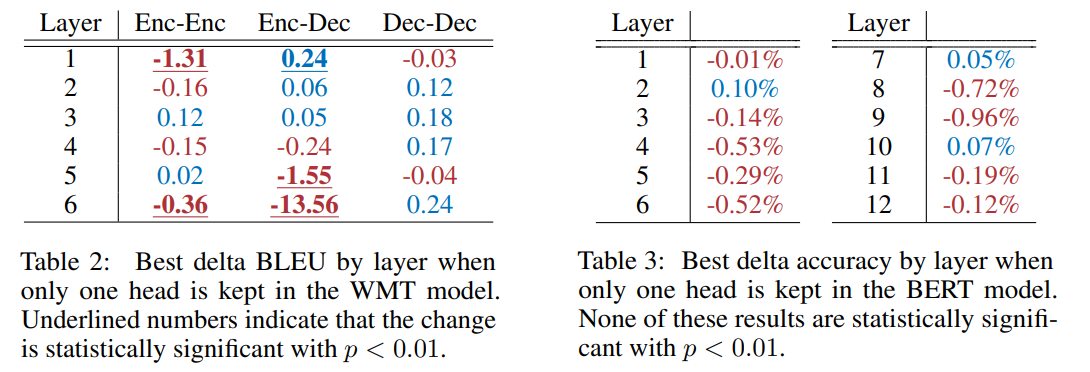
\includegraphics[width = 11cm]{figure/51-diffbleu-acc.png}
	\end{figure}
		
	\begin{itemize}
		\item For most layers, one head is indeed sufficient at test time
		\item However, some layers do require multiple attention heads\\
					(see Table 2, Enc-Dec attention in layer 6)
	\end{itemize}
	
\vfill

\end{frame}

% ------------------------------------------------------------------------------

\begin{frame}{(3) bertology summary}
\footnotesize% fit16:9


\vfill

\begin{itemize}
		\item \citebutton{Clark et al., 2019}{https://aclanthology.org/W19-4828/} and \citebutton{Michel et al., 2019}{https://papers.nips.cc/paper_files/paper/2019/hash/2c601ad9d2ff9bc8b282670cdd54f69f-Abstract.html} are just two prominent examples for widely recognized studies in this field of research
		\item Examining attention patterns/heads can yield insights into the model behaviour
		\item Huggingface example script for playing around: \citebutton{\texttt{bertology.py}}{https://github.com/huggingface/transformers/blob/main/examples/research_projects/bertology/run_bertology.py}
		\item \warning The research of \citebutton{Jain and Wallace, 2019}{https://aclanthology.org/N19-1357/} suggests that there is no direct connection between attention weights and other measures for explainability
		\item Many subsequent papers/models which aim at ..
			\begin{itemize}
				\item improving BERT \citebutton{RoBERTa (Liu et al., 2019)}{https://arxiv.org/abs/1907.11692} \citebutton{ALBERT (Lan et al., 2019)}{https://arxiv.org/abs/1909.11942}
				\item making BERT more efficient\\ \citebutton{ALBERT (Lan et al., 2019)}{https://arxiv.org/abs/1909.11942} \citebutton{DistilBERT (Sanh et al., 2019)}{https://arxiv.org/abs/1910.01108}
				\item modifying BERT \citebutton{BART (Lewis et al., 2019)}{https://arxiv.org/pdf/1910.13461.pdf} \citebutton{ELECTRA (Clark et al., 2020)}{https://arxiv.org/abs/2003.10555}
			\end{itemize}
		\item Overview on many different BERT-related papers:	\citebutton{BERT-related-papers}{https://github.com/tomohideshibata/BERT-related-papers}
\end{itemize}
\vfill

\end{frame}

% ------------------------------------------------------------------------------

\begin{frame}{(3) bertology summary}

\vfill

\textbf{Most architectures still rely on the transformer}

	\begin{figure}
		\centering
		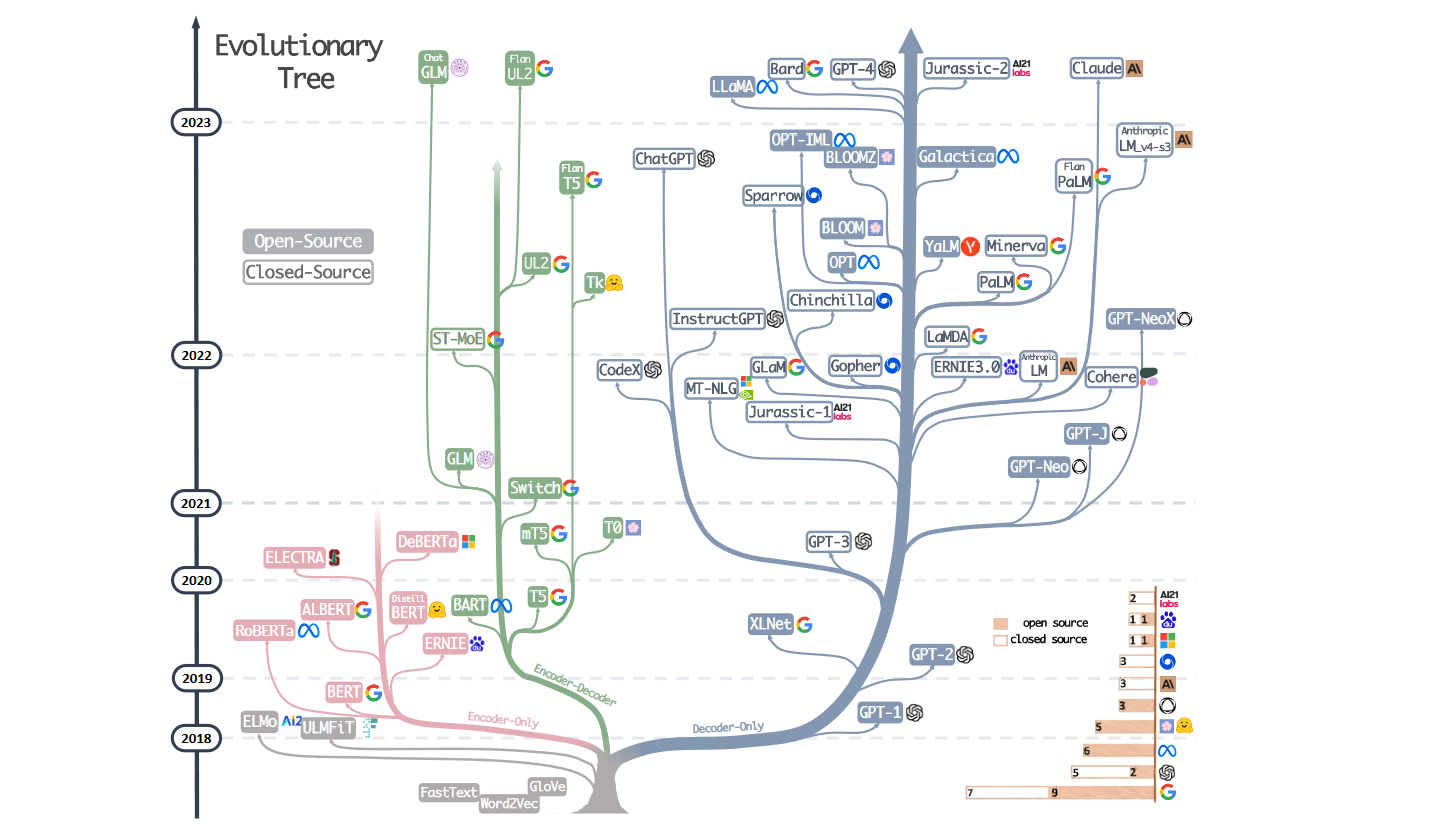
\includegraphics[width = 9.35cm]{figure/51-models.png}\\
		\citebutton{Source: Yang et al., 2023}{https://arxiv.org/abs/2304.13712}
	\end{figure}

\vfill

\end{frame}

% ------------------------------------------------------------------------------


%%%%%%%%%%%%%%%%%%%%%%%%%%%%%%%%%%%%%%%%%%%%%%%%%%%%%%%%%%%%%%%%%%
\section{BERT-based Architectures}
% Source: DL4NLP chapter05-bert-based/slides-52-bert-based.tex
%%%%%%%%%%%%%%%%%%%%%%%%%%%%%%%%%%%%%%%%%%%%%%%%%%%%%%%%%%%%%%%%%%
% ------------------------------------------------------------------------------

\begin{frame}{Sucessors of BERT}
\hbox{\hspace{-0.5em} 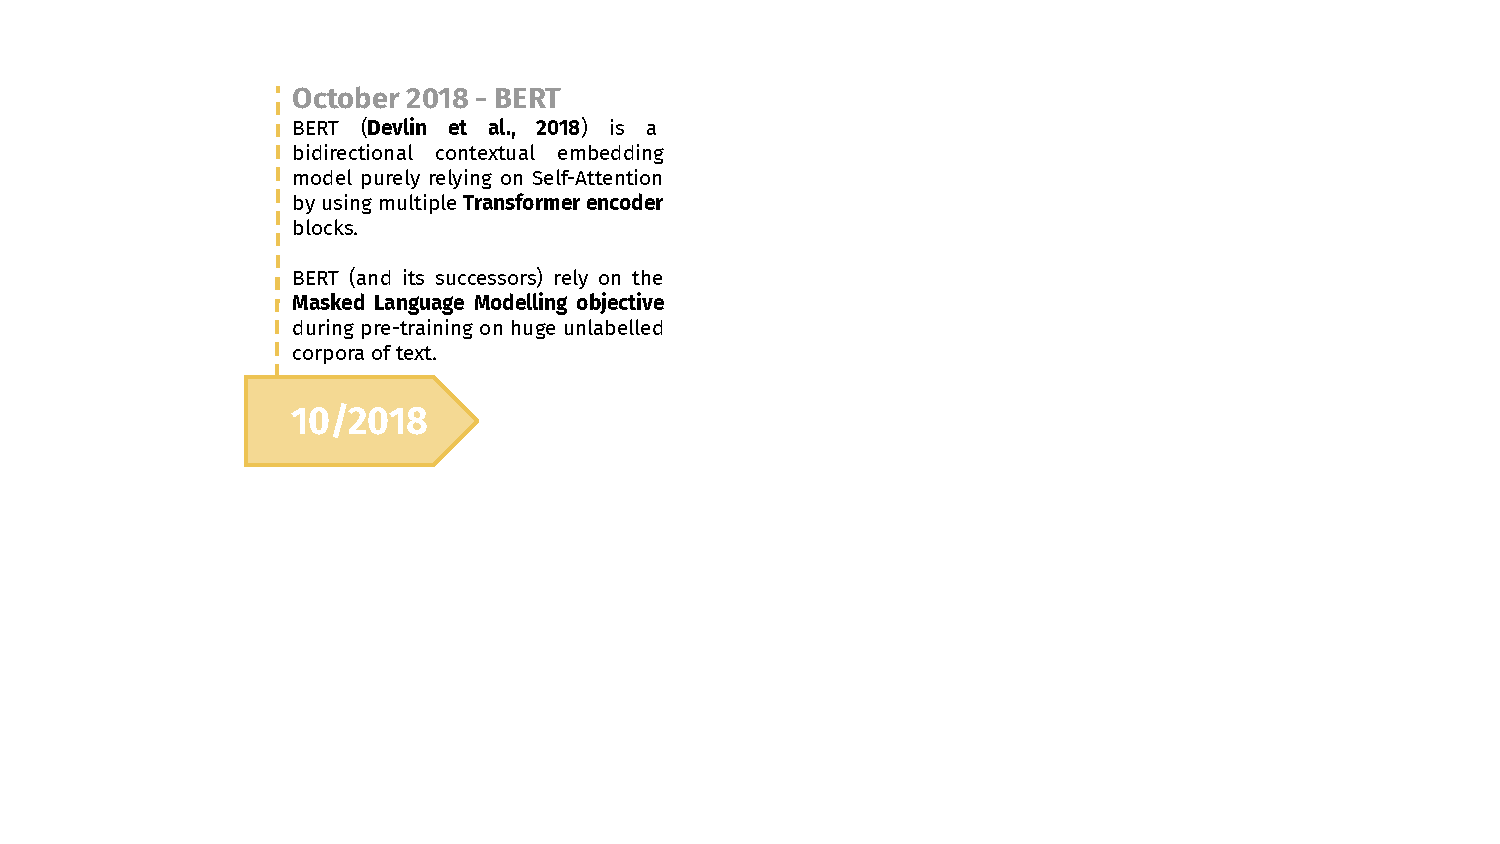
\includegraphics[width=12cm,page=1]{figure/transfer_learning_timeline3_nlp.pdf}}
\end{frame}
\begin{frame}[noframenumbering]{Sucessors of BERT}
\hbox{\hspace{-0.5em} \includegraphics[width=12cm,page=2]{figure/transfer_learning_timeline3_nlp.pdf}}
\end{frame}
\begin{frame}[noframenumbering]{Sucessors of BERT}
\hbox{\hspace{-0.5em} \includegraphics[width=12cm,page=3]{figure/transfer_learning_timeline3_nlp.pdf}}
\end{frame}
\begin{frame}[noframenumbering]{Sucessors of BERT}
\hbox{\hspace{-0.5em} \includegraphics[width=12cm,page=4]{figure/transfer_learning_timeline3_nlp.pdf}}
\end{frame}

% ------------------------------------------------------------------------------

\begin{frame}{roberta -- pre-training improvements}

\vfill

\textbf{R}obustly \textbf{o}ptimizied \textbf{BERT} \textbf{a}pproach \citebutton{Liu et al., 2019}{https://arxiv.org/abs/1907.11692}\\ \medskip\medskip

\textbf{Short summary:}

	\begin{itemize}
		\item Change of the \texttt{MASK}ing strategy  \\
					$\to$ BERT masks the sequences once before pre-training  \\
					$\to$ RoBERTa uses dynamic \texttt{MASK}ing  \\
					$\to$ RoBERTa sees the same sequence \texttt{MASK}ed differently
		\item RoBERTa \textbf{does not use} the additional NSP objective during pre-training
		\item Authors claim that BERT is seriously "undertrained"
			\begin{itemize}
				\item 160 GB pre-training corpus instead of 13 GB
				\item Pre-training is performed with larger batch sizes (8k)
			\end{itemize}
		\item Training on full-length sequences only (512 tokens)
	\end{itemize}
	
\vfill

\end{frame}

% ------------------------------------------------------------------------------
\begin{frame}{roberta -- the architecture}

\textbf{Architectural differences:}

\begin{itemize}
\item Architecture (layers, heads, embedding size) identical to BERT
\item 50k token BPE vocabulary instead of 30k
\item Model size differs (due to the larger embedding matrix)\\
			$\Rightarrow$ $\sim$ 125M (360M) for the BASE (LARGE) variant 
\end{itemize}

\textbf{Performance differences:}

\begin{figure}
\centering
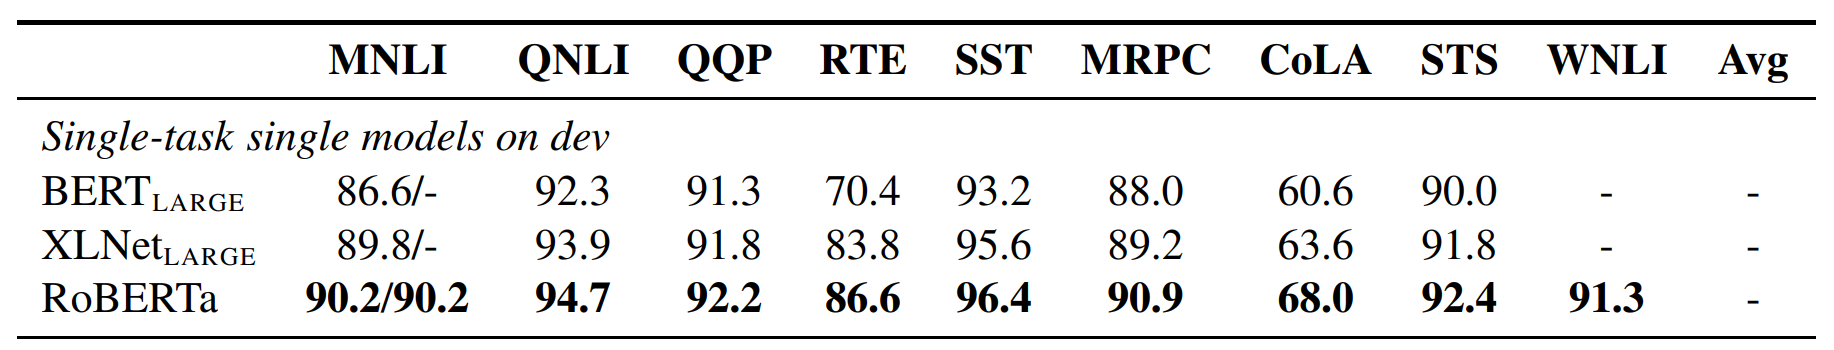
\includegraphics[width = 11cm]{figure/52-roberta-sota.png}\\ 
\citebutton{Source: Liu et al., 2019}{https://arxiv.org/abs/1907.11692}
\end{figure}

\vfill

\scriptsize
\textit{Note:} Liu et al. (2019) report the accuracy for QQP while Devlin et al. (2019) report the F1 score (cf. results displayed in chapter 6.2.3); XLNet: see next Chapter.

\end{frame}

% ------------------------------------------------------------------------------

\begin{frame}{Dynamic vs. Static Masking}

\vfill

	\textbf{Static Masking (BERT):}

	\begin{itemize}
		\item Apply \texttt{MASK}ing procedure to pre-training corpus once
		\item (additional for BERT: Modify the corpus for NSP)
		\item Train for approximately 40 epochs
	\end{itemize}

\vspace{.3cm}

	\textbf{Dynamic Masking (RoBERTa):}

	\begin{itemize}
		\item Duplicate the training corpus \textit{ten} times
		\item Apply \texttt{MASK}ing procedure to each duplicate of the pre-training corpus
		\item Train for 40 epochs
		\item Model sees each training instance in ten different "versions"\\
					(each version four times) during pre-training
	\end{itemize}
	
\vfill

\end{frame}

% ------------------------------------------------------------------------------

\begin{frame}{Dynamic vs. Static Masking}

\vfill

\begin{itemize}
	\item \normalsize \textbf{BERT:}
			\footnotesize
\begin{tabular}{|cccccccccc|}
\hline
The & quick & brown & \cellcolor{blue!65}\texttt{[MASK]} & jumps & over & the & \cellcolor{blue!65}\texttt{[MASK]} & dog & . \\
\hline
\end{tabular}
	\item[] \footnotesize
\begin{tabular}{|cccccccccc|}
\hline
The & quick & brown & \cellcolor{blue!65}\texttt{[MASK]} & jumps & over & the & \cellcolor{blue!65}\texttt{[MASK]} & dog & . \\
\hline
\end{tabular}
	\item[] \begin{center}$\vdots$\end{center}
	\item[] \footnotesize
\begin{tabular}{|cccccccccc|}
\hline
The & quick & brown & \cellcolor{blue!65}\texttt{[MASK]} & jumps & over & the & \cellcolor{blue!65}\texttt{[MASK]} & dog & . \\
\hline
\end{tabular}
\end{itemize}

\vspace{.75cm}

\begin{itemize}
	\item \normalsize \textbf{RoBERTa:}
			\footnotesize
\begin{tabular}{|cccccccccc|}
\hline
The & quick & brown & \cellcolor{blue!65}\texttt{[MASK]} & jumps & over & the & \cellcolor{blue!65}\texttt{[MASK]} & dog & . \\
\hline
\end{tabular}
	\item[] \footnotesize
\begin{tabular}{|cccccccccc|}
\hline
The & \cellcolor{blue!65}\texttt{[MASK]} & brown & fox & \cellcolor{blue!65}\texttt{[MASK]} & over & the & lazy & dog & . \\
\hline
\end{tabular}
	\item[] \footnotesize
\begin{tabular}{|cccccccccc|}
\hline
\cellcolor{blue!65}\texttt{[MASK]} & quick & \cellcolor{blue!65}\texttt{[MASK]} & fox & jumps & over & the & lazy & dog & . \\
\hline
\end{tabular}
	\item[] \begin{center}$\vdots$\end{center}
	\item[] \footnotesize
\begin{tabular}{|cccccccccc|}
\hline
\cellcolor{blue!65}\texttt{[MASK]} & quick & brown & fox & jumps & over & the & lazy & \cellcolor{blue!65}\texttt{[MASK]} & . \\
\hline
\end{tabular}
\end{itemize}

\vfill

\end{frame}

% ------------------------------------------------------------------------------

\begin{frame}{Dynamic vs. Static Masking}

\vfill

\begin{figure}
\centering
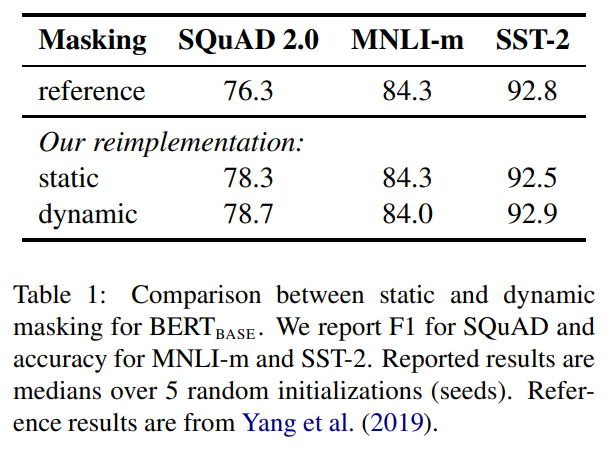
\includegraphics[width = 8cm]{figure/52-roberta-dynamic.png}\\ 
\citebutton{Source: Liu et al., 2019}{https://arxiv.org/abs/1907.11692}
\end{figure}

\vfill

\end{frame}

% ------------------------------------------------------------------------------

\begin{frame}{no next sentence prediction}

\vfill

	\begin{itemize}
		\item Described as important part of the pre-training process in BERT
		\item \citebutton{Liu et al., 2019}{https://arxiv.org/abs/1907.11692} report that it hurts performance
		\item[$\to$] Especially for QNLI, MNLI, and SQuAD 1.1
		\item Conduct experiments in multiple settings: 
			\begin{itemize}
				\item SEGMENT-PAIR+NSP
				\item[] \textit{(Exactly like BERT)}
				\item SENTENCE-PAIR+NSP
				\item[] \textit{(Like BERT, but with natural sentences)}
				\item FULL-SENTENCES
				\item[] \textit{(No NSP, inputs may cross document boundaries)}
				\item DOC-SENTENCES
				\item[] \textit{(No NSP, only sentences from one document)}
			\end{itemize}
	\end{itemize}
	
\vfill

\end{frame}

% ------------------------------------------------------------------------------
\begin{frame}{no next sentence prediction}

\vfill

\begin{figure}
\centering
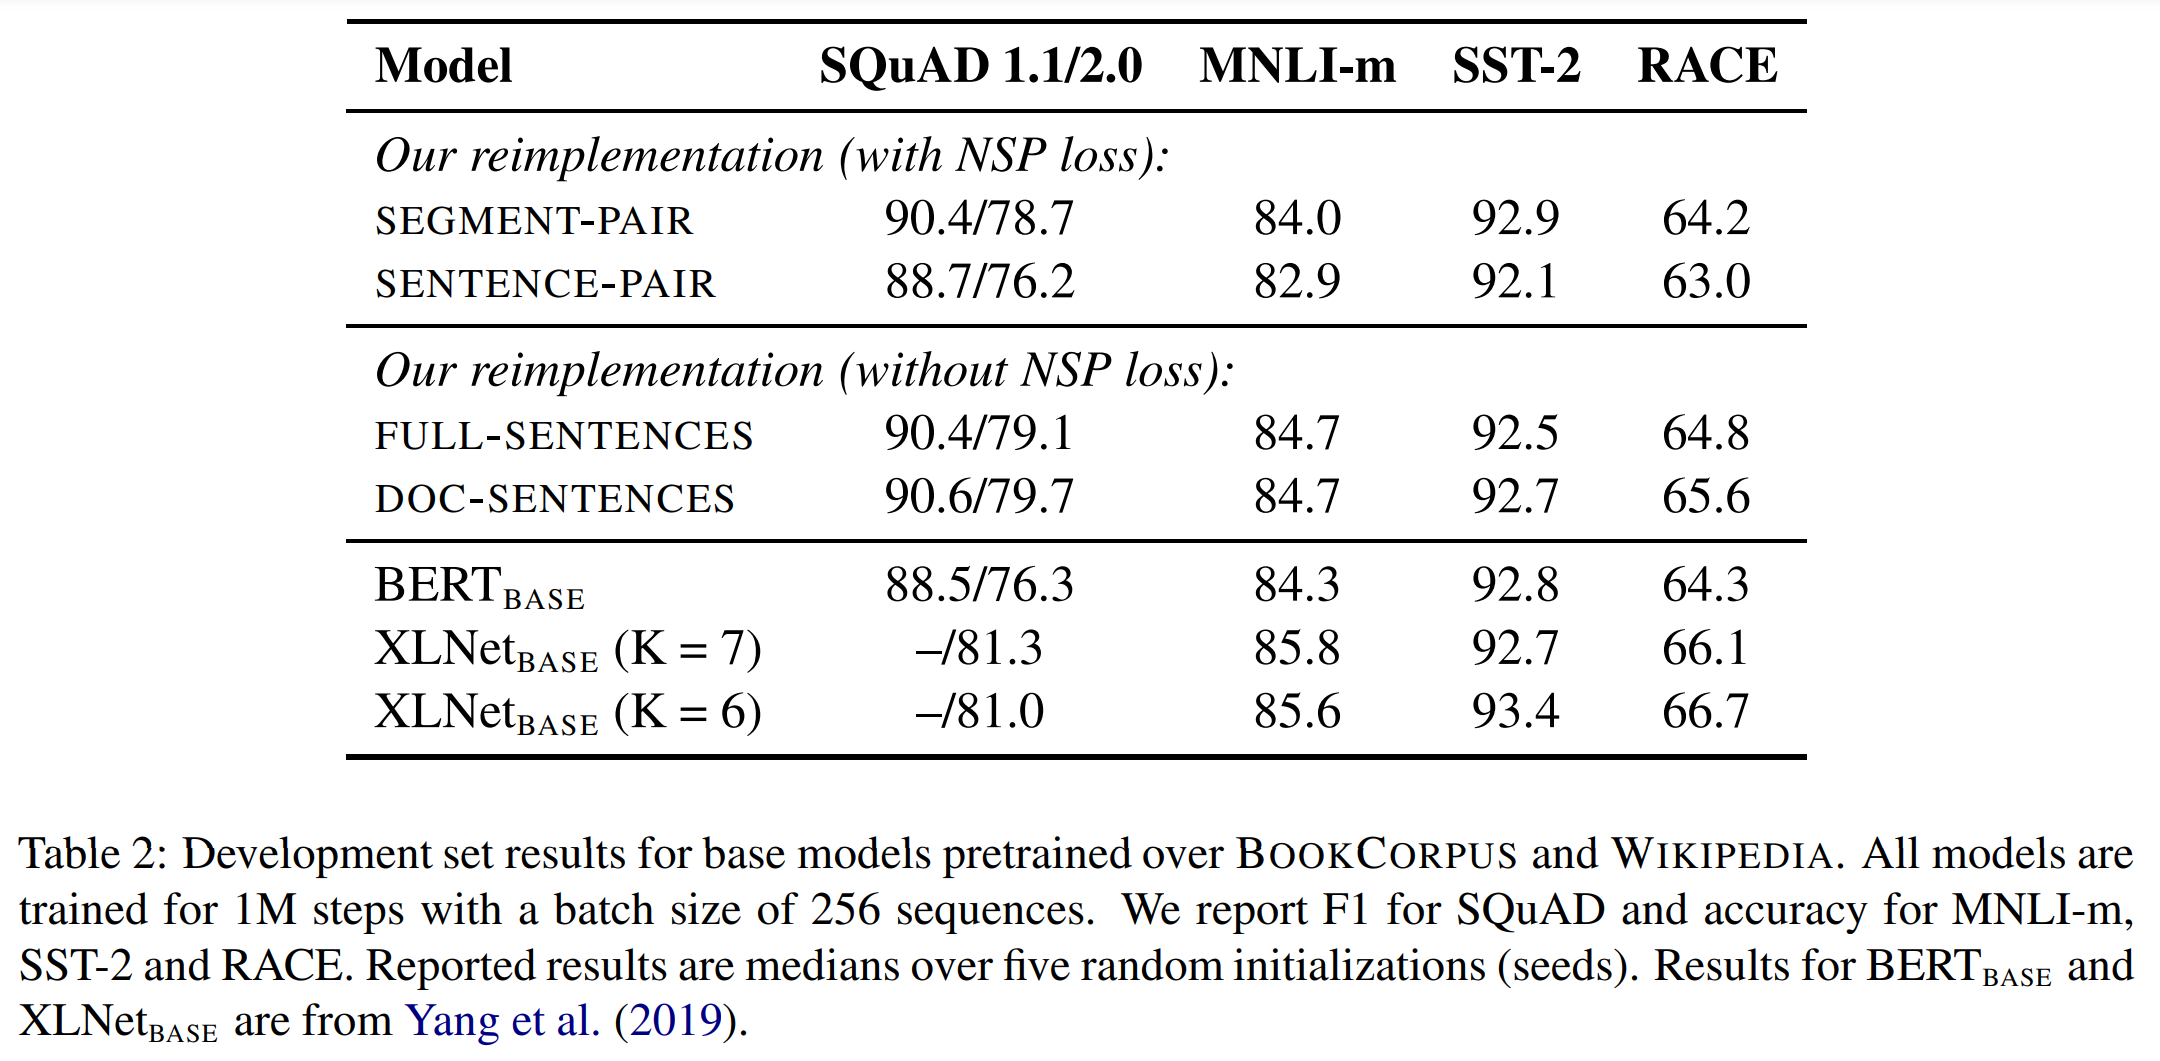
\includegraphics[width = 11cm]{figure/52-roberta-nsp.png}\\ 
\citebutton{Source: Liu et al., 2019}{https://arxiv.org/abs/1907.11692}
\end{figure}

\vfill

\scriptsize
\textit{Note:} XLNet: see next Chapter.

\end{frame}

% ------------------------------------------------------------------------------

\begin{frame}{batch size}

\vfill

\begin{figure}
\centering
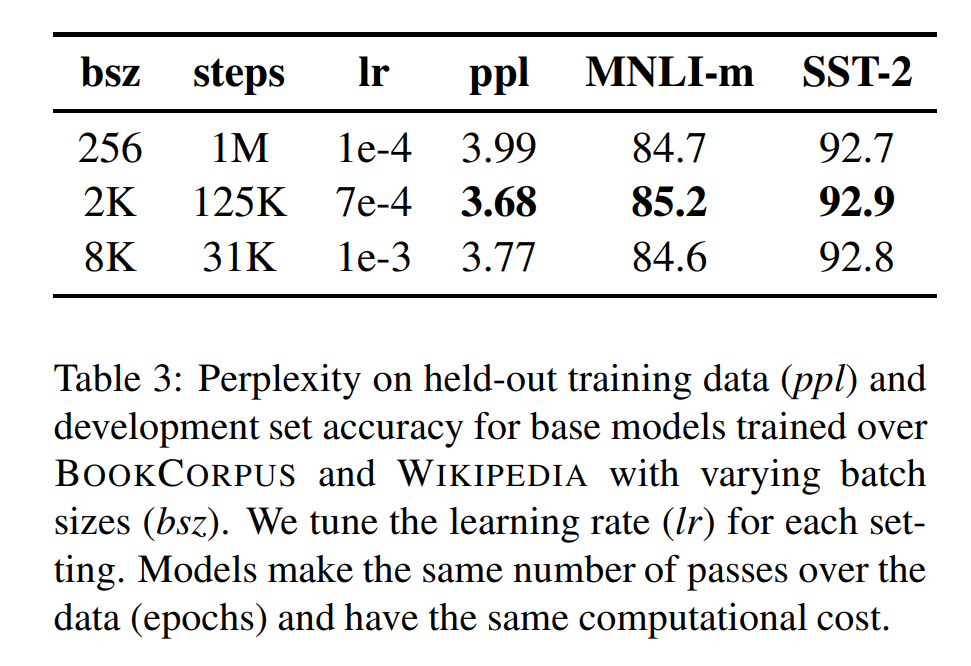
\includegraphics[width = 8cm]{figure/52-roberta-undertrained.png}\\ 
\citebutton{Source: Liu et al., 2019}{https://arxiv.org/abs/1907.11692}
\end{figure}

\vfill

\end{frame}

% ------------------------------------------------------------------------------

\begin{frame}{further changes in pre-training}

\vfill

\begin{figure}
\centering
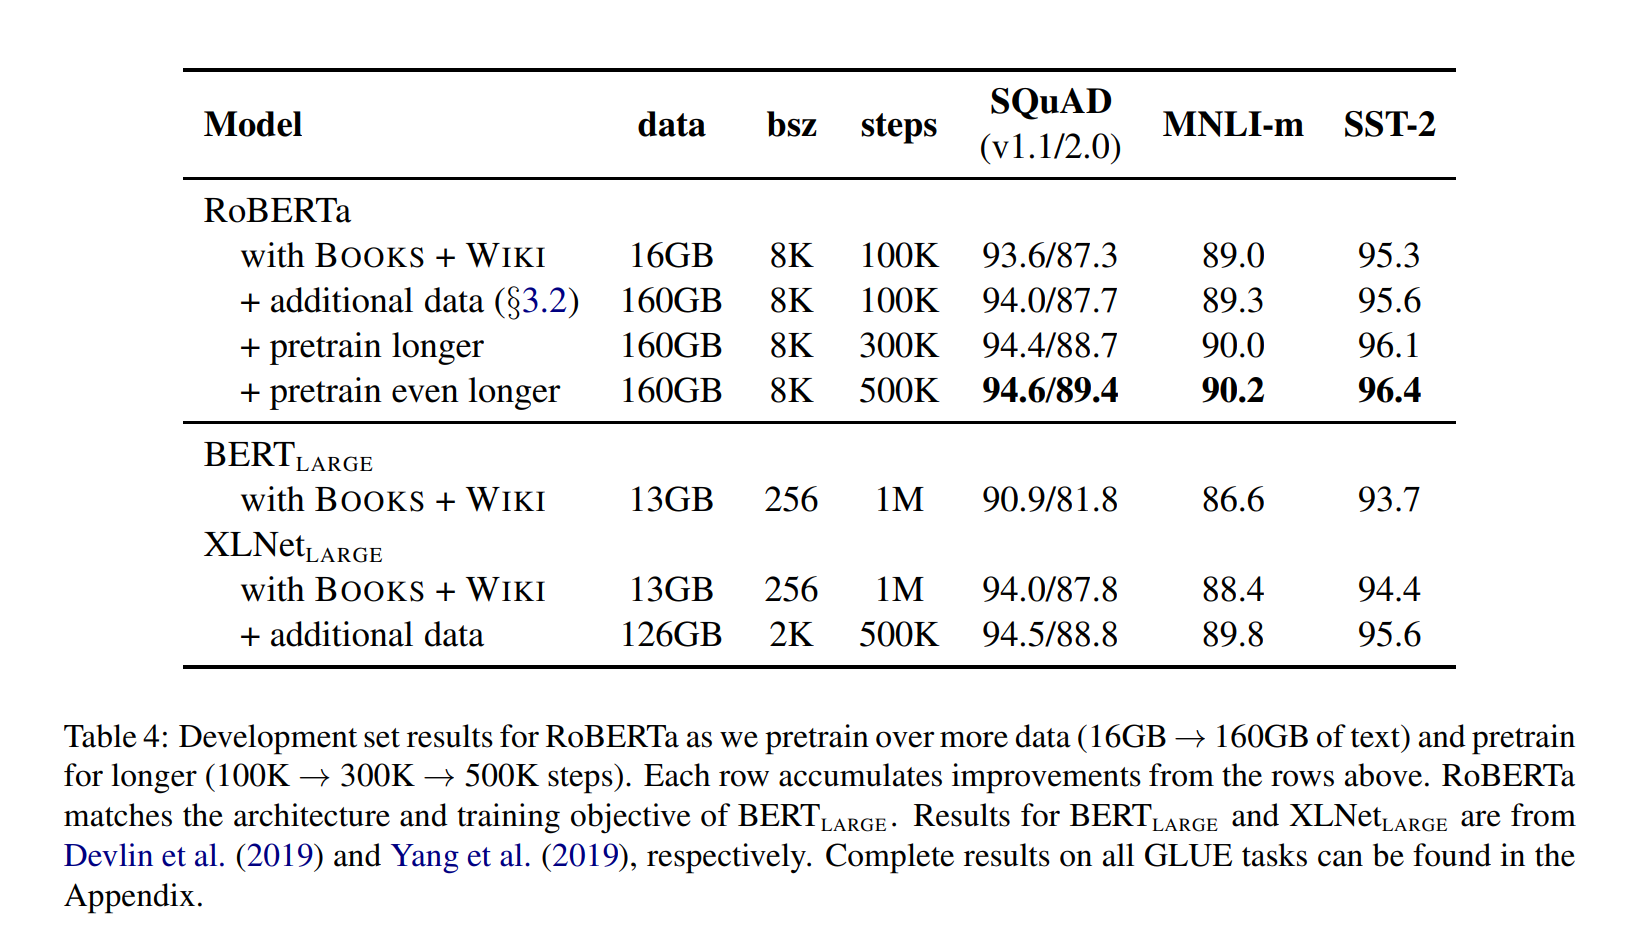
\includegraphics[width = 9.35cm]{figure/52-roberta-undertrained2.png}\\ 
\citebutton{Source: Liu et al., 2019}{https://arxiv.org/abs/1907.11692}
\end{figure}

\vfill

\scriptsize
\textit{Note:} XLNet: see next Chapter.

\end{frame}

% ------------------------------------------------------------------------------

\begin{frame}{albert}

\vfill

\textbf{A} \textbf{L}ite \textbf{BERT} \citebutton{Lan et al., 2019}{https://arxiv.org/abs/1909.11942}\\ \medskip\medskip

\textbf{Short summary:}

	\begin{itemize}
		\item Major change to the architecture \\
					$\to$ Size of embedding layer independent from hidden layer\\
					(rember in Transformer/BERT: $E = H$)\\
					$\to$ Saves memory and compute
		\item Parameter sharing across layers	
		\item Substitution of the NSP objective during pre-training
	\end{itemize}
	
\vfill

\end{frame}

% ------------------------------------------------------------------------------
\begin{frame}{architectural changes}

\vfill

	\textbf{Disentanglement of $E$ and $H$}

	\begin{itemize}
		\item	WordPiece-Embeddings (size $E$) 
			\begin{itemize}
				\item first layer of the model
				\item each token is initially mapped to this embedding
				\item context-independent
			\end{itemize}
		\item In Transformer/BERT: 
			\begin{itemize}
				\item $H = E$
				\item down-project $E$ to keys, queries and values of size $H/A$
				\item concatenate resulting embeddings from all $A$ heads
				\item results in hidden layer representation of size $H$
			\end{itemize}
		\item \ques What are the implications?
	\end{itemize}

\vfill

\end{frame}

% ------------------------------------------------------------------------------

\begin{frame}{architectural changes}

\vfill

\textbf{Thoughts / Implications}

	\begin{itemize}
		\item	WordPiece-Embeddings (size $E$) 
			\begin{itemize}
				\item required representational capacity?
				\item probably could be limited w/o loosing much
			\end{itemize}
		\item Hidden-Layer-Embedding (size $H$)
			\begin{itemize}
				\item required representational capacity?
				\item depending on how polysemous a word/token might be
				\item difficult to say "one size fits all"
				\item probably might be better to rather increase this, compared to the WordPiece embeddings
			\end{itemize}
	\end{itemize}
	
\vspace{.5cm}

$\to$ \textit{Setting $E = H$ does not allow us to pursue these considerations}

\vfill

\end{frame}

% ------------------------------------------------------------------------------

\begin{frame}{architectural changes}

\vfill

\textbf{Disentanglement solves this}

	\begin{itemize}
		\item Hidden-Layer-Embeddings (size $H$) context-dependent\\
					$\to$ providing more capacity makes more sense here
		\item Setting $H >> E$ enlargens model capacity in the hidden layers without increasing the size of the embedding matrix
		\item $O(V \times H) > O(V \times E +  E \times H)$ if $H >> E$
\end{itemize}

\vfill

\end{frame}

% ------------------------------------------------------------------------------

\begin{frame}{Cross-Layer parameter sharing}

\vfill

	\begin{itemize}
		\item Pre-trained transformer-based models are deep stacks of identically parametrized layers and thus have many parameters
		\item Sharing them as a way to gain parameter efficiency
		\item Two different places in the network, where sharing can be done
			\begin{itemize}
				\item Attention parameters
				\item FFN parameters
			\end{itemize}
		\item Ablation studies: 
			\begin{itemize}
				\item both
				\item both individually
				\item none
			\end{itemize}
	\end{itemize}

\vfill

\end{frame}

% ------------------------------------------------------------------------------

\begin{frame}{Cross-Layer parameter sharing}

\vfill

	\begin{figure}
		\centering
		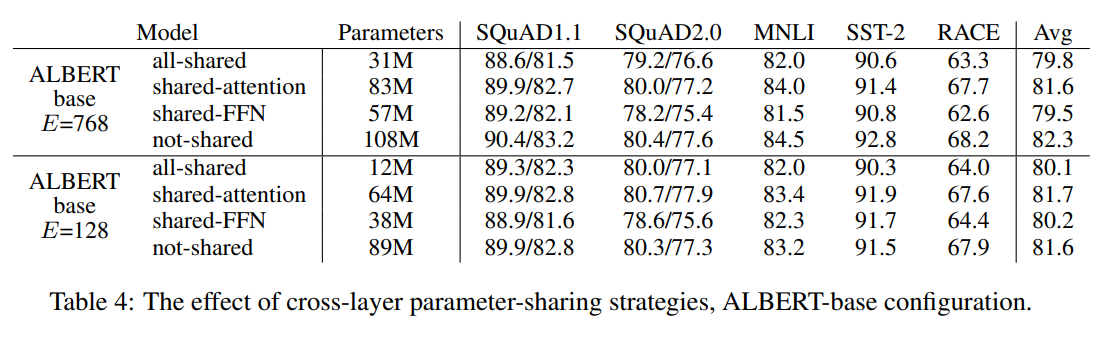
\includegraphics[width = 11cm]{figure/52-albert-param-sharing.png}\\ 
		\citebutton{Source: Lan et al., 2019}{https://arxiv.org/pdf/1909.11942.pdf}
	\end{figure}

	\begin{itemize}
		\item (Drastic) reduction of model size (more for sharing FFN weights)
		\item Sharing parameters hurts performance
			\begin{itemize}
				\item Worse for models with larger $E$
				\item Worse for sharing FNN compared to Attention weights
		\item \ques \textbf{Why? What is the intuition here?}
			\end{itemize}
	\end{itemize}


\vfill

\end{frame}

% ------------------------------------------------------------------------------

\begin{frame}{Cross-Layer parameter sharing}

\vfill

	\begin{figure}
		\centering
		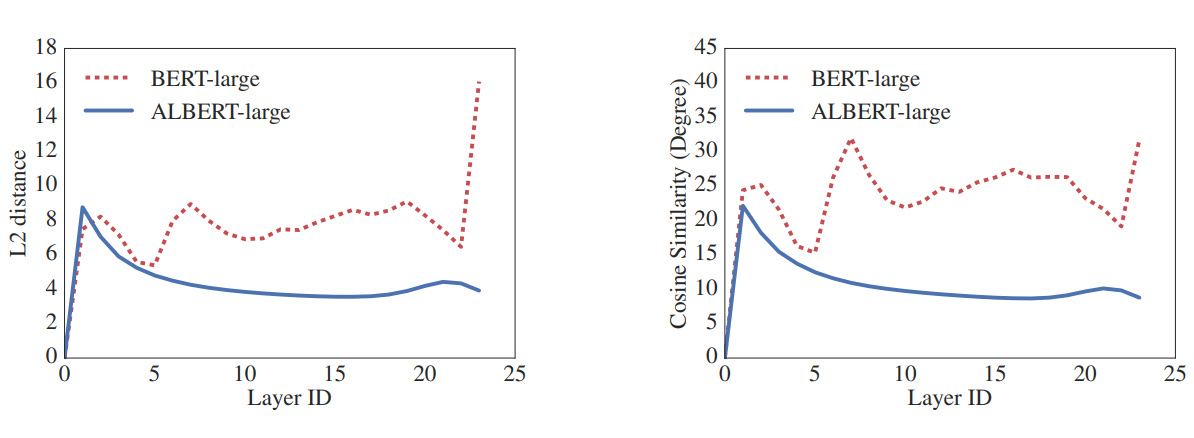
\includegraphics[width = 11cm]{figure/52-albert-param-sharing2.png}\\ 
		\citebutton{Source: Lan et al., 2019}{https://arxiv.org/pdf/1909.11942.pdf}
	\end{figure}
	
\begin{itemize}
	\item Distince/Similarity of input and output embeddings per layer
	\item Smoother transitions for ALBERT models
\end{itemize}

\vfill

\end{frame}

% ------------------------------------------------------------------------------

\begin{frame}{Changes in pre-training}

\vfill

	\textbf{Substitution of the NSP objective}
		
	\begin{itemize}
			\item Previous works questioned the usefulness of NSP
			\item[$\to$] Lan et al. assume that this is due to lacking difficulty
			\item Introduction of \textit{Sentence-Order Prediction} (SOP) as a new pre-training task
			\item Positive examples created alike to those from NSP (take two consecutive sentences from the same document)
			\item Negative examples: Just swap the ordering of sentences
	\end{itemize}

\vfill

\end{frame}

% ------------------------------------------------------------------------------

\begin{frame}{Changes in pre-training}

\vfill

	\textbf{Illustration:}
		
	\begin{figure}
		\centering
		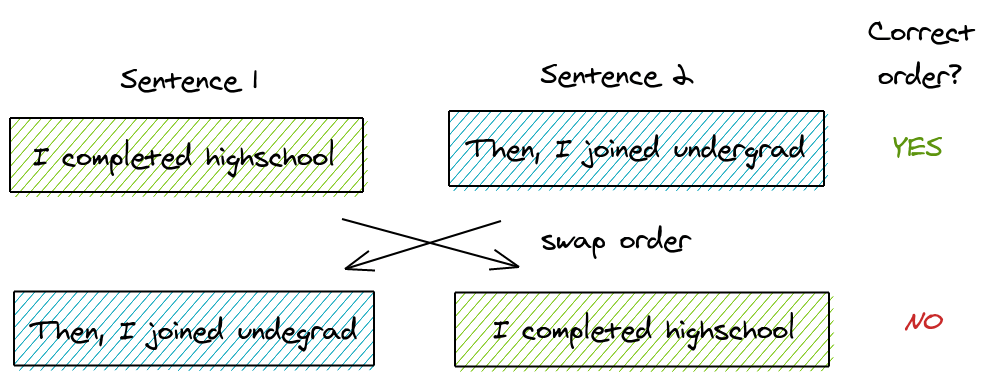
\includegraphics[width = 6.80cm]{figure/52-albert-sop.png}\\ 
		\citebutton{Source: Amit Chaudhary}{https://amitness.com/2020/02/albert-visual-summary/}
	\end{figure}

	\textbf{Effectiveness:}
		
	\begin{figure}
		\centering
		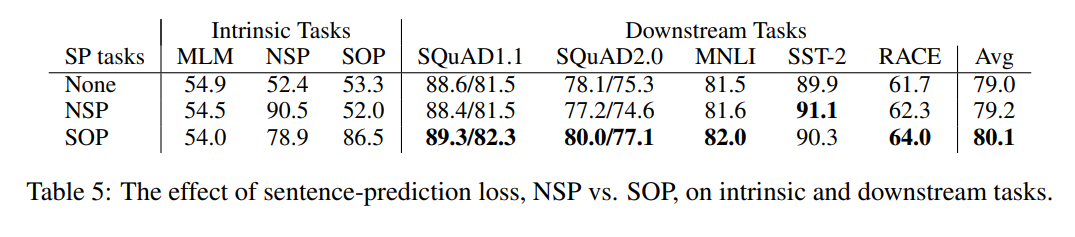
\includegraphics[width = 8.50cm]{figure/52-albert-sop-ablation.png}\\ 
		\citebutton{Source: Lan et al., 2019}{https://arxiv.org/pdf/1909.11942.pdf}
	\end{figure}

\vfill

\end{frame}

% ------------------------------------------------------------------------------

\begin{frame}{Changes in pre-training}

\vfill

	\textbf{$n-gram$ masking for the MLM task}
		
	\begin{itemize}
			\item During pre-training BERT single tokens are masked
			\item Lan et al. mask up to three consecutive tokens
			\item Choice of $n$:\\
						\begin{center}
							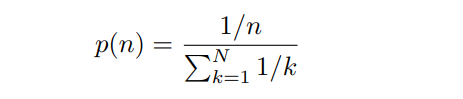
\includegraphics[width = 6cm]{figure/52-albert-choice-n.png}
						\end{center}
	\end{itemize}

\vfill

\end{frame}

% ------------------------------------------------------------------------------

\begin{frame}{performance}

	\textbf{Performance differences:}

	\begin{figure}
		\centering
		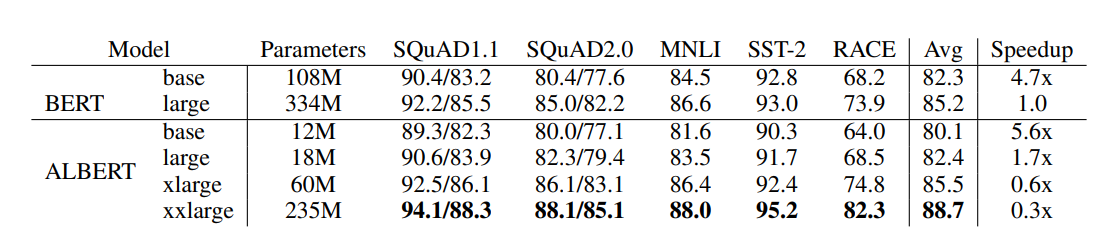
\includegraphics[width = 11cm]{figure/52-albert-sota.png}\\ 
		\citebutton{Source: Lan et al., 2019}{https://arxiv.org/pdf/1909.11942.pdf}
	\end{figure}

	\textbf{Notes:}

	\begin{itemize}
		\item In General: Smaller model size (because of parameter sharing)
		\item Nevertheless: Scale model up to almost similar size\\(\texttt{xxlarge} version)
		\item Strong performance compared to BERT
	\end{itemize}
\end{frame}

% ------------------------------------------------------------------------------


%%%%%%%%%%%%%%%%%%%%%%%%%%%%%%%%%%%%%%%%%%%%%%%%%%%%%%%%%%%%%%%%%%
\section{Model Distillation}
% Source: DL4NLP chapter05-bert-based/slides-53-distilbert.tex
%%%%%%%%%%%%%%%%%%%%%%%%%%%%%%%%%%%%%%%%%%%%%%%%%%%%%%%%%%%%%%%%%%
% ------------------------------------------------------------------------------

\begin{frame}{model compression}

\vfill

\textbf{Motivation:} \citebutton{Bucila et al., 2006}{http://www.niculescu-mizil.org/papers/rtpp364-bucila.rev2.pdf}

\begin{itemize}
				\item Existence of computationally expensive, cumbersome ensemble models
				\item Accuracy/Performance not everything that should be taken into account (also interpretability and deployability)
				\item Time and space requirements also of importance
				\item \textit{Model Compression} aims ``to obtain fast, compact yet highly accurate models``
				\item The fast and compact model should approximate the function learned by the slower and larger model
\end{itemize}

\vfill

\end{frame}

% ------------------------------------------------------------------------------

\begin{frame}{Model compression}

\vfill

\textbf{Advantages:}

\begin{itemize}
	\item Compressing the knowlegde of the ensemble into a single model has the benefits of
			\begin{itemize}
				\item easier deployment
				\item better generalization
				\item (potential) interpretability
			\end{itemize} 
	\item \textit{Reasoning:}
		\begin{itemize}
			\item Cumbersome model generalizes well, because it is the average of an ensemble
			\item Small model trained to generalize in the same way typically better than small model trained "the normal way"
		\end{itemize}
\end{itemize}

\vfill

\end{frame}

% ------------------------------------------------------------------------------

\begin{frame}{Model compression}

\vfill

\begin{itemize}
	\item \textit{Challenge}: 
			\begin{itemize}
				\item Bucila et al. assumed only knowledge about the weights of the large (ensemble) model
				\item No access to its training data
				\item[] $\to$ Their work is mainly on generating suitable pseudo data for model compression
			\end{itemize} 
	\item \textit{NLP:}
		\begin{itemize}
			\item Abundant amounts of data; no need for creating pseudo data
			\item Self-supervised objectives can be used for model compression
		\end{itemize}
\end{itemize}

\vfill

\end{frame}

% ------------------------------------------------------------------------------

\begin{frame}{Model distillation}

\textbf{Motivation:}
	\begin{figure}
		\centering
		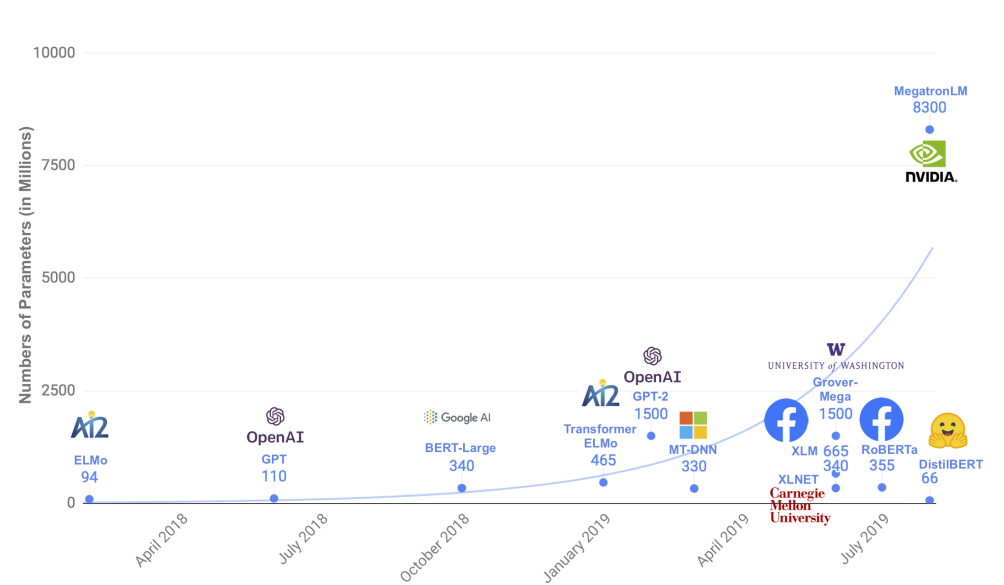
\includegraphics[width = 10cm]{figure/53-distilbert-motivation}\\ 
		\citebutton{Source: Sanh et al., 2019}{https://arxiv.org/pdf/1910.01108.pdf}
	\end{figure}
	
\end{frame}

% ------------------------------------------------------------------------------

\begin{frame}{Model distillation}

\vfill

\textbf{Types of targets} 

\begin{itemize}
	\item ``\textit{Hard}`` Targets $$[0, 0, 0, 1, 0]$$ \vspace{-.5cm}
		\begin{itemize}
			\item Present when learning from labeled data
			\item Ordinary way of training models
		\end{itemize}
	\item Knowledge transfer possible via ``\textit{soft}`` targets from original model
	\item Possible ``\textit{soft}`` targets
		\begin{itemize}
			\item Logits + L2 loss \citebutton{Bucila et al., 2006}{http://www.niculescu-mizil.org/papers/rtpp364-bucila.rev2.pdf}
			\item Softmax scores
			\item Temperature $T$ in the softmax \citebutton{Hinton et al., 2015}{https://arxiv.org/abs/1503.02531}
						$$q_i = \frac{\exp(z_i/T)}{\sum_j \exp(z_j/T)}$$
		\end{itemize}
\end{itemize}

\vfill

\end{frame}

% ------------------------------------------------------------------------------

\begin{frame}{Model distillation}

\vfill

\textbf{Temperature:}\\$$q_i = \frac{\exp(z_i/T)}{\sum_j \exp(z_j/T)}$$

\begin{itemize}
	\item \textit{Why?} Produce a softer probability distribution over classes
	\item $z_i$/$z_j$ are the raw logits
	\item Parameter $T$ controls to smoothness of the distribution
		\begin{itemize}
			\item Higher $T$: ``softer`` distribution
			\item Lower $T$: more pronounced distribution
		\end{itemize}
	\item \textit{Distillation phase}: Apply same temperature to teacher and student
	\item \textit{Inference}: Set $T = 1$ to recover standard softmax						
\end{itemize}

\vfill

\end{frame}

% ------------------------------------------------------------------------------

\begin{frame}{Model distillation}

\vfill

\textbf{Intuition}

\begin{itemize}
	\item Train the student to \textit{mimick} the teacher's behaviour
	\item \ques Advantage of the soft targets:
	\item[] $\to$ No need to know the true labels of the training instances
	\item[] $\to$ More fine-grained information about the teacher's behaviour 
	\item When true labels are known:\\
				Weighted average of two different objective functions possible\\
	\item[] $\to$ On soft targets (\textit{Be close to the teacher}) and 
	\item[] $\to$ on hard targets (\textit{be close to the ``ground truth``})
\end{itemize}

\vfill

\end{frame}

% ------------------------------------------------------------------------------

\begin{frame}{distilbert}

\vfill

\textbf{Characteristics of the student architecture:}

\begin{itemize}
	\item Half the number of layers compared to BERT$^1$ (6 instead of 12)
	\item Remove segment embeddings$^2$ (required for NSP objective)
 	\item Half of the size of BERT, but retains up to 97\% of the performance on GLUE
	\item Initialize from BERT (taking one out of two hidden layers)
	\item Same pre-training data as BERT (Wiki + BooksCorpus)
\end{itemize}

\vfill

{\footnotesize $^1$Rationale for "only" reducing the number of layers:\\
Larger influence on the computation efficiency compared to e.g. hidden size dimension\\
$^2$ Sanh et al. call them ``token-type embeddings`` in their paper}

\end{frame}

% ------------------------------------------------------------------------------

\begin{frame}{distilbert}

\vfill

\textbf{Combination of three different loss functions:}

\begin{itemize}
	\item \textit{Soft targets:}\\Distillation loss $L_{ce} = \sum_i t_i \cdot \log(s_i)$
	\item \textit{Hard targets:}\\Masked language modeling loss $L_{mlm}$ (cf. BERT)
	\item \textit{Alignment:}\\Cosine-Embedding-Loss $L_{cos} = 1 - \frac{\vec w^{(i)T}\vec w^{(j)}}{\lVert \vec w^{(i)} \rVert_2 \cdot \lVert \vec w^{(j)}\lVert_2}$\\
				(\textit{Rationale:} Keep DistilBERT's embeddings close to BERT's)
\end{itemize}

\vspace{.3cm}

\textbf{Adopt improvement from RoBERTa:}

\begin{itemize}
	\item Stop using the NSP loss (hence removed segment embeddings)
	\item Dynamic masking for MLM
	\item Train with large batches
\end{itemize}

\vfill

\end{frame}

% ------------------------------------------------------------------------------

\begin{frame}{distilbert}

\vfill

	\textbf{Performance differences to BERT:}

	\begin{figure}
		\centering
		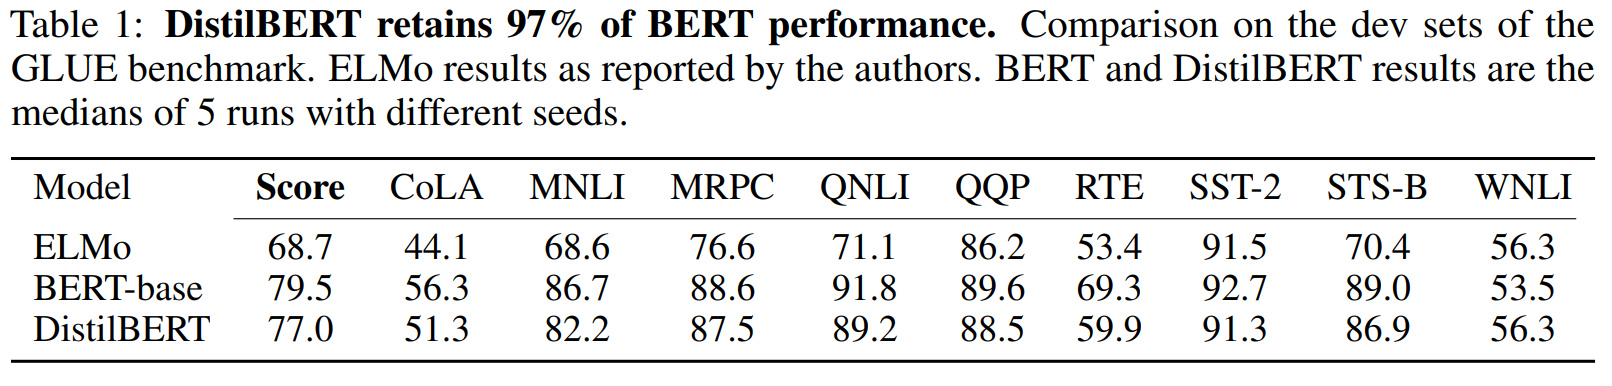
\includegraphics[width = 11cm]{figure/53-distilbert-vs-sota.png}\\ 
		\citebutton{Source: Sanh et al., 2019}{https://arxiv.org/pdf/1910.01108.pdf}
	\end{figure}


\textbf{Takeaways:}

\begin{itemize}
	\item Largest performance on textual entailment task (RTE)
	\item Even better reported performance on Winograd schemas (WNLI)
	\item \textit{Overall:} Very consistent performance a little worse than BERT
\end{itemize}

\vfill

\end{frame}

% ------------------------------------------------------------------------------

\begin{frame}{distilbert}

\vfill

	\textbf{Ablation study regarding the loss:}

	\begin{figure}
		\centering
		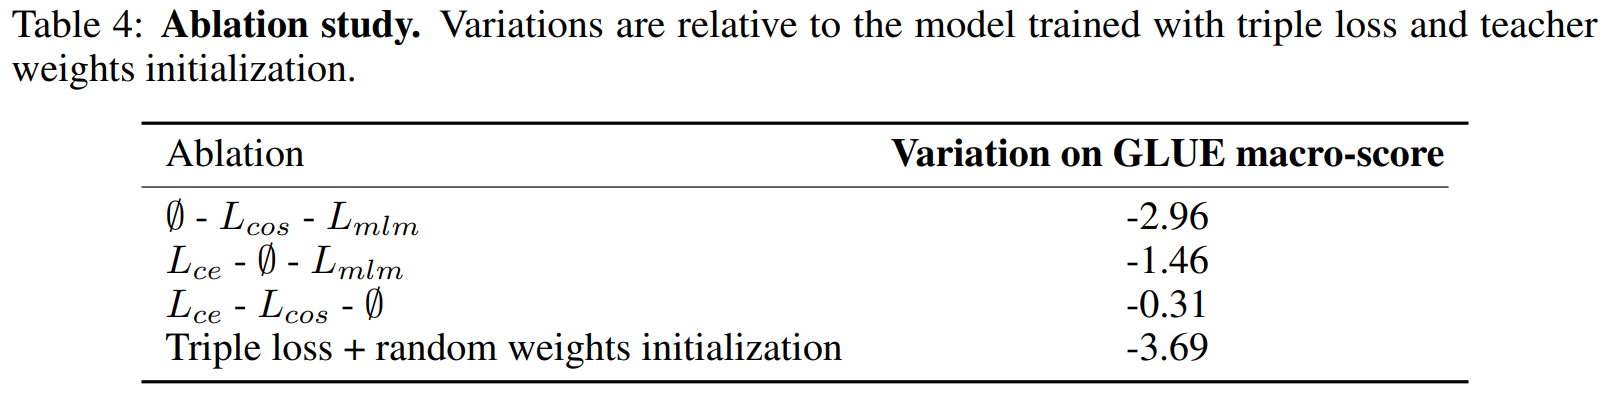
\includegraphics[width = 11cm]{figure/53-distilbert-ablation.png}\\ 
		\citebutton{Source: Sanh et al., 2019}{https://arxiv.org/pdf/1910.01108.pdf}
	\end{figure}

\textbf{Takeaways:}

\begin{itemize}
	\item Start training from BERT's weights is crucial
	\item Removing MLM loss has little impact\\
	\item[] $\to$ Signal in the soft targets sufficiently strong
	\item Notable contribution of the cosine embedding loss
\end{itemize}

\vfill
	
\end{frame}

% ------------------------------------------------------------------------------

\begin{frame}{distilbert}

\vfill

\textbf{Size and speed:}

	\begin{figure}
		\centering
		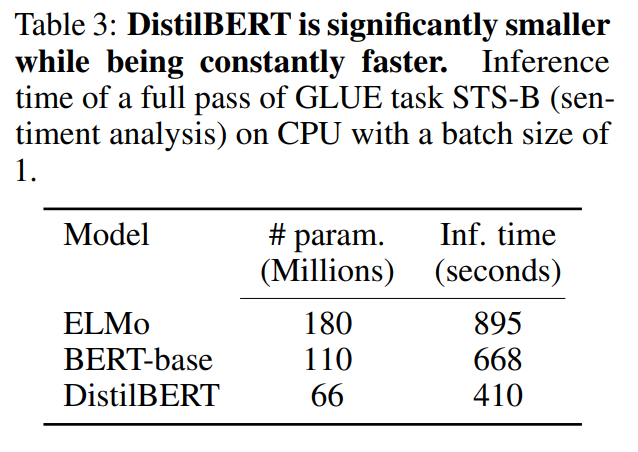
\includegraphics[width = 6.5cm]{figure/53-distilbert-size-speed.png}\\ 
		\citebutton{Source: Sanh et al., 2019}{https://arxiv.org/pdf/1910.01108.pdf}
	\end{figure}

\vfill
	
\end{frame}

% ------------------------------------------------------------------------------

\begin{frame}{related approaches (1)}

\vfill

\textbf{Quantization:}

\begin{itemize}
	\item \textit{In General:} Mathematical procedure of converting a number from a continuous scale to a discrete scale
	\item \textit{In Machine Learning (usually):} Convert a number from high precision (float16/float32) to a lower precision (float8/int8) 
	\item For models with billions of parameters, this can save enormous amount of memory
	\item Given that model sizes (at the moment) grow faster than GPU memory, this can be crucial for even making \textit{inference} of large models feasible
	\item \textit{Trade-Off:} Memory savings vs. model quality
\end{itemize}

\vfill
	
\end{frame}

% ------------------------------------------------------------------------------

\begin{frame}{related approaches (2)}

\vfill

\textbf{Pruning:}

\begin{itemize}
	\item Remove (``\textit{prune}``) certain parts of the model according to some score measuring the importance of that part for performance 
	\item Common importance score (in NLP):\\Sensitivity of the loss wrt the values of the neurons \citebutton{Yang et al., 2022}{https://arxiv.org/abs/2203.15996}
							$$\mathrm{IS}(\bm\Theta) = \mathbb{E}_{x\sim X}\left\lvert \frac{\partial \mathcal{L}(x)}{\partial\bm\Theta}\bm\Theta \right\rvert$$
	\item Common choices for $\bm\Theta$ (in Transformers):
			\begin{itemize}
				\item Output of an attention head
				\item An intermediate neuron in the FFN layer
			\end{itemize}
\end{itemize}

\vfill
	
\end{frame}

% ------------------------------------------------------------------------------

\begin{frame}{related approaches (2)}

\vfill

\textbf{Self-supervised Pruning} \citebutton{Yang et al., 2022}{https://arxiv.org/abs/2203.15996}

\begin{itemize}
	\item Substitute $\mathcal{L}$ by
							$$\mathcal{L}_{\mathrm{KL}}(x)=\mathrm{KL}(\mathrm{stopgrad}(q(x))||p(x)),$$
	\item where
			\begin{itemize}
				\item $q(x)$ is the original model prediction distribution,
				\item $p(x)$ is the to-be-pruned model prediction distribution,
				\item and \texttt{stopgrad} is used to stop back-propagating gradients
			\end{itemize}
\end{itemize}

\vfill
	
\end{frame}

% ------------------------------------------------------------------------------

\begin{frame}{summary}

\vfill

\begin{itemize}
	\item Model compression/distillation against growing model sizes
	\item DistilBERT as a powerful, small alternative to BERT
	\item Other approaches (pruning) that allow for a more targeted ``deactivation`` of individual heads (and might thus also improve interpretability)
	\item Quantization as an approach to \textit{significantly} reduce the memory requirements of large models
\end{itemize}

\vfill
	
\end{frame}

% ------------------------------------------------------------------------------


%%%%%%%%%%%%%%%%%%%%%%%%%%%%%%%%%%%%%%%%%%%%%%%%%%%%%%%%%%%%%%%%%%
\section{Post-BERT Architectures}
% Source: DL4NLP chapter06-post-bert-t5/slides-61-postbert.tex
%%%%%%%%%%%%%%%%%%%%%%%%%%%%%%%%%%%%%%%%%%%%%%%%%%%%%%%%%%%%%%%%%%
% ------------------------------------------------------------------------------

\begin{frame}{Successors of BERT}
\hbox{\hspace{-3em} 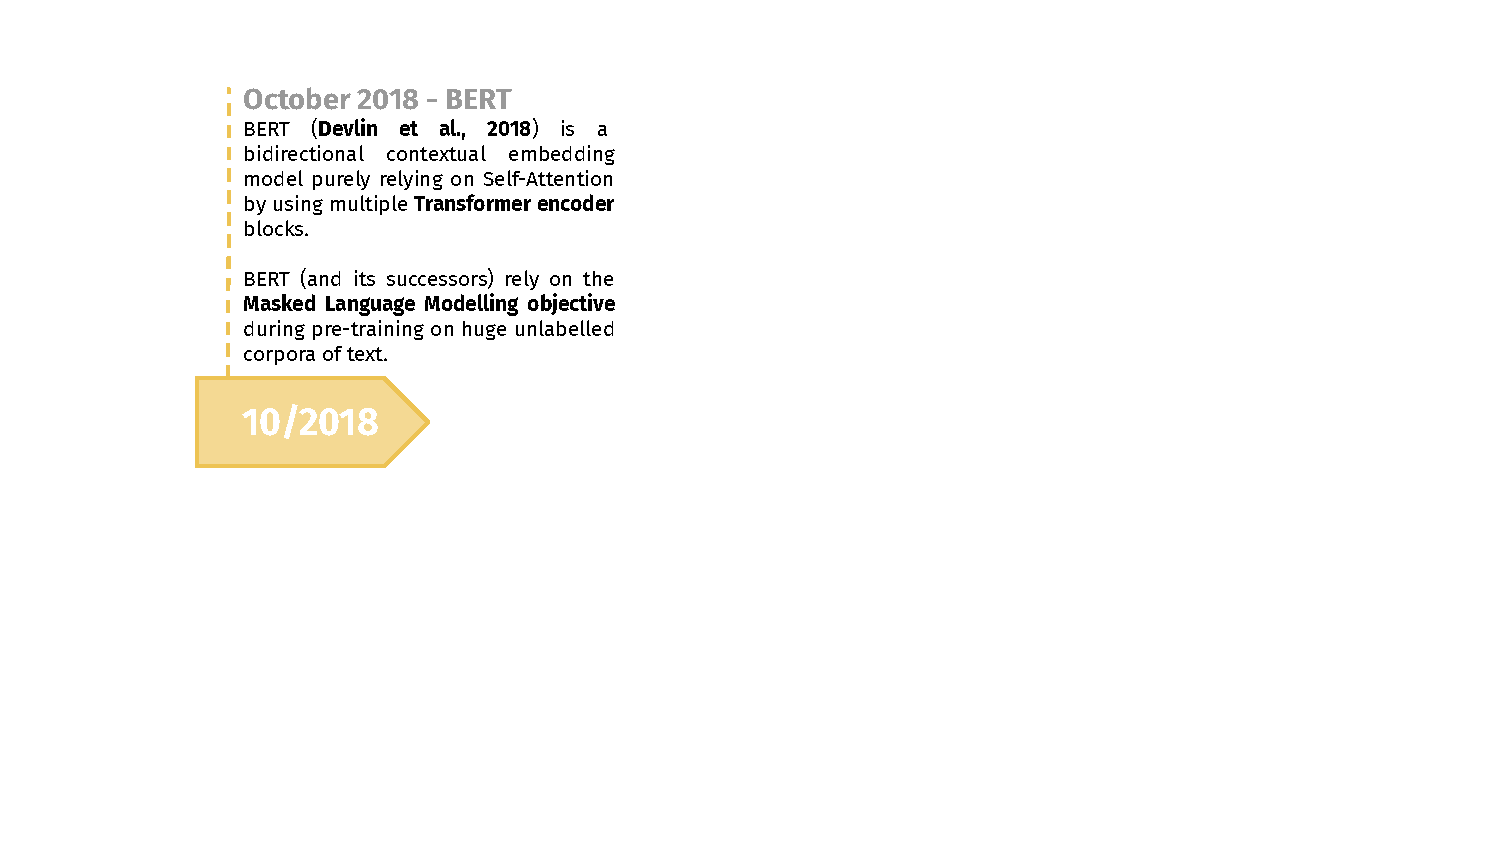
\includegraphics[width=12cm,page=1]{figure/transfer_learning_timeline4_nlp.pdf}}
\end{frame}
\begin{frame}[noframenumbering]{Successors of BERT}
\hbox{\hspace{-3em} \includegraphics[width=12cm,page=2]{figure/transfer_learning_timeline4_nlp.pdf}}
\end{frame}
\begin{frame}[noframenumbering]{Successors of BERT}
\hbox{\hspace{-3em} \includegraphics[width=12cm,page=3]{figure/transfer_learning_timeline4_nlp.pdf}}
\end{frame}
\begin{frame}[noframenumbering]{Successors of BERT}
\hbox{\hspace{-3em} \includegraphics[width=12cm,page=4]{figure/transfer_learning_timeline4_nlp.pdf}}
\end{frame}
\begin{frame}[noframenumbering]{Successors of BERT}
\hbox{\hspace{-3em} \includegraphics[width=12cm,page=5]{figure/transfer_learning_timeline4_nlp.pdf}}
\end{frame}

% ------------------------------------------------------------------------------

\begin{frame}{Different pre-training regimes (1)}

\vfill

	\textbf{ELECTRA} \citebutton{Clark et al, 2020}{https://arxiv.org/pdf/2003.10555.pdf}

	\begin{itemize}
		\item ELECTRA consinsts of two separate models
		\item[$\to$] (Small) generator model $G$ + (large) Discriminator model $D$
		\item[$\to$] This might resemble a GAN setup, but they are not trained in an adversarial manner
		\item Generator task: Masked language modeling
		\item Discriminator task: \textit{Replaced token detection}
		\item[$\to$] Predict for each token, whether it is "original" or produced by $G$
		\item ELECTRA learns from \textit{all} of the tokens (not just from a small portion of 15\%, like e.g. BERT)
	\end{itemize}
	
\vfill

\end{frame}

% ------------------------------------------------------------------------------

\begin{frame}{ELECTRA -- architecture}
	
\vfill

	\textbf{Joint pre-training:}
	
	\begin{figure}
		\centering
		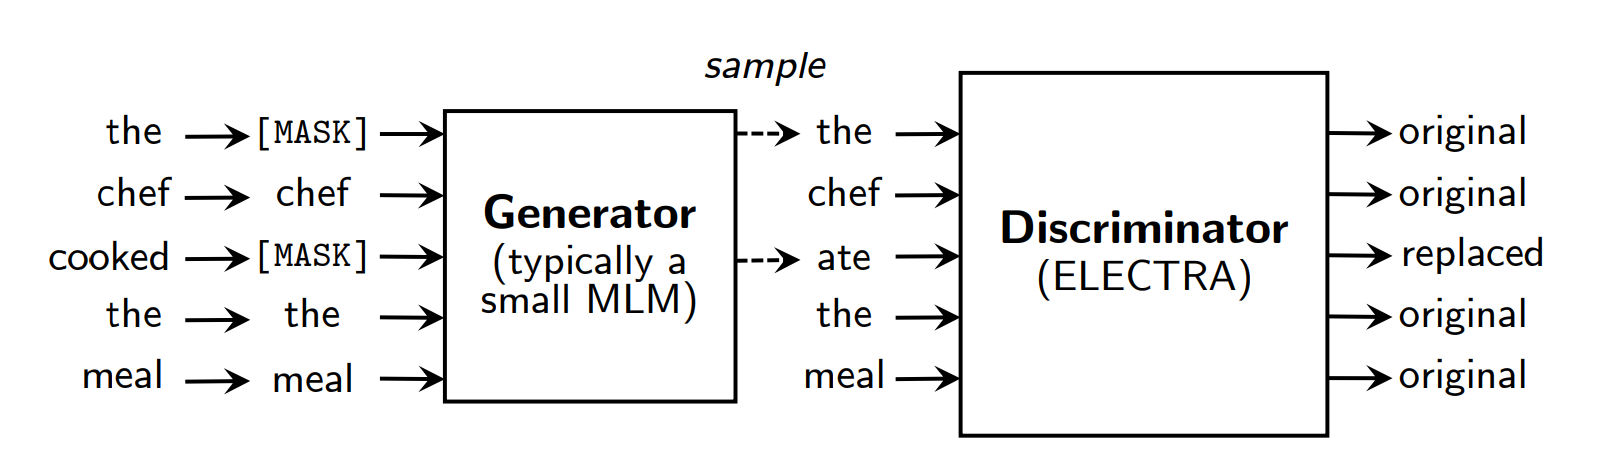
\includegraphics[width = 11cm]{figure/61-electra.png}\\ 
		\citebutton{Source: Clark et al, 2020}{https://arxiv.org/pdf/2003.10555.pdf}
	\end{figure}	
	
	\begin{itemize}
		\item $G$ and $D$ are (Transformer) encoders which are trained jointly
		\item $G$ replaces \texttt{[MASK]}s in an input sequence\\
					$\rightarrow$ Passes corrupted input sequence $\vec{x}^{corrupt}$ to $D$	
	\end{itemize}

\vfill

\end{frame}

% ------------------------------------------------------------------------------

\begin{frame}{ELECTRA -- Training details}

\vfill

	\textbf{Joint pre-training:}

	\begin{itemize}
		\item Generation of samples:
	\begin{figure}
		\centering
		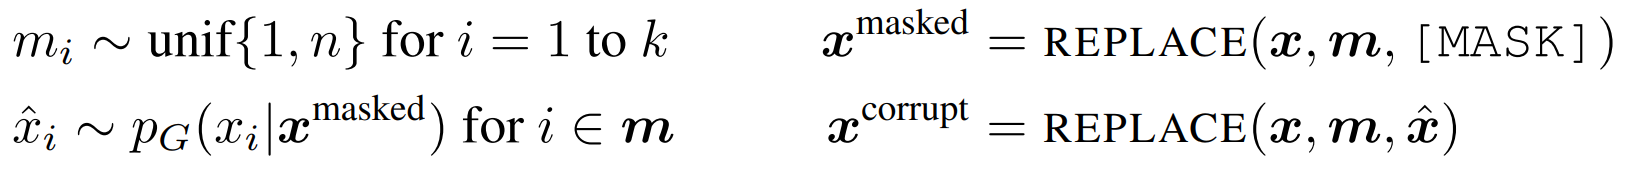
\includegraphics[width = 11cm]{figure/61-electra-samples.png}
	\end{figure}\vspace{-.25cm}
		{\footnotesize with approx. 15\% of the tokens masked out (via choice of $k$)}
		\item[]
		\item $D$ predicts whether $x_t,\; t \in 1, \hdots, T$ is "\textit{real}" or generated by $G$
			\begin{itemize}
				\item Softmax output layer for $G$ (probability distr. over all words)
				\item Sigmoid output layer for $D$ (Binary classification real vs. generated)
			\end{itemize}
	\end{itemize}
	
\vfill

\end{frame}

% ------------------------------------------------------------------------------

\begin{frame}{ELECTRA -- Training details}

\vfill

	Using the masked \& corrupted input sequences, the (joint) loss can be written down as follows:\\
	\vspace{.3cm}
	\textbf{Loss functions:}
	\begin{figure}
		\centering
		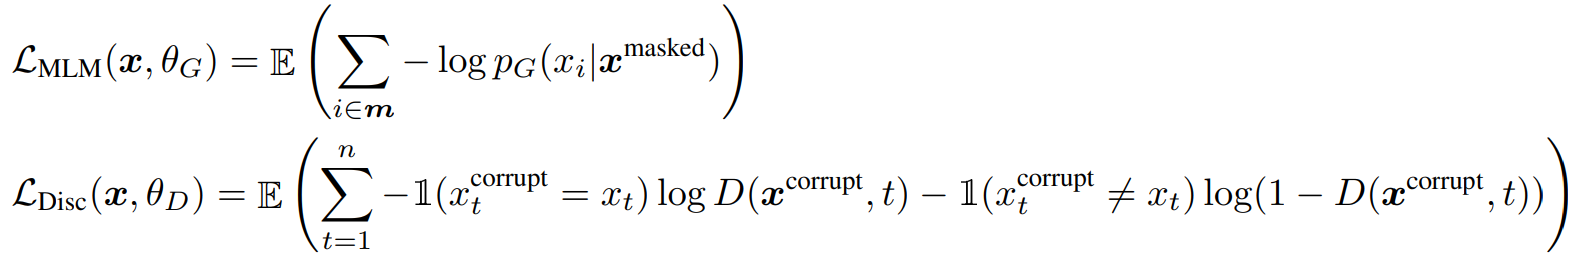
\includegraphics[width = 11cm]{figure/61-electra-loss.png}
	\end{figure}
	
	\textbf{Combined:}
	\begin{figure}
		\centering
		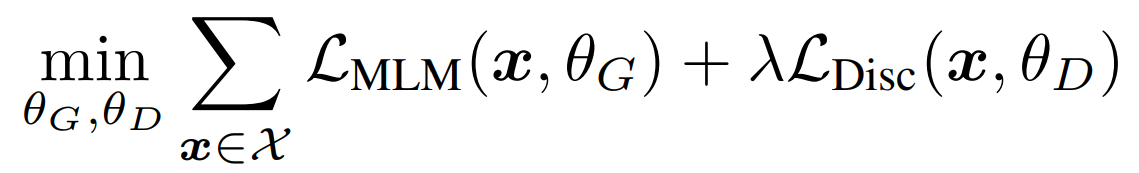
\includegraphics[width = 6cm]{figure/61-electra-loss-comb.png}
	\end{figure}
	{\footnotesize with $\lambda$ set to 50, since the discriminator's loss is typically much lower than the geneator's.}
	
\vfill

\end{frame}

% ------------------------------------------------------------------------------

\begin{frame}{ELECTRA -- Training details}

\vfill

	\textbf{Generator size:}

	\begin{itemize}
		\item Same size of $G$ and $D$: 
			\begin{itemize}
				\item Twice the compute per training step + too challenging for $D$
			\end{itemize}
		\item Smaller Generators are preferable (1/4 -- 1/2 the size of $D$)
	\begin{figure}
		\centering
		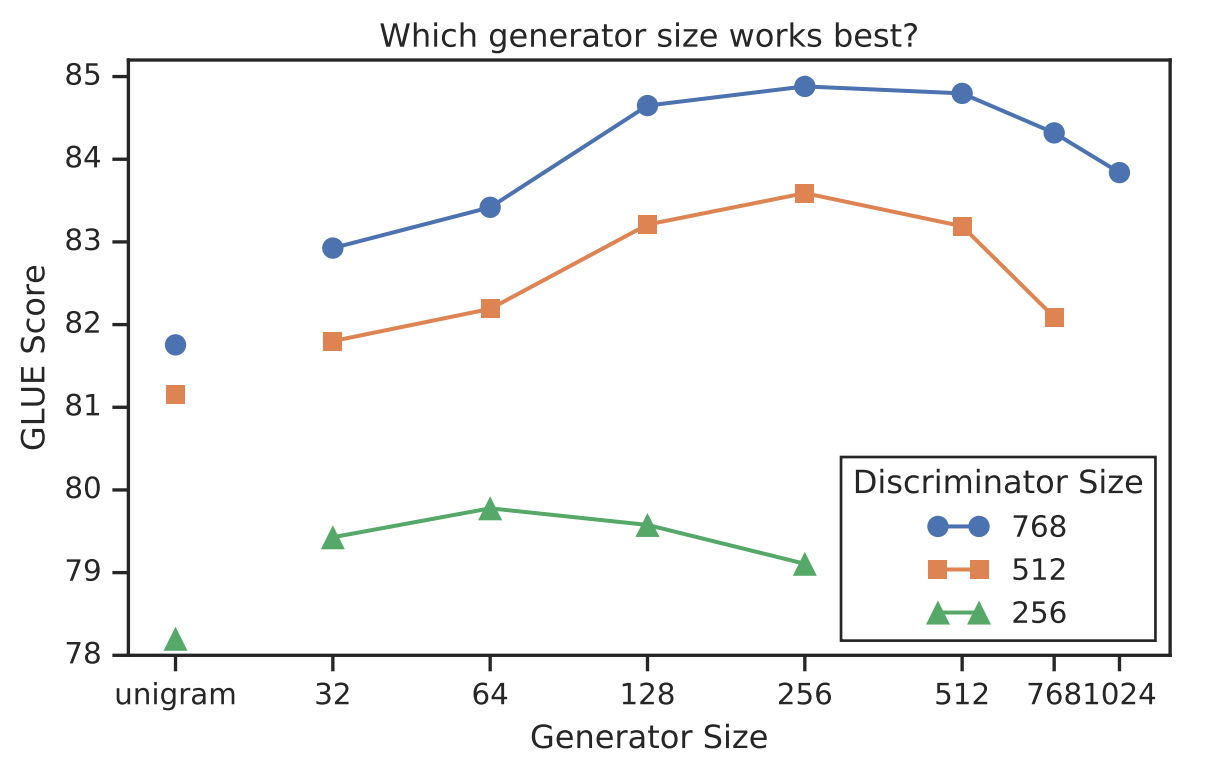
\includegraphics[width = 5cm]{figure/61-electra-size-g.png}\\ 
		\citebutton{Source: Clark et al, 2020}{https://arxiv.org/pdf/2003.10555.pdf}
	\end{figure}
	\end{itemize}
	
	\textbf{Weight sharing (experimental):}

	\begin{itemize}
		\item Same size of $G$ and $D$: All weights can be tied
		\item $G$ smaller than $D$: Share token \& positional embeddings 
	\end{itemize}
	
\vfill

\end{frame}

% ------------------------------------------------------------------------------

\begin{frame}{ELECTRA -- Model comparison}
	
\vfill

	\begin{figure}
		\centering
		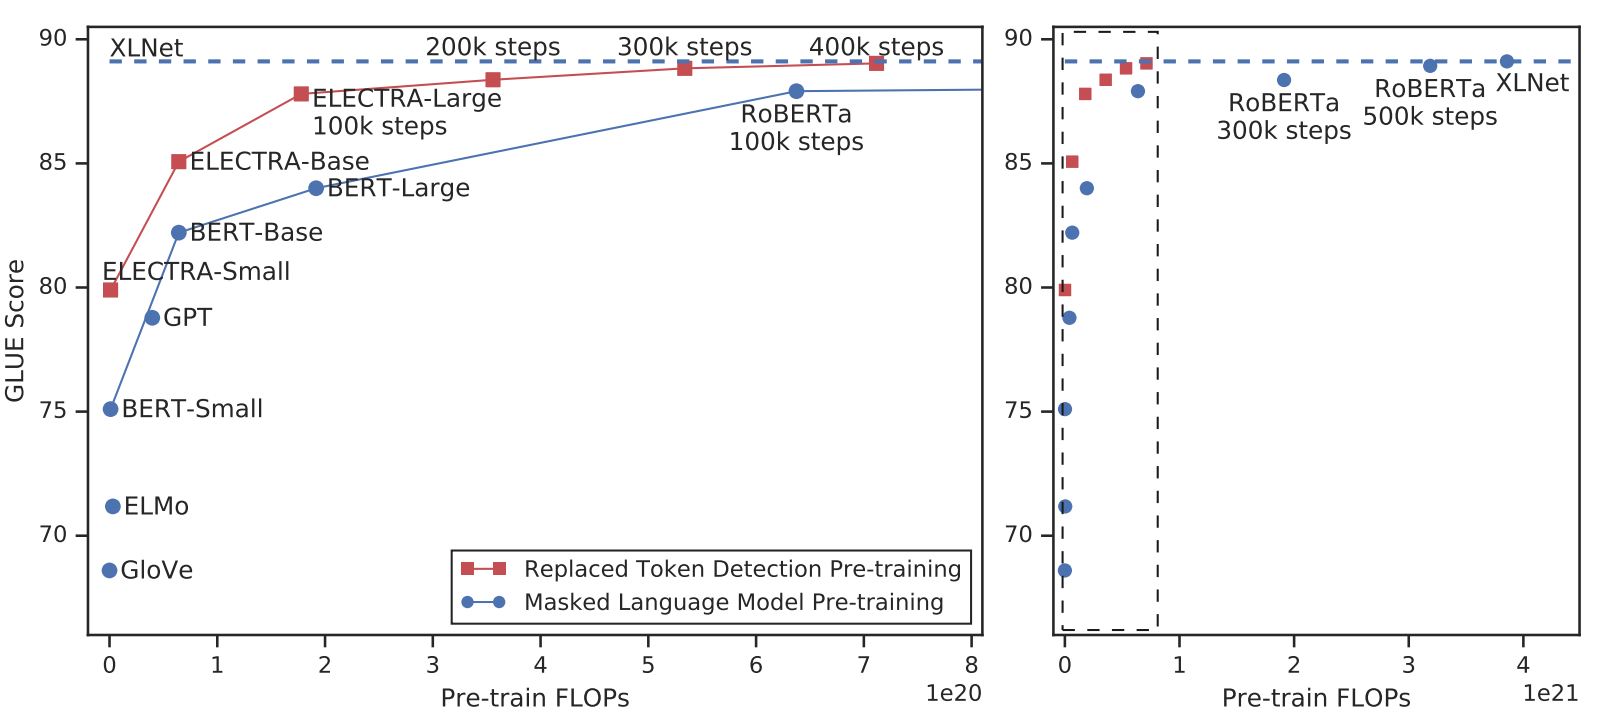
\includegraphics[width = 11cm]{figure/61-electra-glue.png}\\ 
		\citebutton{Source: Clark et al, 2020}{https://arxiv.org/pdf/2003.10555.pdf}
	\end{figure}
	
{\footnotesize \textit{Note:} Different batch sizes (2k vs. 8k) for ELECTRA vs. RoBERTa/XLNet explain why same number of steps lead to approx. 1/4 of the compute for ELECTRA.}

\vfill

\end{frame}

% ------------------------------------------------------------------------------

\begin{frame}{ELECTRA -- SOTA performance}

\vfill

	\textbf{Performance differences vs. BERT/RoBERTa (GLUE dev set):}

	\begin{figure}
		\centering
		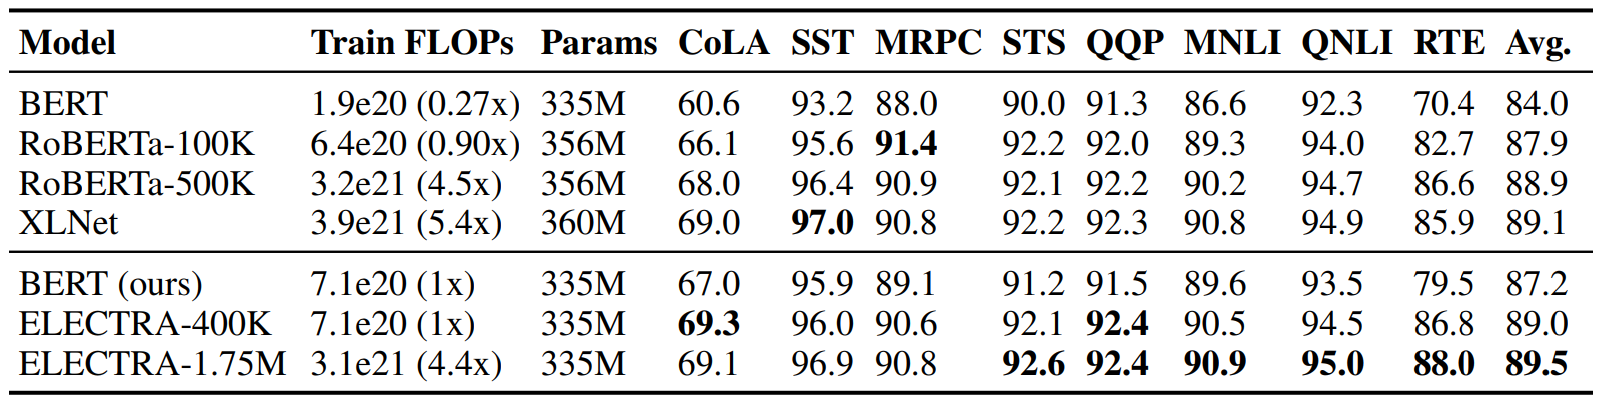
\includegraphics[width = 9cm]{figure/61-electra-sota1.png}\\ 
		\citebutton{Source: Clark et al, 2020}{https://arxiv.org/pdf/2003.10555.pdf}
	\end{figure}

	\textbf{SOTA performance (GLUE test set):}

	\begin{figure}
		\centering
		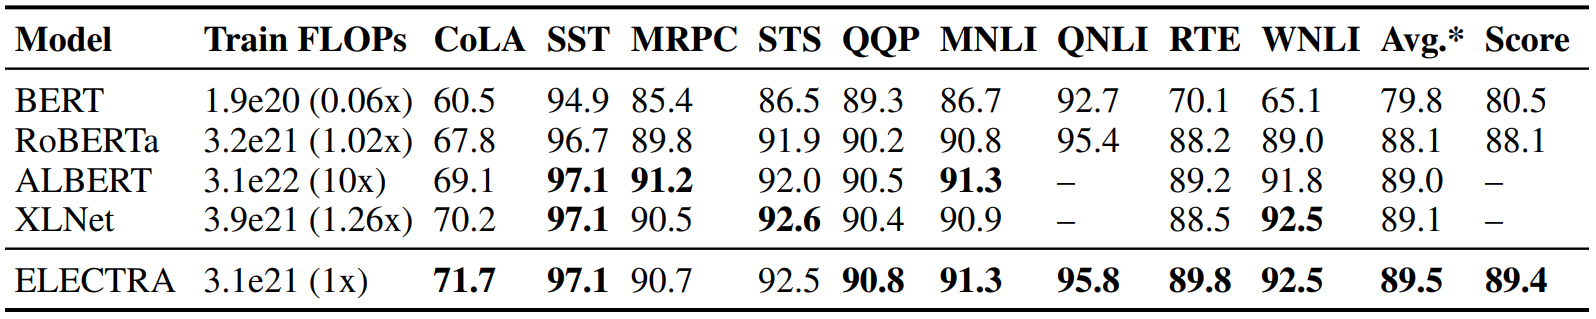
\includegraphics[width = 9cm]{figure/61-electra-sota2.png}\\ 
		{\tiny * Avg. excluding QNLI to ensure comparability}\\
		\citebutton{Source: Clark et al, 2020}{https://arxiv.org/pdf/2003.10555.pdf}
	\end{figure}
	
\vfill

\end{frame}

% ------------------------------------------------------------------------------

\begin{frame}{Different pre-training regimes (2)}

\vfill

	\textbf{Autoregressive (AR) language modeling}
	
	\begin{itemize}
		\item Factorizes likelihood to $$p(\mathbf{x}) = \prod_{t=1}^{T} p(x_t | \mathbf{x}{< t})$$
		\item Only uni-directional (backward factorization also possible)
	\end{itemize}

	\textbf{vs. (Denoising) Autoencoding (AE)}
	
	\begin{itemize}
		\item Reconstruct masked tokens $\bar{\mathbf{x}}$ from corrupted sequence $\hat{\mathbf{x}}$:
					$$p(\bar{\mathbf{x}}|\hat{\mathbf{x}}) = \prod_{t=1}^{T} m_t \cdot p(x_t | \hat{\mathbf{x}}), \text{with $m_t$ as masking indicator}$$
		\item Possible "\textit{corruptions}" (besides MLM):
		\item[] $\to$ Replacing words with predictions (cf. ELECTRA)
		\item[] $\to$ Shuffling tokens or dropping them
	\end{itemize}
	
\vfill

\end{frame}

% ------------------------------------------------------------------------------

\begin{frame}{Different pre-training regimes (2)}

\vfill
	
	\textbf{Conceptual Differences}
	
	\begin{itemize}
		\item \textbf{AR:} No corruption of input sequences required
		\item ``Causal`` structure in AR approach (sometimes needed)
		\item \textbf{AE:} Assumes independence between corrupted tokens
		\item[] \ques \textbf{Why?}
		\item AR approach only conditions on left side context
		\item[] $\to$ No bidirectionality possible
	\end{itemize}
	
\vfill

\end{frame}

% ------------------------------------------------------------------------------

\begin{frame}{Permutation language modeling (PLM)}

\vfill

	\textbf{XLNet} \citebutton{Yang et al., 2019}{https://papers.nips.cc/paper/8812-xlnet-generalized-autoregressive-pretraining-for-language-understanding.pdf}
	
	\begin{itemize}
		\item Alternative objective function
		\item Solves the pretrain-finetune discrepancy
		\item[$\to$] No artificial \texttt{[MASK]} token is introduced
		\item Allows for bidirectionality while keeping an AR objective
		\item[$\to$] Best of both worlds
		\item Consists of two "\textit{streams}" of the Attention mechanism
				\begin{itemize}
					\item Content-stream attention
					\item Query-stream attention
				\end{itemize}
	\end{itemize}
	
\vfill

\end{frame}

% ------------------------------------------------------------------------------

\begin{frame}{Permutation language modeling (PLM)}

\vfill
	
	\textbf{Manipulating the factorization order}
	
	\begin{itemize}
		\item Consider permutations $\mathbf{z}$ of the index sequence $[1,2, \hdots, T]$
		\item[$\to$] Used to permute the factorization order, \textit{not} the sequence order.
		\item Original order of the sequence is retained via positional encodings
		\item PLM objective (with $\mathcal{Z}_T$ as set of all possible permutations):
					$$\max_{\theta} \quad \mathds{E}_{\mathbf{z}\sim\mathcal{Z}_T} \left[ \sum_{t=1}^{T} \log p_\theta (x_{z_t} | \mathbf{x}_{\mathbf{z}_{< t}}) \right]$$
	\end{itemize}
	
\vfill

\end{frame}

% ------------------------------------------------------------------------------

\begin{frame}{plm -- content- vs. query-stream}

\vfill

	\textbf{Content-stream}
	
	\begin{itemize}
		\item ``Ordinary`` Self-Attention (with special attention masks)\\
					$\rightarrow$ Attentions masks depend on the factorization order
		\item Information about the position in the sequence is lost,\\
					see \citebutton{Example in A.1 (Yang et al., 2019)}{https://arxiv.org/abs/1906.08237}
		\item Sets of queries ($Q$), keys ($K$) and values ($V$) from content stream*
		\item Yields a \textit{content embedding} denoted as $h_{\theta}(\mathbf{x}_{\mathbf{z}_{\leq t}})$
	\end{itemize}
	
\vfill

	{\footnotesize *For a nice visual disentanglement, see \citebutton{Figures in A.7 (Yang et al., 2019)}{https://arxiv.org/abs/1906.08237}}
	
\end{frame}

% ------------------------------------------------------------------------------

\begin{frame}{plm -- content- vs. query-stream}

\vfill

	\textbf{Content-stream}
	
	\begin{figure}
		\centering
		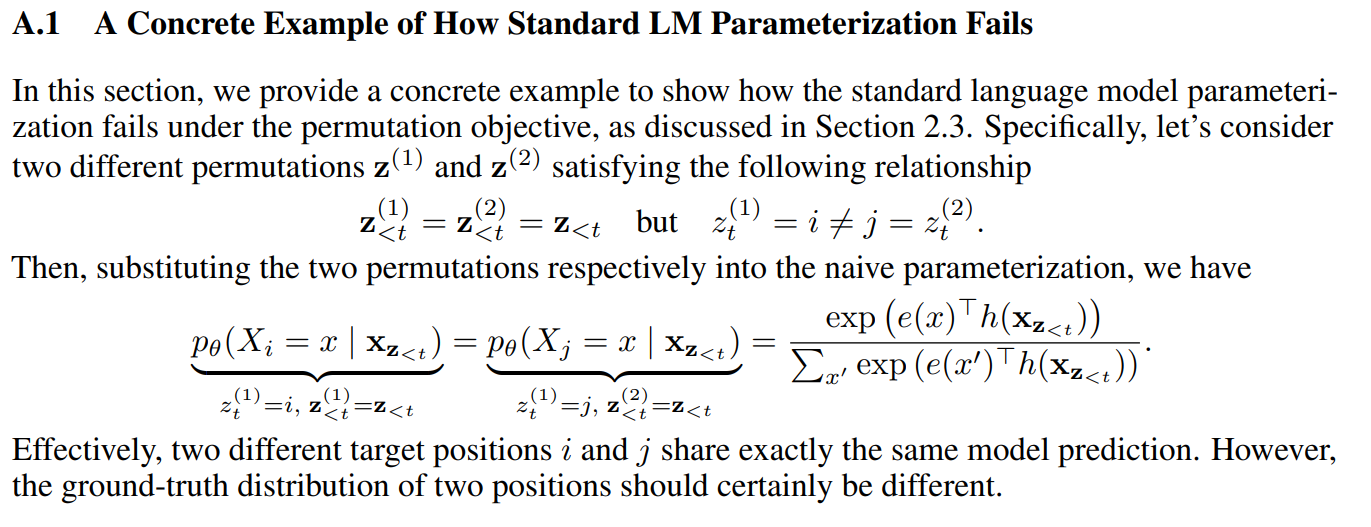
\includegraphics[width = 10cm]{figure/61-xlnet-a1.png}\\ 
		\citebutton{Source: Yang et al., 2019}{https://papers.nips.cc/paper/8812-xlnet-generalized-autoregressive-pretraining-for-language-understanding.pdf}
	\end{figure}
	
\vfill

\end{frame}

% ------------------------------------------------------------------------------

\begin{frame}{plm -- content- vs. query-stream}

\vfill
	
	\textbf{Query-stream}
	
	\begin{itemize}
		\item Access to context through content-stream, but no access to the content of the current position (only location information)
		\item $Q$ from the query stream, $K$ and $V$ from the content stream*
		\item Yields a \textit{query embedding} denoted as $g_{\theta}(\mathbf{x}_{\mathbf{z}_{< t}}, z_t)$
	\end{itemize}

\vfill

	{\footnotesize *For a nice visual disentanglement, see \citebutton{Figures in A.7 (Yang et al., 2019)}{https://arxiv.org/abs/1906.08237}}
	
\end{frame}

% ------------------------------------------------------------------------------

\begin{frame}{plm -- content- vs. query-stream}

\vfill

	\textbf{Content-stream}
	
	\begin{figure}
		\centering
		\hspace{-2cm}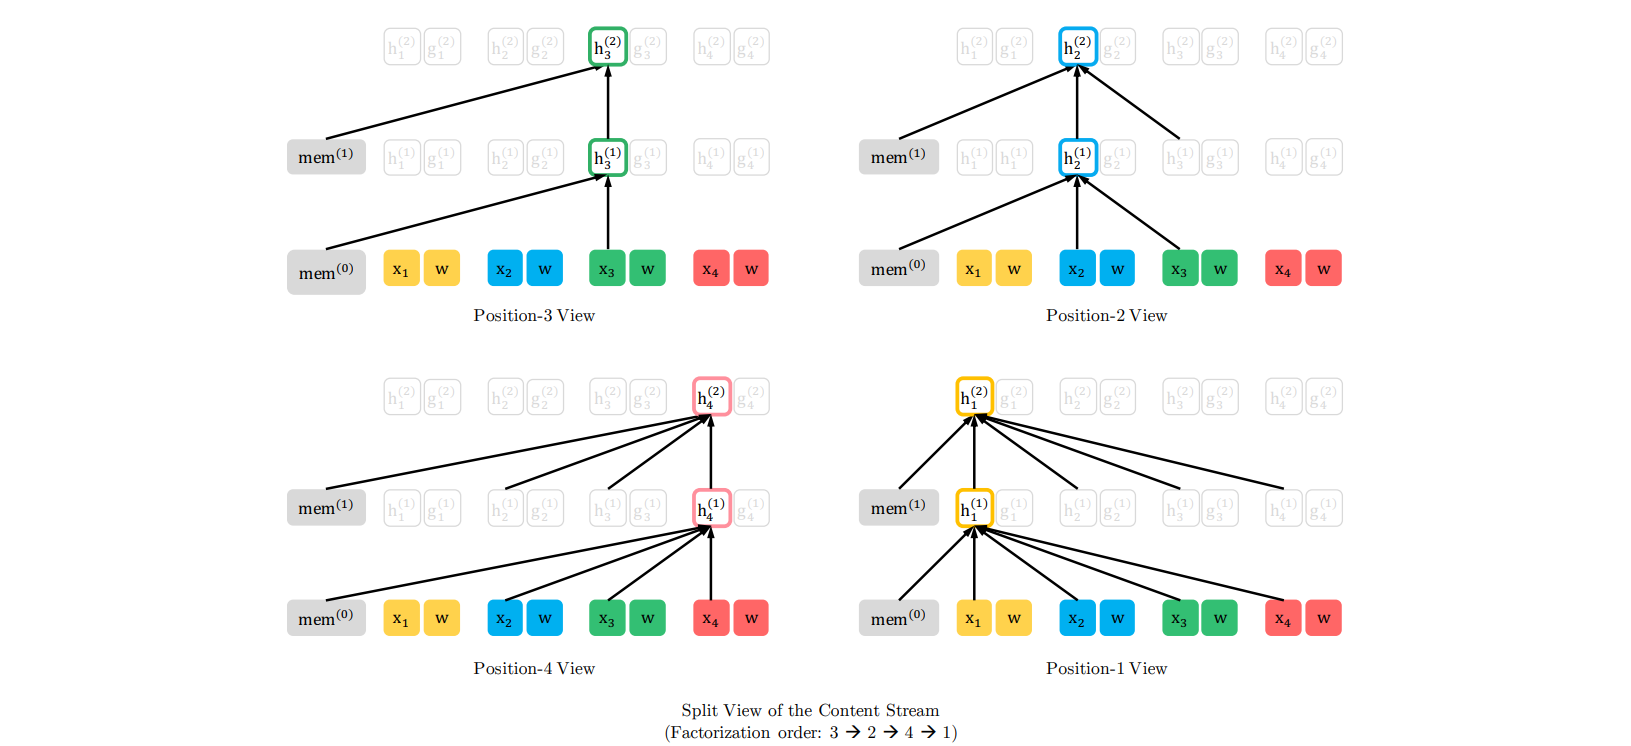
\includegraphics[width = 13cm]{figure/61-xlnet-content.png}\\ 
		\citebutton{Source: Yang et al., 2019}{https://papers.nips.cc/paper/8812-xlnet-generalized-autoregressive-pretraining-for-language-understanding.pdf}
	\end{figure}
	
\vfill

\end{frame}

% ------------------------------------------------------------------------------

\begin{frame}{plm -- content- vs. query-stream}

\vfill

	\textbf{Query-stream}
	
	\begin{figure}
		\centering
		\hspace{-2cm}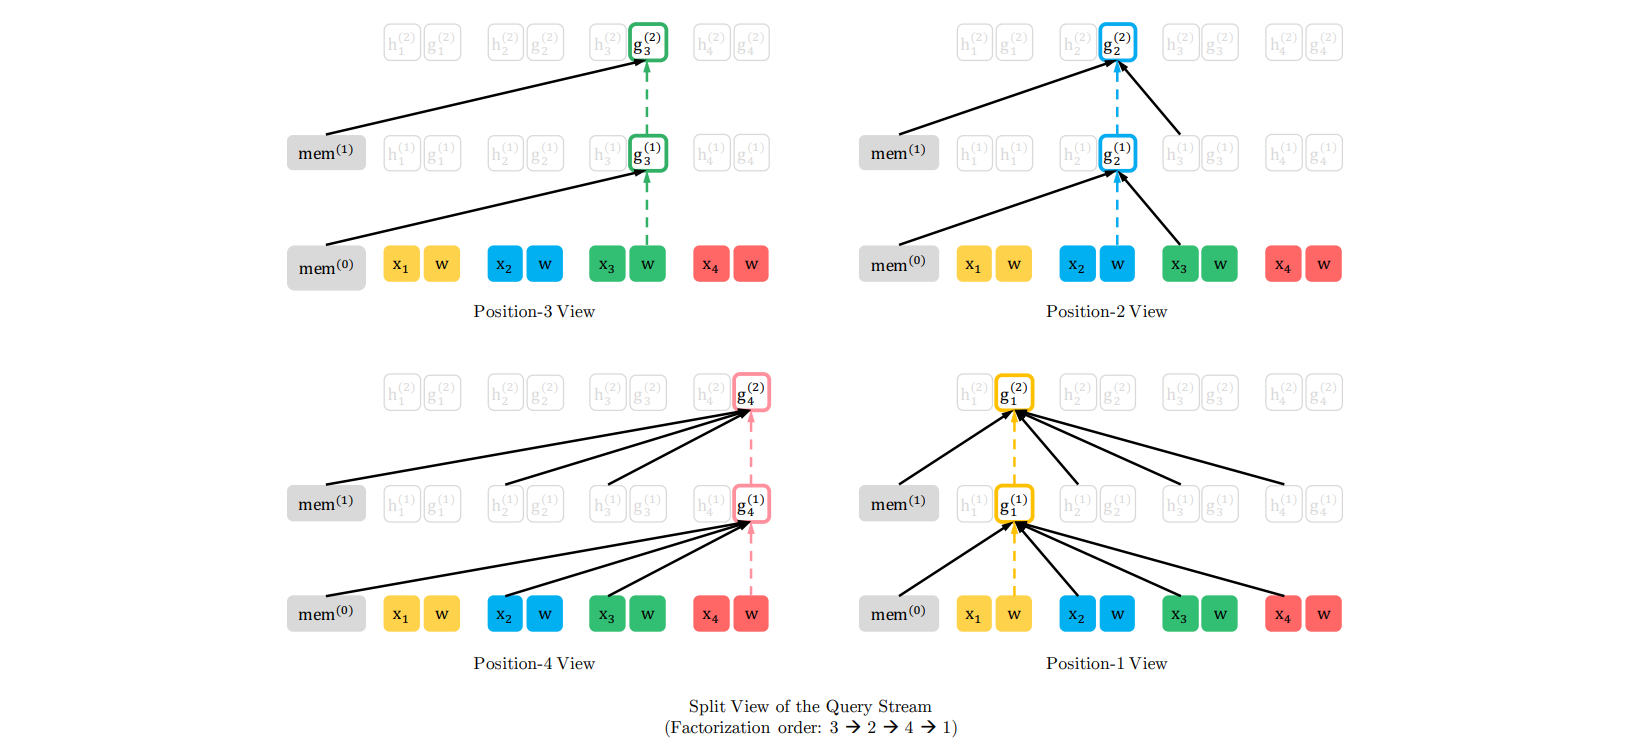
\includegraphics[width = 11.05cm]{figure/61-xlnet-query.png}\\ 
		\citebutton{Source: Yang et al., 2019}{https://papers.nips.cc/paper/8812-xlnet-generalized-autoregressive-pretraining-for-language-understanding.pdf}
	\end{figure}
	
\vfill

\end{frame}

% ------------------------------------------------------------------------------

\begin{frame}{plm -- content- vs. query-stream}

\vfill

	\begin{figure}
		\centering
		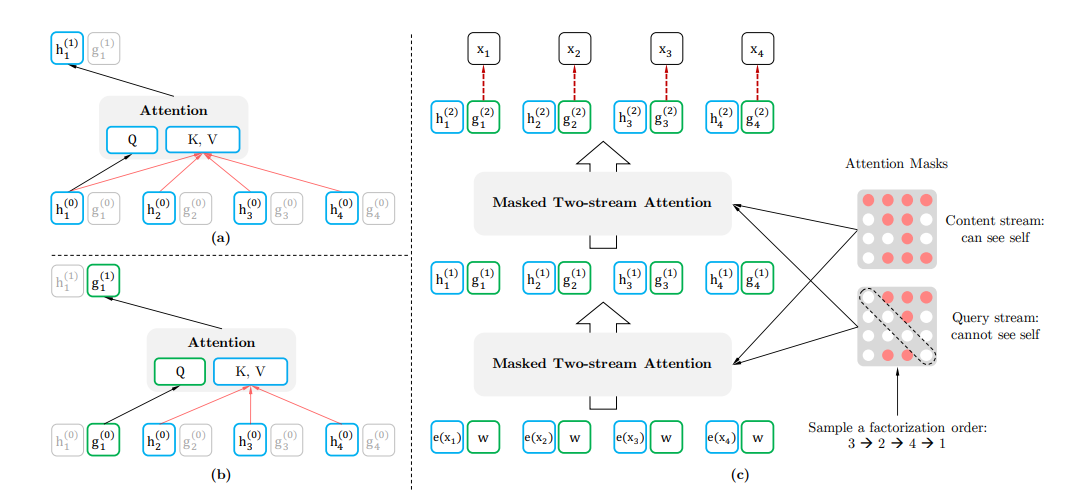
\includegraphics[width = 10.20cm]{figure/61-xlnet}\\ 
		{\tiny (a) content-stream; (b) query-stream; (c) whole model}\\
		\citebutton{Source: Yang et al., 2019}{https://papers.nips.cc/paper/8812-xlnet-generalized-autoregressive-pretraining-for-language-understanding.pdf}
	\end{figure}
	
\vfill

\end{frame}

% ------------------------------------------------------------------------------

\begin{frame}{XLNet -- Model Input}

\vfill

\textbf{Generation of samples:}

\begin{itemize}
\item Randomly sample two sentences and use concatenation* as input
			{\footnotesize
\begin{center}
\begin{tabular}{|cccccccc|}
\hline
\cellcolor{blue!15}\texttt{[CLS]} & The & fox & is & quick & . & \cellcolor{blue!15}\texttt{[SEP]} &\\\hline\hline It & jumps & over & the & lazy & dog & . & \cellcolor{blue!15}\texttt{[SEP]} \\
\hline
\end{tabular}\\\mbox{}
\end{center}}
{\scriptsize *Nevertheless: XLNet does \textit{not} use the NSP objective }
\end{itemize}

\textbf{Additional encodings:}

\begin{itemize}
\item \textit{Relative} segment encodings:
	\begin{itemize}
		\item BERT adds absolute segment embeddings ($E_A$ \& $E_B$)
		\item XLNet uses relative encodings ($\vec{s}_+$ \& $\vec{s}_-$)
	\end{itemize}
\item \textit{Relative} Positional encodings:
	\begin{itemize}
		\item BERT encodes information about the absolute position ($E_0, E_1, E_2, \hdots$)
		\item XLNet uses relative encodings ($R_{i - j}$)
	\end{itemize}
\end{itemize}

\vfill

\end{frame}

% ------------------------------------------------------------------------------

\begin{frame}{XLNet -- Special remarks}
	
\vfill

	\begin{itemize}
		\item \textbf{Partial Prediction:} Only predict the last tokens in a factoriztion order (reduces optimization difficulty)
					{\small $$\max_{\theta} \quad \mathds{E}_{\mathbf{z}\sim\mathcal{Z}_T} \left[ \sum_{t=c+1}^{|\mathbf{z}|} \log p_\theta (x_{z_t} | \mathbf{x}_{\mathbf{z}_{< t}}) \right],\quad \mbox{with $c$ as cutting point}$$}
		\item \textbf{Segment recurrence mechanism:} Allow for learning extended contexts in Transformer-based architectures, see \citebutton{Dai et al. (2019)}{https://arxiv.org/pdf/1901.02860.pdf}
		\item \textbf{No independence assumption:}
	\begin{figure}
		\centering
		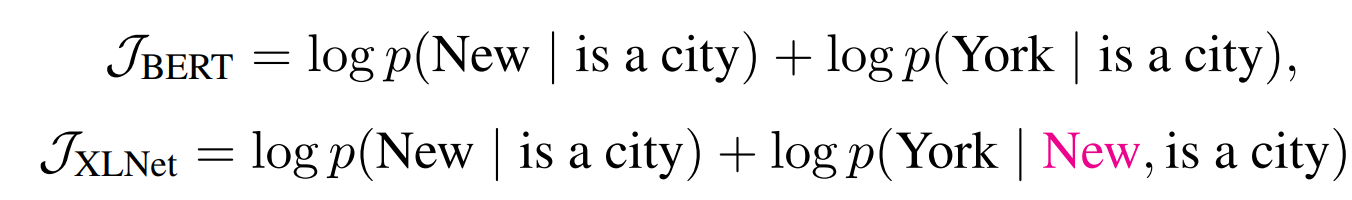
\includegraphics[width = 9cm]{figure/61-xlnet-objective}\\ 
		{\tiny Prediction of [New, York] given the factorization order [is, a, city, New, York]}\\
		\citebutton{Source: Yang et al., 2019}{https://papers.nips.cc/paper/8812-xlnet-generalized-autoregressive-pretraining-for-language-understanding.pdf}
	\end{figure}
	\end{itemize}
	
\vfill

\end{frame}

% ------------------------------------------------------------------------------

\begin{frame}{XLNet -- SOTA performance}

\vfill

	\textbf{Performance differences to BERT:}

	\begin{figure}
		\centering
		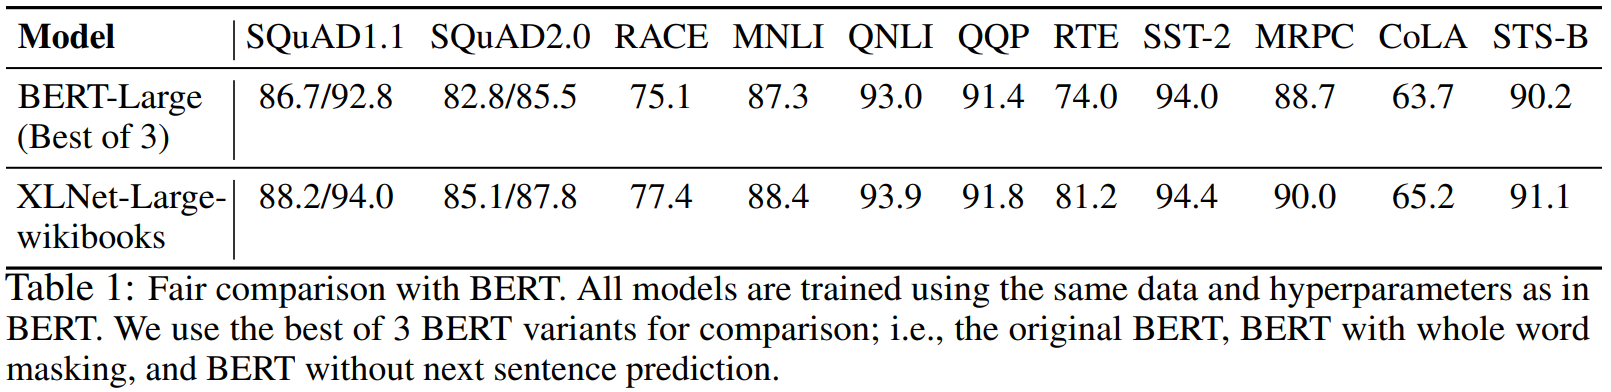
\includegraphics[width = 7.65cm]{figure/61-xlnet-vs-bert.png}\\ 
		\citebutton{Source: Yang et al., 2019}{https://papers.nips.cc/paper/8812-xlnet-generalized-autoregressive-pretraining-for-language-understanding.pdf}
	\end{figure}

	\textbf{SOTA performance:}

	\begin{figure}
		\centering
		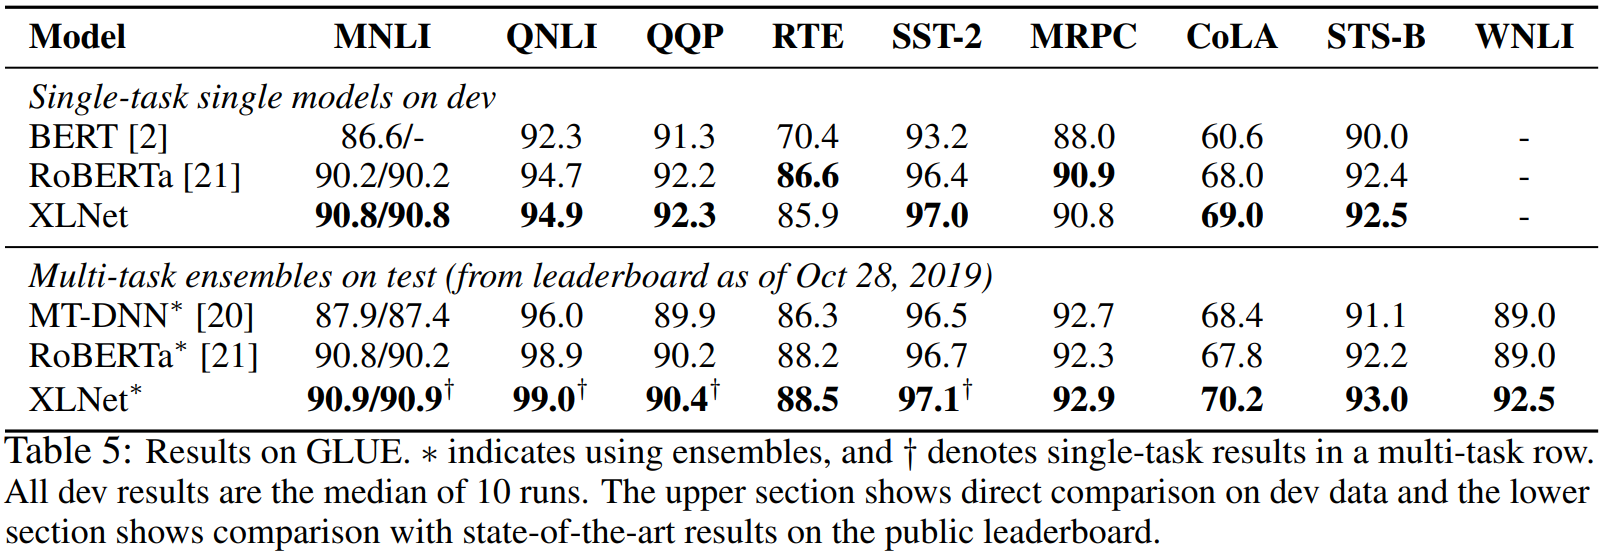
\includegraphics[width = 7.65cm]{figure/61-xlnet-sota.png}\\ 
		\citebutton{Source: Yang et al., 2019}{https://papers.nips.cc/paper/8812-xlnet-generalized-autoregressive-pretraining-for-language-understanding.pdf}
	\end{figure}
	
\vfill

\end{frame}

% ------------------------------------------------------------------------------


%%%%%%%%%%%%%%%%%%%%%%%%%%%%%%%%%%%%%%%%%%%%%%%%%%%%%%%%%%%%%%%%%%
\section{Tasks as Text-to-Text Problem}
% Source: DL4NLP chapter06-post-bert-t5/slides-62-text2text.tex
%%%%%%%%%%%%%%%%%%%%%%%%%%%%%%%%%%%%%%%%%%%%%%%%%%%%%%%%%%%%%%%%%%
% ------------------------------------------------------------------------------

\begin{frame}{Recap: BERT, RoBERTa, etc.}

\vfill

  \begin{itemize}
\item Transformer encoder
\item Training: Masked language modeling (or similar)
\item BERT* learns an enormous amount of knowledge
about language and the world through MLM training on large corpora
\item Application: fine-tune on a particular task
\item Great performance!
\item \ques What's not to like?
    \end{itemize}

\vfill

*\scriptsize{In what follows we will use BERT as a representative for this class of language models, i.e. models with a custom classification layer of each task, and only talk about BERT -- but the discussion includes RoBERTa, Albert, XLNet etc.}

\end{frame}

% ------------------------------------------------------------------------------

\begin{frame}{Problems with BERT (1)}

\vfill

  \begin{itemize}
\item You need a different model for each task.
\item[] (Because BERT is differently fine-tuned for each task.)
\item[] $\to$ Not realistic in many real deployment scenarios, e.g., on mobile devices.
\item \textit{Human learning:} We arguably have a \myblue{single} model that solves all tasks!
\item \ques Is there a framework that allows us to create a single model that solves all tasks?
    \end{itemize}

\vfill

\end{frame}

% ------------------------------------------------------------------------------

\begin{frame}{Problems with BERT (2)}

\vfill
			
\begin{itemize}
\item Two training modes: first (MLM) pretraining, then fine-tuning.
\item Fine-tuning is \myblue{supervised learning}, i.e., learning from labeled examples.
\item Arguably, learning from labeled examples is untypical for human learning.
\item You never learn a task solely by being presented a bunch of examples, without explanation.
\item Instead, in human learning, there is almost always a \myblue{task description}.
    \end{itemize}

\vfill

\end{frame}

% ------------------------------------------------------------------------------

\begin{frame}{Problems with BERT (2)}

\vfill
			
\begin{itemize}
\item Example: \textit{How to boil an egg.}
		\begin{itemize}
			\item ``Place eggs in the bottom of a saucepan.``
			\item ``Fill the pan with cold water.``
			\item ``Etc.``
		\end{itemize}
\item Notice that this is \myblue{not} an example but a \textit{description} of the task
\item \ques Is there a framework that allows us to leverage task descriptions?
\end{itemize}

\vfill

\end{frame}

% ------------------------------------------------------------------------------

\begin{frame}{Problems with BERT (3)}

\vfill

  \begin{itemize}
\item BERT has great performance, but \ldots
\item \ldots only if the training set is large, generally 1000s of examples
\item This is completely different from human learning!
\item We do use examples in learning, but in most cases, only a few
\end{itemize}

\vfill

\end{frame}

% ------------------------------------------------------------------------------

\begin{frame}{Problems with BERT (3)}

\vfill

  \begin{itemize}
\item Example: Maybe the person teaching you how to boil an egg will show you how to do it \textit{one or two times}
\item But probably \myblue{not} 10 times
\item Definitely \myblue{not} a 1000 times 
\item More practical concern: it's very expensive to label 1000s of examples for each task (there are many tasks).
\item \ques Is there a framework that allows us to learn from just a small number of examples?
\item This is called \myblue{few-shot learning}.
    \end{itemize}

\vfill

\end{frame}

% ------------------------------------------------------------------------------

\begin{frame}{Problems with BERT (4)}

\vfill

  \begin{itemize}
		\item More subtle aspect of the same problem (i.e., large training sets):
		\item[] $\to$ \textbf{Overfitting}
		\item Even though performance looks good on standard train/dev/test splits, the deviation between the training set and the
data actually encountered in real application can be large
		\item So our benchmarks often overestimate what performance would be in reality
  \end{itemize}

\vfill

\end{frame}

% ------------------------------------------------------------------------------

\begin{frame}{Problems with BERT -- summary}

\vfill

  \begin{itemize}
		\item No true multitask learning
		\item Differs from the way humans learn
		\item No possibility/necessity to make use of a description of the task
		\item Overfitting
  \end{itemize}

\vfill

\end{frame}

% ------------------------------------------------------------------------------

\begin{frame}{revisiting text-to-text tasks}

\vfill

\textbf{Example: Machine Translation}
	
	\begin{figure}
		\centering
		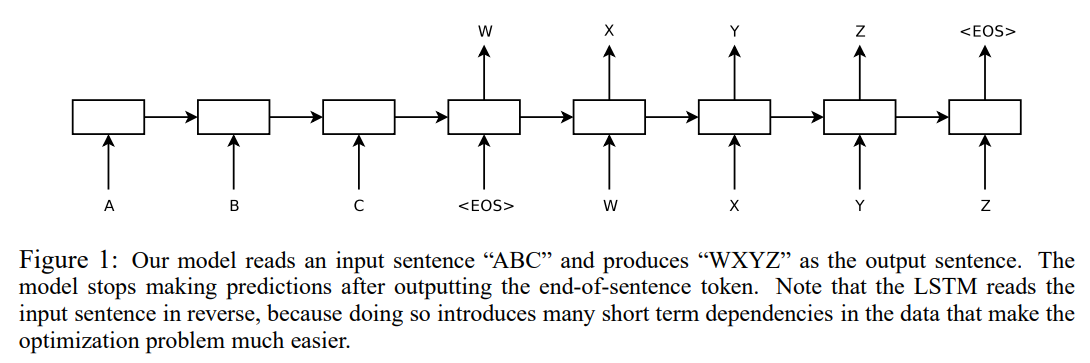
\includegraphics[width = 11cm]{figure/seq2seq.png}\\ 
	\citebutton{Source: Sutskever et al., 2014}{https://arxiv.org/pdf/1409.3215.pdf}
	\end{figure}

\begin{itemize}
	\item \textit{Input:} Text in source language
	\item \textit{Output:} Text in target language
\end{itemize}

\vfill

\end{frame}

% ------------------------------------------------------------------------------

\begin{frame}{revisiting fine-tuning of bert}

\vfill

	\begin{figure}
	\centering
		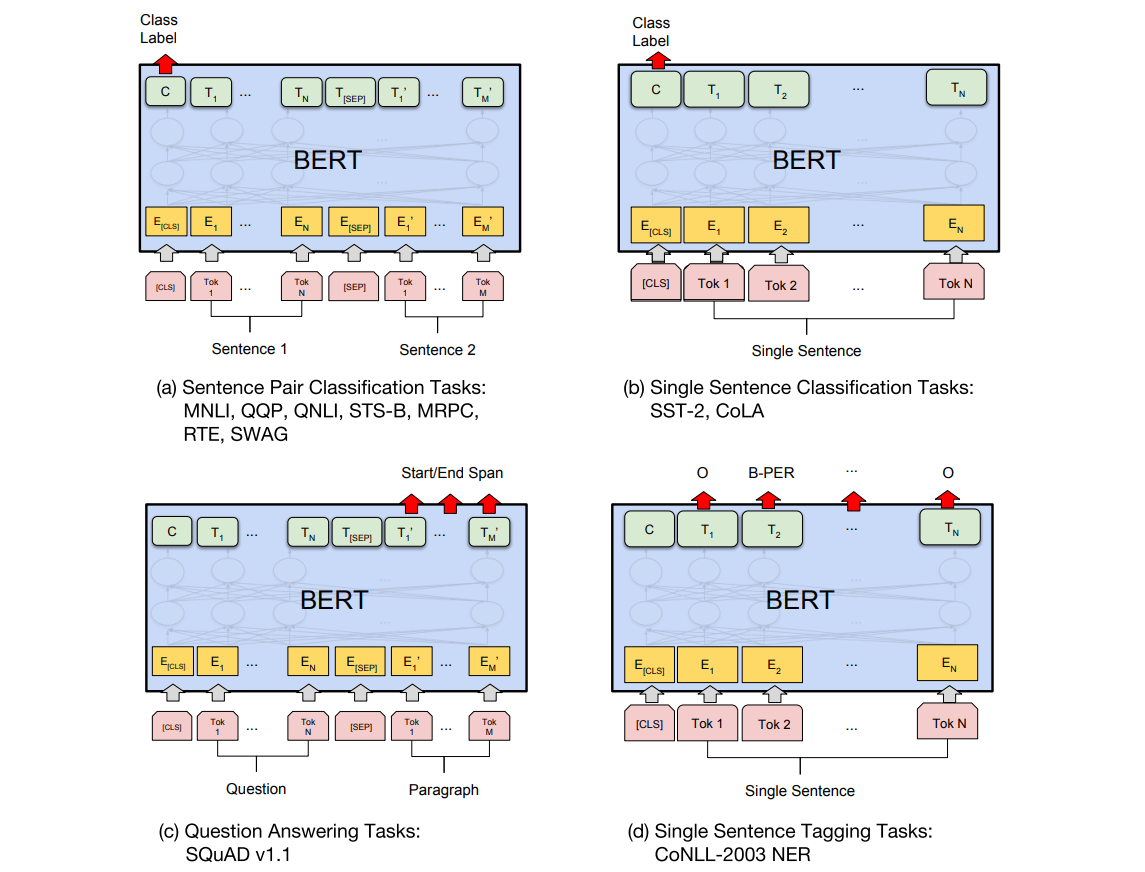
\includegraphics[width = 6.80cm]{figure/bert-finetune.png}\\ 
	\citebutton{Source: Devlin et al., 2019}{https://aclanthology.org/N19-1423.pdf}
	\end{figure}
	
\begin{itemize}
	\item \textit{First row:} (sequence-level) classification
	\item \textit{Second row:} sequence tagging = token-level classification
\end{itemize}

\vfill

\end{frame}

% ------------------------------------------------------------------------------

\begin{frame}{fine-tuning + text-to-text?}

\vfill

\begin{itemize}
	\item \ques How does BERT know which task it is performing?
			\begin{itemize}
				\item It doesn't!
				\item BERT just learns associations between text features and class distributions
				\item No meaningful internal representation of what ``class 3`` actually \textit{means}
				\item \textit{Input}: text; \textit{Output}: \texttt{[0 0 1 0 0 0]}
			\end{itemize}
	\item The fact that BERT does not ``understand`` what task it is actually performing is the reason why one copy is needed per task
\end{itemize}

\vfill

\end{frame}

% ------------------------------------------------------------------------------

\begin{frame}{fine-tuning + text-to-text?}

\vfill

\begin{itemize}
	\item \ques How could we ``inform`` our model about the task?
			\begin{itemize}
				\item Model takes text as an input and can process.
				\item Why not describe the task in natural language?
				\item \textit{Assumption:}\\
							Given the model sees 1000s of (inputs; ouput) pairs like ..
			\end{itemize}
\end{itemize}

		\begin{center}
				{\small
					(``\texttt{<task description>: <input sample>}`` ; ``\texttt{<class name>}``)
				}
		\end{center}
				
\begin{itemize}
			\item[]
			\begin{itemize}
				\item .. it will learn to associate ..
				\item[] $\to$ .. task descriptions to a set of class names
				\item[] $\to$ .. text features to class name distributions
			\end{itemize}
\end{itemize}

\vfill

\end{frame}

% ------------------------------------------------------------------------------

\begin{frame}{fine-tuning + text-to-text?}

\vfill

\begin{itemize}
	\item \ques How does a ``good`` task description look like?
			\begin{itemize}
				\item Remember: The idea is to have a model that learns to associate the task descriptions with a set of class names
				\item \textit{Class names:} 
				\item[] $\to$ Could be pretty new/exotic terms the model is not familiar with after pre-training
				\item[] $\to$ It will learn to output them during fine-tuning when ``triggered`` accordingly (i.e. with the right task description)
				\item \textit{Task descriptions:} 
				\item[] $\to$ Might be possible that the the model already saw some task descriptions during pre-training and has a meaningful representation for them.
				\item[] $\to$ On the other hand: Others might also be pretty new/exotic.
			\end{itemize}
\end{itemize}

\vfill

\end{frame}

% ------------------------------------------------------------------------------

\begin{frame}{fine-tuning + text-to-text?}

\vfill

For sentiment classification, I can just provide it with 1000s of training samples like 

		\begin{center}
				{\small
					(``\texttt{<sentiment classification>: <input sample>}`` ; ``\texttt{<positive/negative>}``)
				}
		\end{center}
		
The model will ..

\begin{itemize}
	\item .. utilize already present knowledge about the task description.
	\item .. learn to associate the task description precisely with this label set
\end{itemize}

\vfill

\end{frame}

% ------------------------------------------------------------------------------

\begin{frame}{fine-tuning + text-to-text?}

\vfill

\begin{itemize}
	\item \ques If I want the model to do sentiment classification, can I also just provide it with 1000s of training samples like 
\end{itemize}

		\begin{center}
				{\small
					(``\texttt{<khaleesi>: <input sample>}`` ; ``\texttt{<positive/negative>}``)
				}
		\end{center}
				
\begin{itemize}
	\item[] ? 
	\item[] (\textit{khaleesi}$^1$ just used as some random fantasy word here)
	\pause
	\item \textit{Intuition:} Yes! It basically does not matter, \textbf{as long as the model is fine-tuned on this data}$^2$
	\item Fine-tuning important for the model to pick up on this ``signal`` and output according text (corresponding the appropriate classes)
\end{itemize}

\vfill

$^1$\footnotesize{Khaleesi is a Dothraki title referring to the wife of the khal (cf. Game of Thrones).}\\
$^2$\footnotesize{Of course, using ``good`` task descriptions (as shown on the previous slide) that are also meaningful to human readers make more sense as the model might learn quicker because they diverge less from the pre-training distribution.}

\end{frame}

% ------------------------------------------------------------------------------

\begin{frame}{multi-task learning?}

\vfill

\begin{figure}
	\centering
		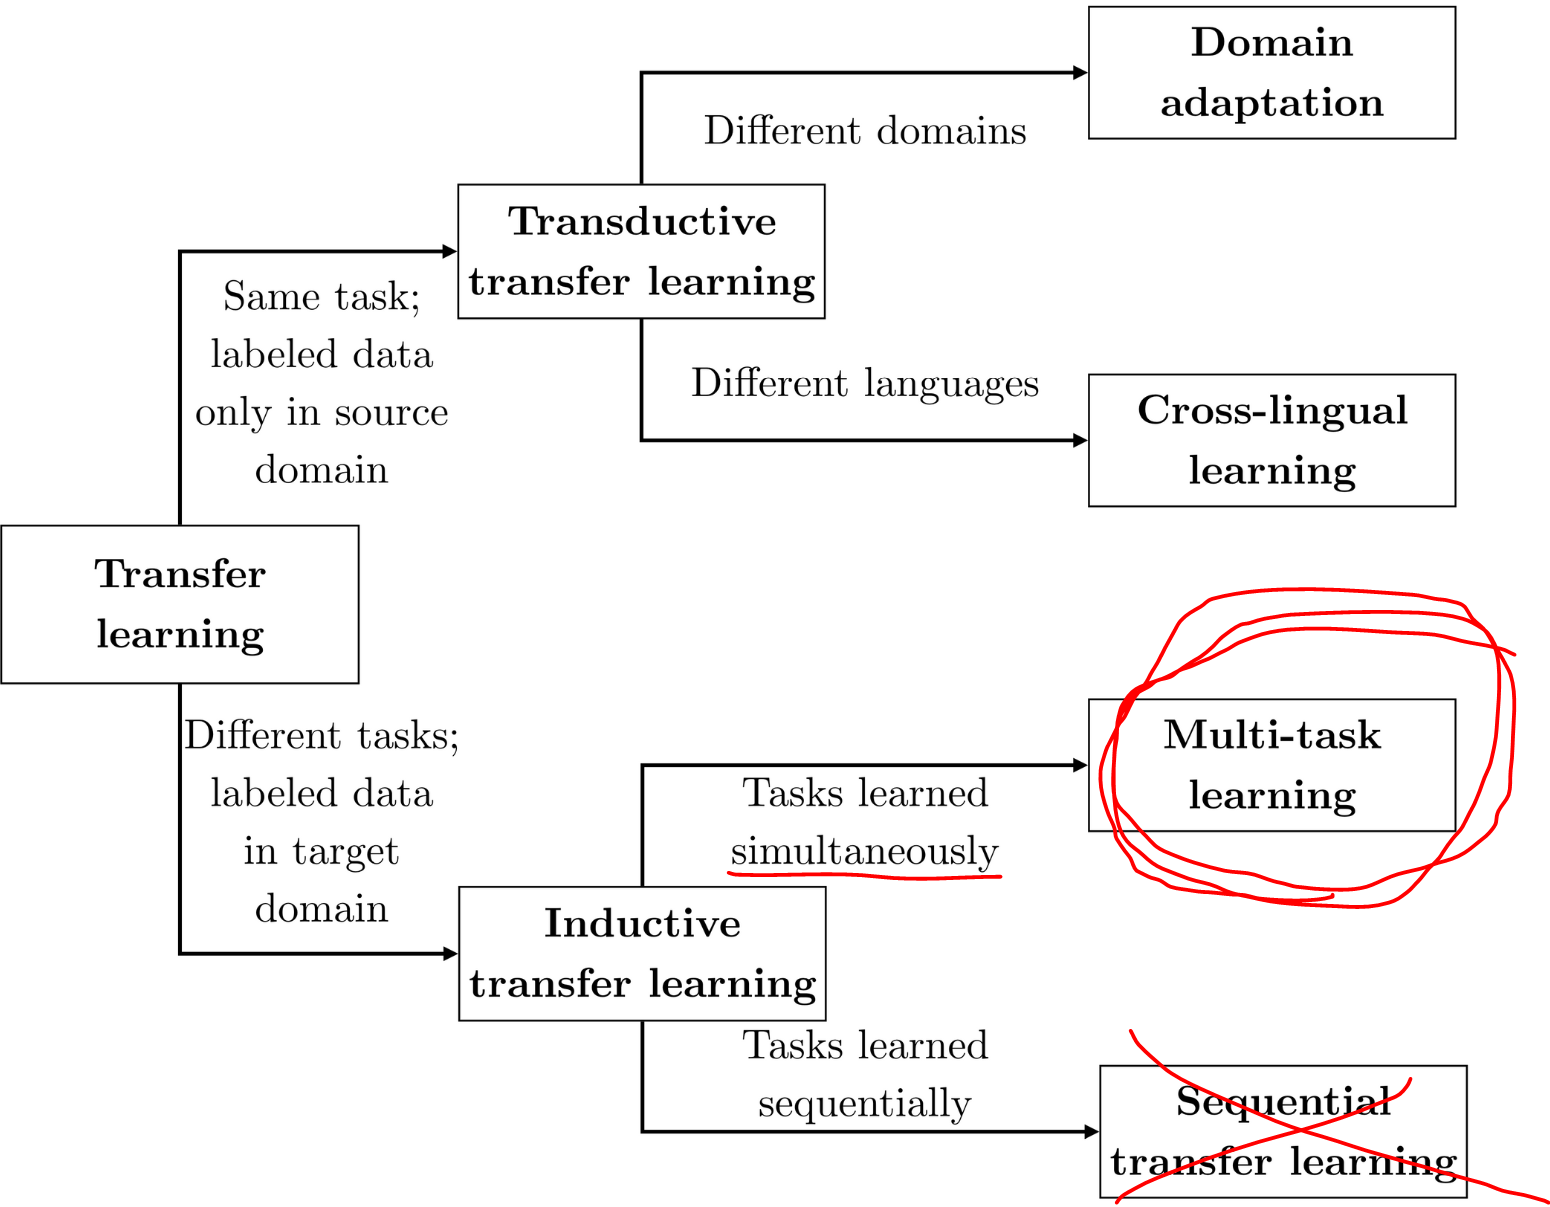
\includegraphics[width = 7cm]{figure/62-transfer_learning_taxonomy-anno.png}\\ 
	\beamergotobutton{Taxonomy of transfer learning \href{https://ruder.io/thesis/}{(Source: Ruder, 2019)}}
\end{figure}

\vfill

\end{frame}

% ------------------------------------------------------------------------------

\begin{frame}{multi-task learning?}

\vfill

\begin{itemize}
	\item \ques If the model can learn to link task descriptions to label sets, can it learn to perform multiple tasks at once?
	\item Yes, through fine tuning each task description$^1$ will be linked to its label set:
			\begin{itemize}
				\item \texttt{<task description a>} $\to$ \texttt{\{positive, negative\}}
				\item \texttt{<task description b>} $\to$ \texttt{\{world, sports, business, sci/tech\}} \citebutton{Example from AG News}{http://groups.di.unipi.it/~gulli/AG_corpus_of_news_articles.html}
				\item \texttt{<task description c>} $\to$ \texttt{\{spam, no spam\}}
				\item \texttt{<task description d>} $\to$ \texttt{\{entailment, contradiction, neutral\}}
			\end{itemize}
\end{itemize}

\vfill

$^1$\footnotesize{\texttt{<task description a>} (and so on) are just placeholders here.}
\end{frame}

% ------------------------------------------------------------------------------

\begin{frame}{multi-task learning?}

\vfill

\begin{itemize}
	\item \ques Can we have one single model for both different classification tasks \textbf{and} generation tasks?
			\begin{itemize}
				\item Yes, we just have to design suitable task descriptions
				\item Examples for \textit{generative} descriptions \citebutton{Raffel et al., 2020}{https://jmlr.org/papers/v21/20-074.html}
						\begin{itemize}
							\item \texttt{translate English to German: <input sample>}
							\item \texttt{summarize: <input sample>}
							\item \texttt{answer question: <input sample>}
						\end{itemize}
				\item Examples for \textit{classification} descriptions \citebutton{Raffel et al., 2020}{https://jmlr.org/papers/v21/20-074.html}
						\begin{itemize}
							\item \texttt{binary classification: <input sample>}
							\item \texttt{predict sentiment: <input sample>}
						\end{itemize}
			\end{itemize}
\end{itemize}

\vfill

\end{frame}

% ------------------------------------------------------------------------------

\begin{frame}{Text-to-Text Tasks}

\vfill
	
	\begin{figure}
		\centering
		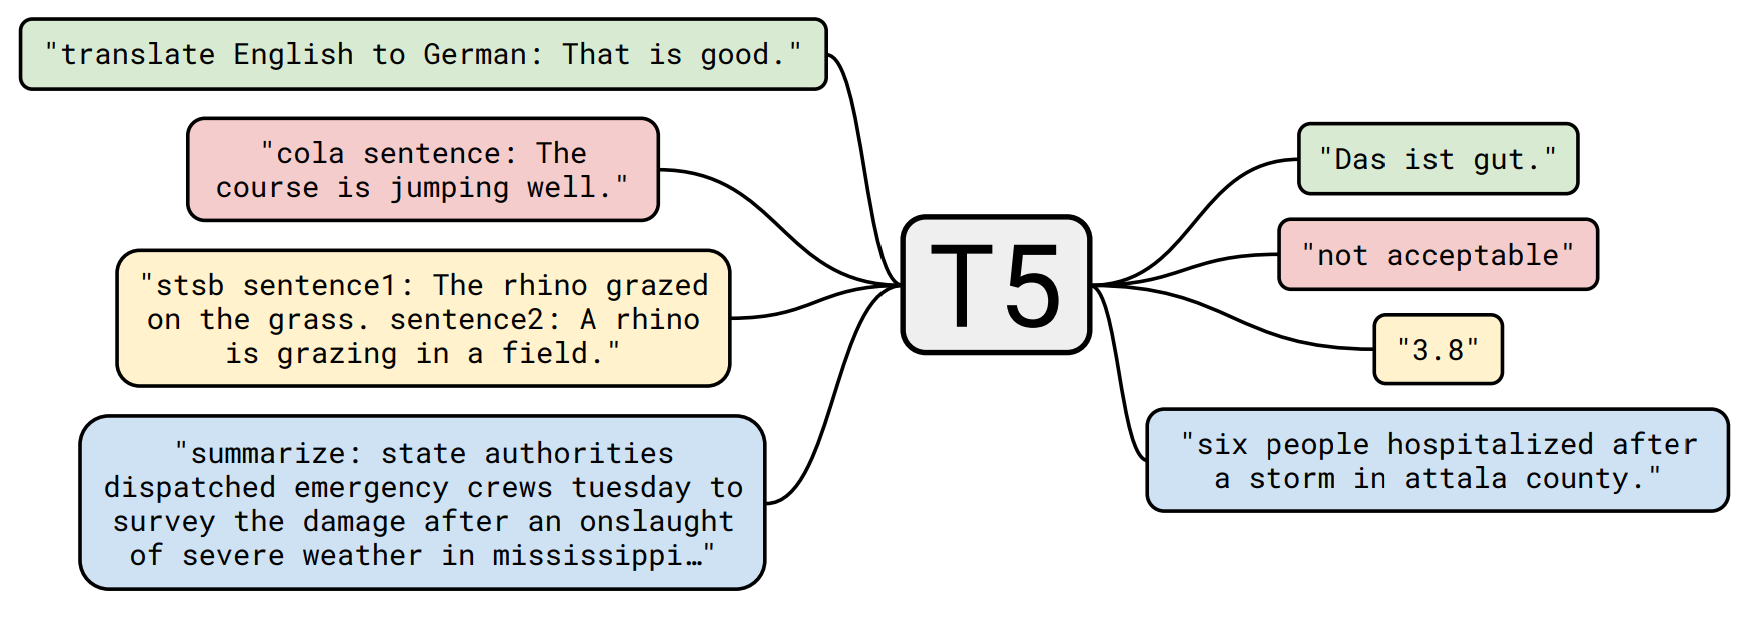
\includegraphics[width = 11cm]{figure/62-t5.png}\\ 
		\citebutton{Source: Raffel et al., 2020}{https://jmlr.org/papers/v21/20-074.html}
	\end{figure}
	
\begin{itemize}
	\item \textbf{Important note:} What we talked about as \texttt{<task description>} until now is commonly referred to as \texttt{<task prefix>}
\end{itemize}
	
\vfill

\end{frame}

% ------------------------------------------------------------------------------


%%%%%%%%%%%%%%%%%%%%%%%%%%%%%%%%%%%%%%%%%%%%%%%%%%%%%%%%%%%%%%%%%%
\section{Text-to-Text Transfer Transformer}
% Source: DL4NLP chapter06-post-bert-t5/slides-63-t5.tex
%%%%%%%%%%%%%%%%%%%%%%%%%%%%%%%%%%%%%%%%%%%%%%%%%%%%%%%%%%%%%%%%%%
% ------------------------------------------------------------------------------

\begin{frame}{Revisiting text-to-text tasks}

\vfill
	
	\begin{figure}
		\centering
		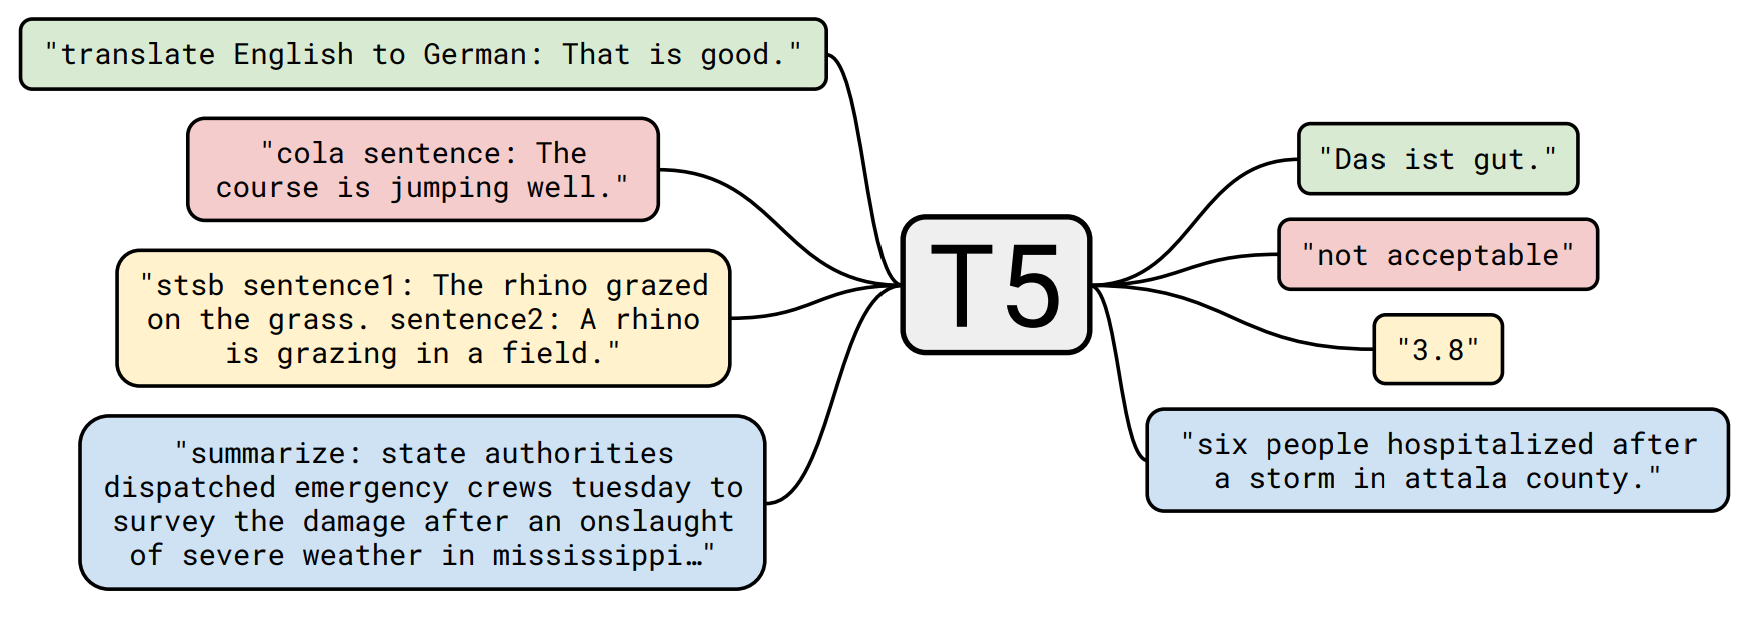
\includegraphics[width = 11cm]{figure/62-t5.png}\\ 
		\citebutton{Source: Raffel et al., 2020}{https://jmlr.org/papers/v21/20-074.html}
	\end{figure}
	
\textbf{Ingredients:}
	
\begin{itemize}
	\item \texttt{<task prefix>} for each task
	\item[] $\to$ Concatenation with the input
	\item Output label / score formatted as string
\end{itemize}
	
\vfill

\end{frame}

% ------------------------------------------------------------------------------

\begin{frame}{Text-to-Text Transfer Transformer}

\vfill

	\textbf{Short summary:}

	\begin{itemize}
		\item In short: T5 (bc of the five Ts)
		\item A complete encoder-decoder Transformer architecture
		\item[] \ques Why is this important?
		\item Relative positional embeddings
		\item All tasks reformulated as text-to-text tasks
		\item[] $\to$ Probably the most important innovation of this work
		\item From BERT-size $\times2$ (since enc-dec) up to 11B parameters
		\item Paradigm shift from \textit{Sequential Transfer Learning} towards true \textit{Multi-Task Learning}
	\end{itemize}
	
	\vspace{.5cm}

	\begin{center}
		\href{https://1.bp.blogspot.com/-o4oiOExxq1s/Xk26XPC3haI/AAAAAAAAFU8/NBlvOWB84L0PTYy9TzZBaLf6fwPGJTR0QCLcBGAsYHQ/s1600/image3.gif}{\textbf{\beamergotobutton{Nice Animation (similar to figure before)}}}
	\end{center}
	
\vfill

\end{frame}

% ------------------------------------------------------------------------------

\begin{frame}{input and output format}

\vfill

	\textbf{Input Side:}

	\begin{itemize}
		\item SentencePiece framework w/ WordPiece tokens
		\item Add task-specific (text) prefix to the original input
		\item Choice of the prefix: Hyperparameter!! 
		\item[$\to$] Changing this had limited impact
		\item[$\to$] No extensive experiments performed by the authors
	\end{itemize}
	
	\vspace{.5cm}

	\textbf{Output Side:}

	\begin{itemize}
		\item Output as a word or a piece of text (also numerical similarity scores)
		\item If output not present in set of potential alternatives, prediction considered as wrong (many other possible ways; this is not trivial)
	\end{itemize}
	
\vfill

\end{frame}

% ------------------------------------------------------------------------------

\begin{frame}{task prefix vs. prompting}

\vfill

	\textbf{Adding task-specific (text) prefix:}

	\begin{itemize}
		\item Add task-specific (text) prefix to the original input
		\item Model is fine-tuned on samples prepended with this prefix
		\item[$\to$] It learns to recognize what it is expected to do when encountering a specific prefix at test time
		\item[$\to$] Probably because of this: limited impact found by the authors
	\end{itemize}
	
	\vspace{.5cm}

	\textbf{Prompting:}

	\begin{itemize}
		\item Refers to just querying a trained w/o fine-tuning it (cf. next chapter)
		\item Paradigm of Few-/Zero-Shot Learning
		\item This is found to have a \textit{huge} impact on model performance
	\end{itemize}
	
\vfill

\end{frame}

% ------------------------------------------------------------------------------

\begin{frame}{architectural differences}

\vfill
	
	\textbf{Attention patterns (top) and Schematics of considered architectures (bottom)}
	
	\begin{figure}
		\centering
		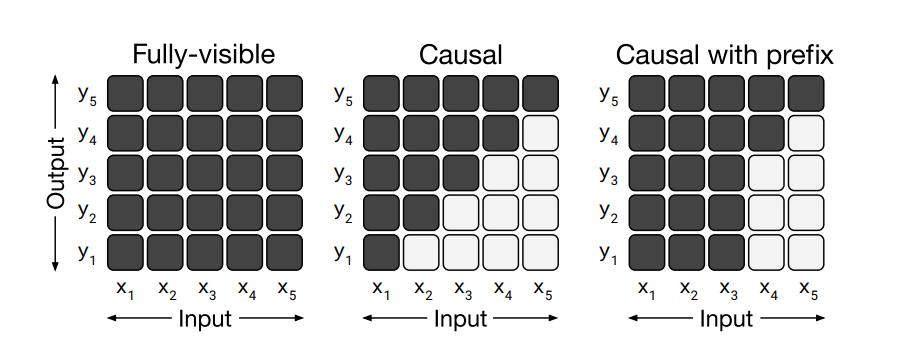
\includegraphics[width = 6.38cm]{figure/63-mask-patterns.png}\\ 
		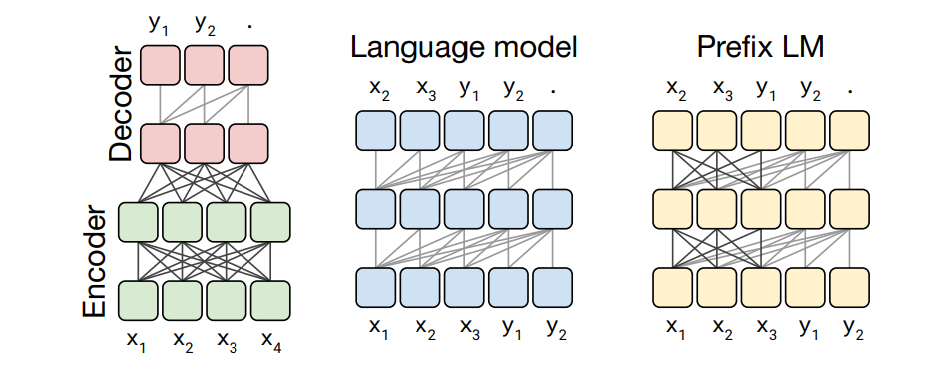
\includegraphics[width = 6.38cm]{figure/63-schematics.png}\\ 
		\citebutton{Source: Raffel et al., 2020}{https://jmlr.org/papers/v21/20-074.html}
	\end{figure}
	
\vfill

\end{frame}

% ------------------------------------------------------------------------------

\begin{frame}{pre-training objective}

\vfill
	
	\begin{figure}
		\centering
		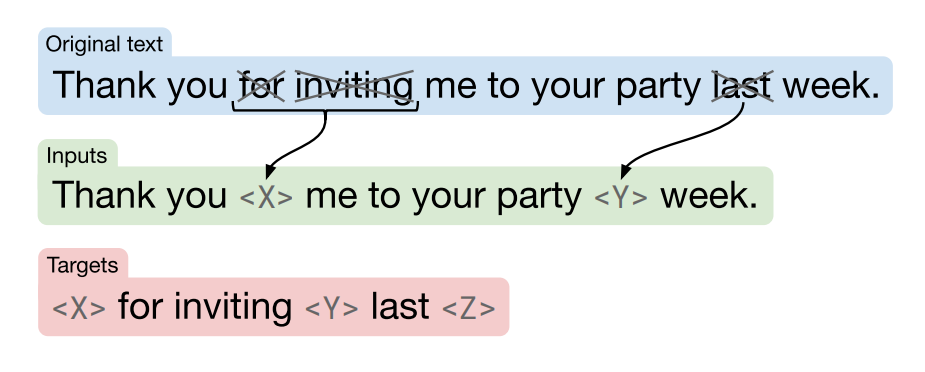
\includegraphics[width = 11cm]{figure/63-t5-span-pred.png}\\ 
		\citebutton{Source: Raffel et al., 2020}{https://jmlr.org/papers/v21/20-074.html}
	\end{figure}
	
	\begin{enumerate}
		\item Mark spans in input sequence for corruptions
		\item Replace tokens with sentinel tokens
		\item Predict sentinel tokens and replaced tokens
	\end{enumerate}
	
\vfill

\end{frame}

% ------------------------------------------------------------------------------

\begin{frame}{Pre-training objectives}

\vfill

	\begin{itemize}
		\item Authors experimented with different objectives
		\item Most of them rely in some way on MLM
	\end{itemize}
	
	\begin{figure}
		\centering
		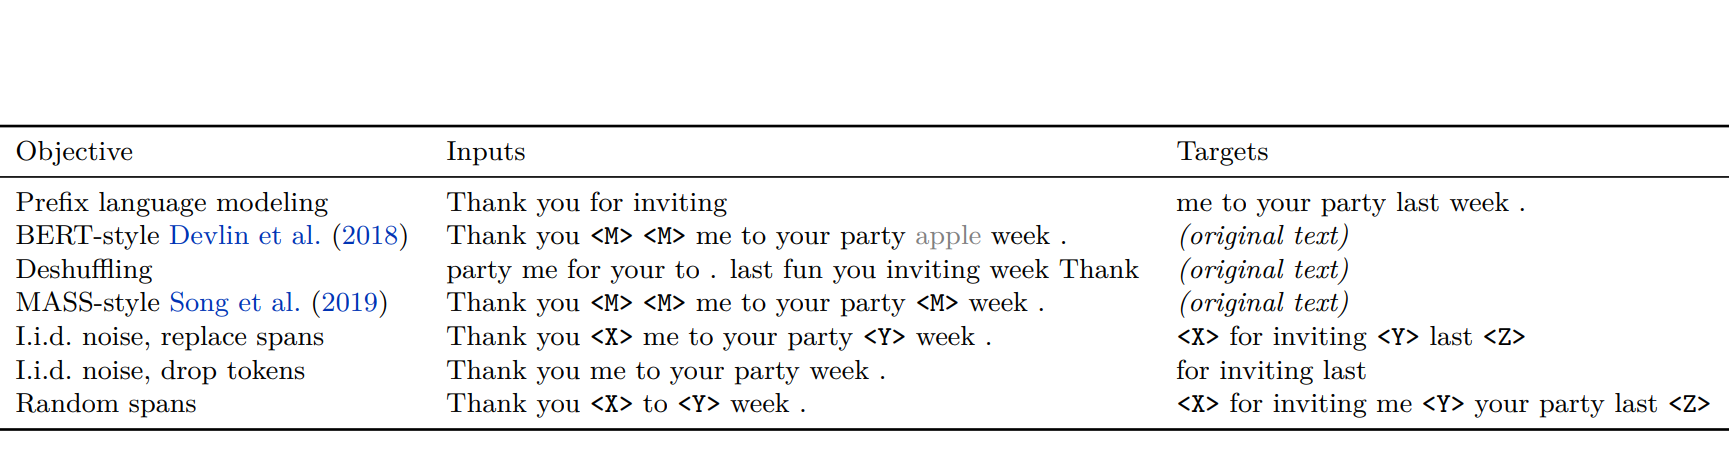
\includegraphics[width = 11cm]{figure/63-t5-objectives1.png}\\ 
		\citebutton{Source: Raffel et al., 2020}{https://jmlr.org/papers/v21/20-074.html}
	\end{figure}
	
\vfill

\end{frame}

% ------------------------------------------------------------------------------

\begin{frame}{Pre-training objectives}

\vfill

	\begin{figure}
		\centering
		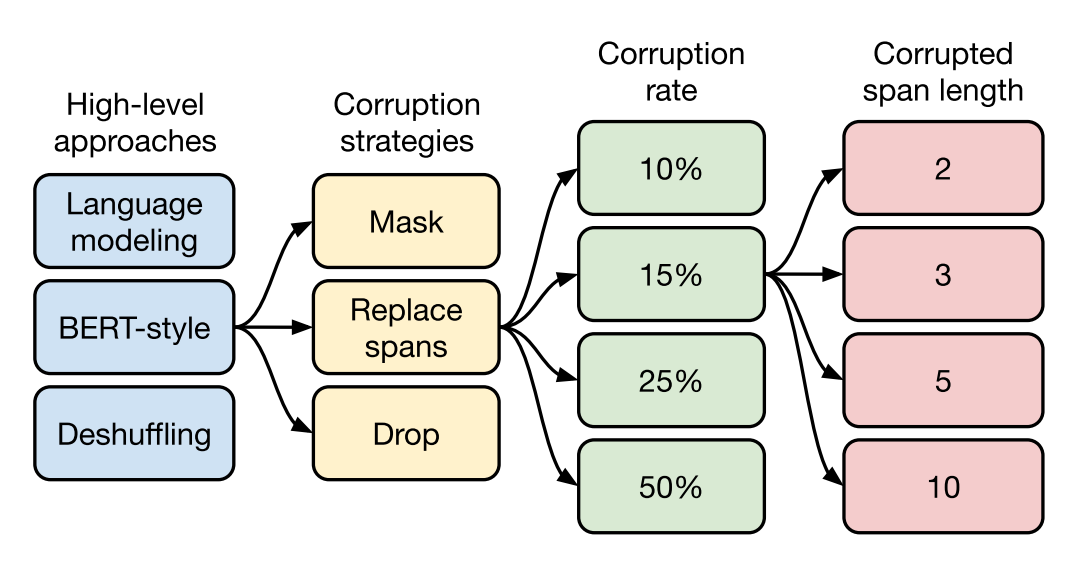
\includegraphics[width = 11cm]{figure/63-t5-objectives2.png}\\ 
		\citebutton{Source: Raffel et al., 2020}{https://jmlr.org/papers/v21/20-074.html}
	\end{figure}
	
\vfill

\end{frame}

% ------------------------------------------------------------------------------

\begin{frame}{The \textbf{C}olossal \textbf{C}lean \textbf{C}rawled \textbf{C}orpus (C4)}

\vfill

	\begin{itemize}
		\item Effort to measure the effect of quality, characteristics \& size of the pre-training resources
		\item Common Crawl as basis, careful cleaning and filtering for English language
		\item Orders of magnitude larger (750GB) compared to commonly used corpora 
	\end{itemize}
	
\vfill

\end{frame}

% ------------------------------------------------------------------------------

\begin{frame}{The \textbf{C}olossal \textbf{C}lean \textbf{C}rawled \textbf{C}orpus (C4)}

\vfill
	
	\textbf{Experiments (with respect to C4)}
	
	\begin{figure}
		\centering
		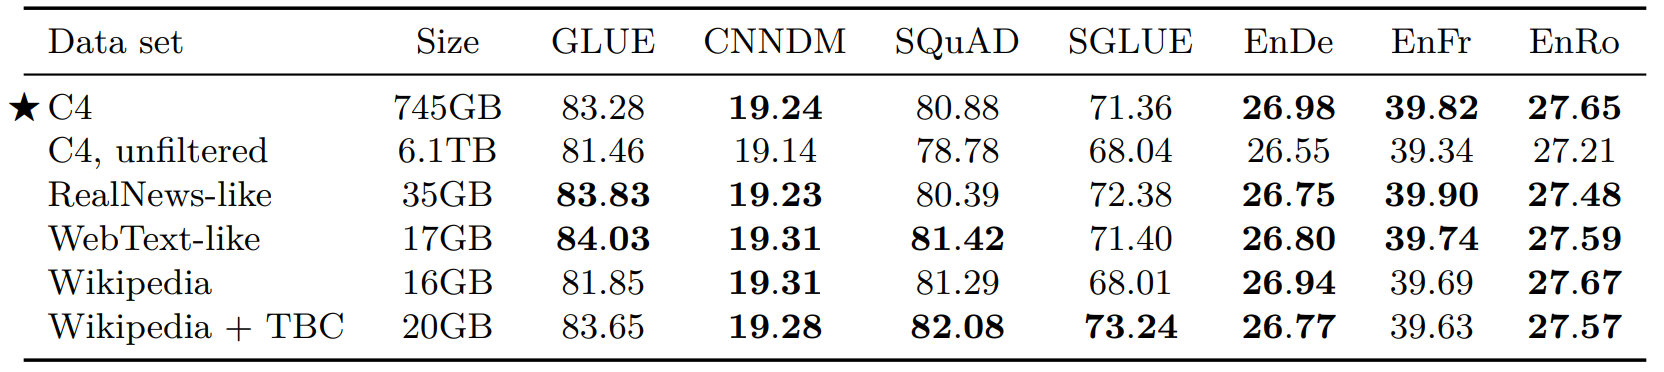
\includegraphics[width = 9cm]{figure/63-c4-characteristics.png}\\ 
		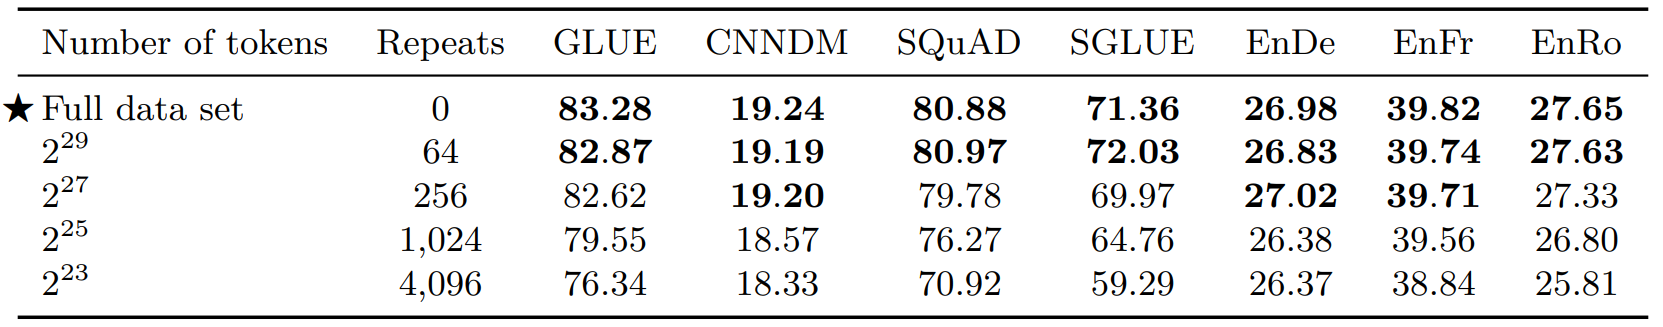
\includegraphics[width = 9cm]{figure/63-c4-size.png}\\ 
		\citebutton{Source: Raffel et al., 2020}{https://jmlr.org/papers/v21/20-074.html}
	\end{figure}
	
\vfill

\end{frame}

% ------------------------------------------------------------------------------

\begin{frame}{T5 - Exhaustive Experiments}

\vfill

	\textbf{Performed experiments with respect to ..}
	
	\begin{itemize}
		\item \textit{.. architecture, size \& objective}
		\item[$\to$] enc, dec, enc-dec
		\item[$\to$] Between 60M and 11B parameters
		\item \textit{.. details of the Denoising objective (which was found to work best)}
		\item \textit{.. fine-tuning methods}
		\item[$\to$] Adapter layers
		\item[$\to$] Gradual Unfreezing (cf. ULMFiT)
		\item \textit{.. Multi-task learning strategies}
		\item[$\to$] Examples-proportional mixing
		\item[$\to$] Temperature-scaled mixing
	\end{itemize}
	
\vfill

\end{frame}

% ------------------------------------------------------------------------------

\begin{frame}{Benchmark results}

\vfill

	\begin{figure}
		\centering
		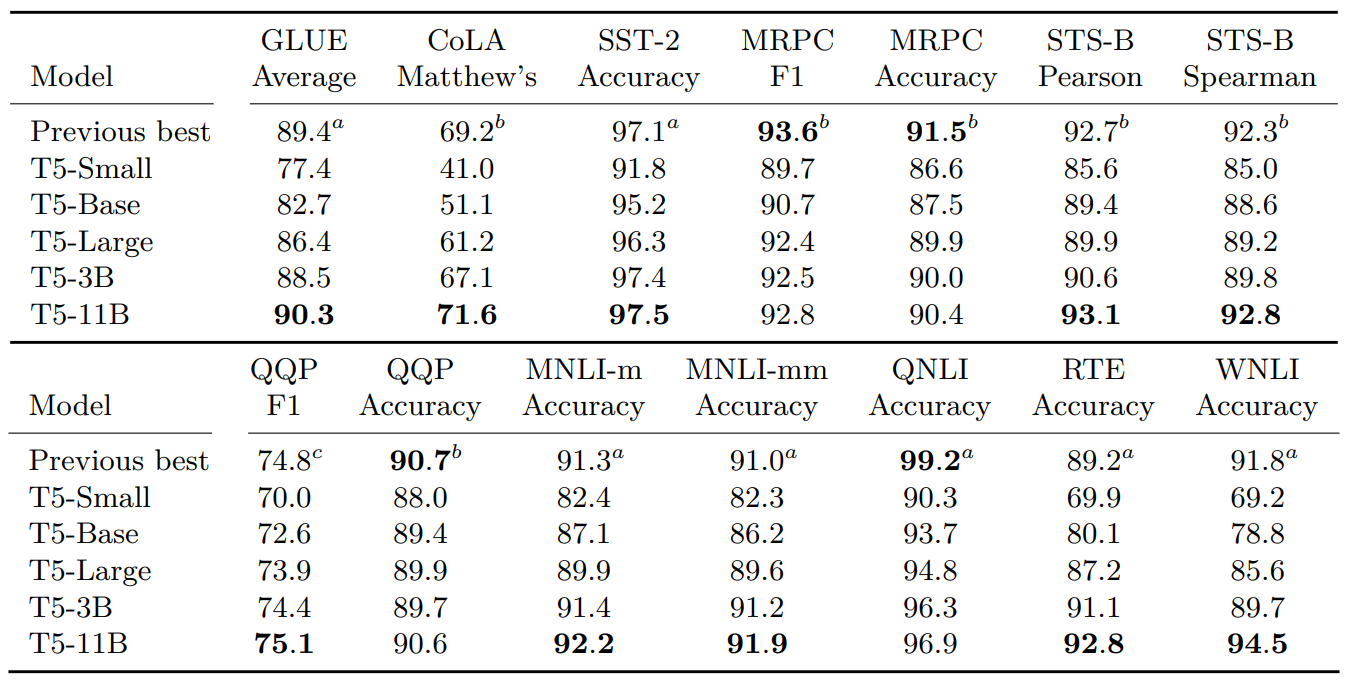
\includegraphics[width = 9cm]{figure/63-t5-glue.png}\\ 
		\citebutton{Source: Raffel et al., 2020}{https://jmlr.org/papers/v21/20-074.html}
	\end{figure}
	
\vfill

\end{frame}

% ------------------------------------------------------------------------------

\begin{frame}{Benchmark results}

\vfill

	\begin{figure}
		\centering
		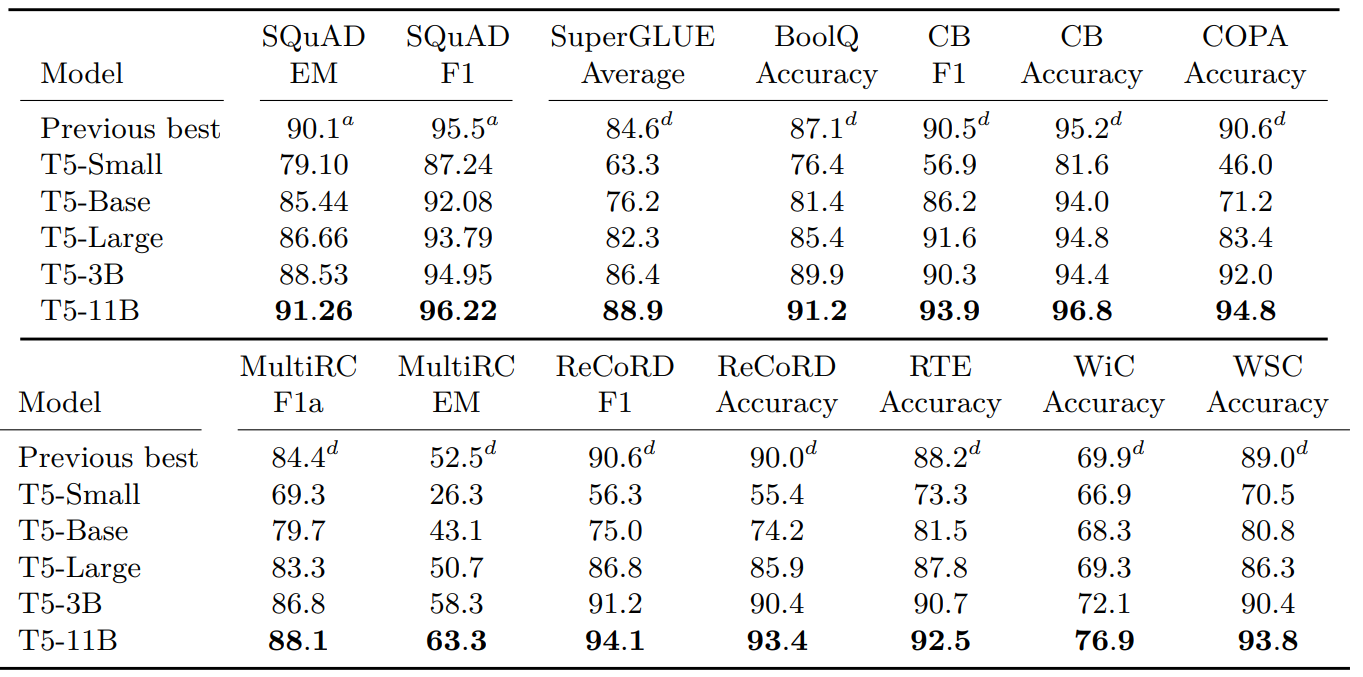
\includegraphics[width = 9cm]{figure/63-t5-squad-sglue.png}\\ 
		\citebutton{Source: Raffel et al., 2020}{https://jmlr.org/papers/v21/20-074.html}
	\end{figure}
	
\vfill

\end{frame}

% ------------------------------------------------------------------------------

\begin{frame}{Benchmark results}

\vfill

	\begin{figure}
		\centering
		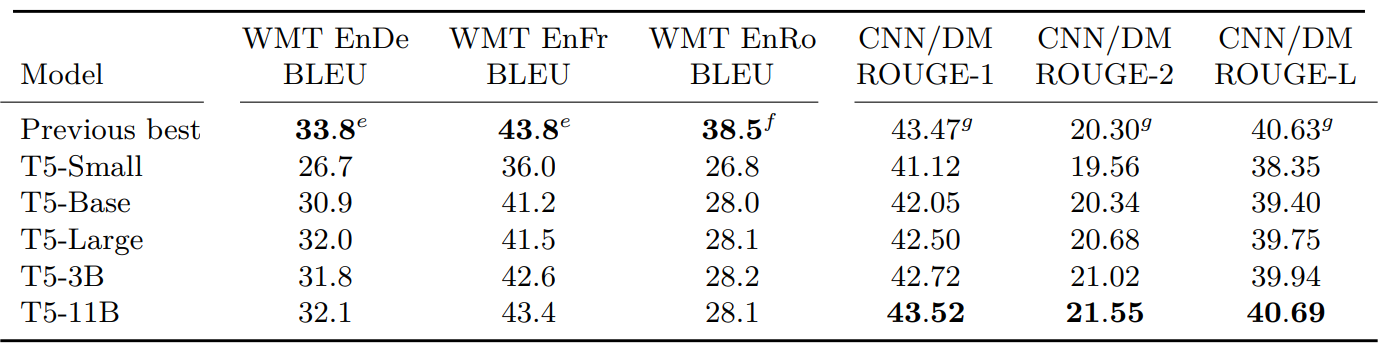
\includegraphics[width = 9cm]{figure/63-t5-mt.png}\\ 
		\citebutton{Source: Raffel et al., 2020}{https://jmlr.org/papers/v21/20-074.html}
	\end{figure}
	
\vfill

\end{frame}

% ------------------------------------------------------------------------------

\begin{frame}{T5 - Exhaustive Experiments}

\vfill
	
	\textbf{Conclusions}
	
	\begin{itemize}
		\item Encoder-decoder architecture works best in this "text-to-text" setting
		\item More data, larger models \& ensembling all boost the performance
			\begin{itemize}
				\item Larger models trained for fewer steps better than smaller models on more data
				\item Ensembling: Using same base pre-trained models worse than complete separate model ensembles
			\end{itemize}
		\item Different denoising objectives work similarly well
		\item Updating \textit{all} model parameters during fine-tuning works best (but expensive)
	\end{itemize}
	
\vfill

\end{frame}

% ------------------------------------------------------------------------------

\begin{frame}{Different T5 versions}
\textit{Similar to BERT T5 has different versions, which all have a different parameter count} \citebutton{Raffel et al., 2020}{https://arxiv.org/abs/1910.10683}

\begin{table}[h!]
\centering
\small % Reduce font size
\begin{tabular}{|c|c|c|c|c|c|c|}
\hline
\textbf{Model} & \textbf{Parameters} & $\bm{n_{layers}}$ & $\bm{d_{model}}$ & $\bm{d_{FFN}}$ & $\bm{d_{qkv}}$ & $\bm{n_{heads}}$ \\ \hline
small  & 60M  & 6  & 512  & 2048 & 64 & 8 \\ \hline
base   & 220M & 12 & 768  & 3072 & 64 & 12 \\ \hline
large  & 770M & 24 & 1024 & 4096 & 64 & 16 \\ \hline
3B     & 3B   & 24 & 1024 & 16384 & 128 & 32 \\ \hline
11B    & 11B  & 24 & 1024 & 65536 & 128 & 128 \\ \hline
\end{tabular}
\end{table}

\begin{itemize}
    \item For T5 small, base and large we have the following parameter count per encoder/decoder layer:
    \begin{itemize}
        \item $N_{Encoder} = 12\cdot d_{model}^2$
        \item $N_{Decoder} = 16\cdot d_{model}^2$
    \end{itemize}
		\item \textit{For T5 3B and 11B $N_{Encoder}$ and $N_{Decoder}$ are different!}
\end{itemize}
    
\end{frame}



%-------------------------------------------------------------------------------

\begin{frame}{Approximate Parameter Count (1)}
\textit{The general formula is:} $$N_{Total} = n_{layers}\cdot (N_{Encoder} + N_{Decoder}) + N_{Embedding}$$

\begin{itemize}
    \item Let $V = 32000$ be the size of the vocabulary, we then have: $$N_{Embedding} = 32000 \times d_{model}$$

    \item \textbf{T5 small}:
        $$N_{small} = 6\cdot (12\cdot 512^2 + 16\cdot 512^2) + 32000\times 512 = 60,424,192$$
    \item \textbf{T5 base}:
        $$N_{base} = 12\cdot (12\cdot 768^2 + 16\cdot 768^2) + 32000\times 768 = 222,756,864$$
    \item \textbf{T5 large}:
        $$N_{large} = 24\cdot (12\cdot 1024^2 + 16\cdot 1024^2) + 32000\times 1024 = 737,411,072$$
    
\end{itemize}
    
\end{frame}

%-------------------------------------------------------------------------------

\begin{frame}{Revisiting: MHA and FFN (1)}

\begin{itemize}
    \item In the transformer chapter we derived the FFN parameter count to be $\bm{8\cdot d_{model}}$
    \item We also derived the MHA parameter count to be $\bm{4\cdot d_{model^2}}$ 
    \item But this is only the case if we choose $d_{FFN} = 4\cdot d_{model}$ and $d_{qkv} = \frac{d_{model}}{n_{heads}}$, with $d_{FFN}$ being the hidden dimension of the FFN and $d_{qkv}$ being the embedding dimension of each head in MHA 
    \item For the two bigger model variants we have the following relations:
    \begin{itemize}
        \item \textbf{T5 3B}: $d_{FFN} = 16\cdot d_{model}$ and $d_{qkv} \neq \frac{d_{model}}{n_{heads}}$
        \item \textbf{T5 11B}: $d_{FFN} = 64\cdot d_{model}$ and $d_{qkv} \neq \frac{d_{model}}{n_{heads}}$ 
    \end{itemize}
    \item Thats why we can't use the same formulas as for the three previous variants
\end{itemize}
    
\end{frame}

%-------------------------------------------------------------------------------

\begin{frame}{Revisiting: MHA and FFN (2)}

\begin{itemize}
    \item In MHA $n_{heads} \cdot d_{qkv}$ is no longer $d_{model}$:
		
					\begin{align*}
					N_{attention} &= n_{heads} \cdot d_{qkv} \times d_{model} + (d_{model} \times d_{qkv}) \times n_{heads} \cdot 3 \\
					&= 4\cdot n_{heads}\cdot d_{qkv} \times d_{model}\text{;}\quad \text{instead of:}\quad 4\cdot d_{model}^2
					\end{align*}
    
    \item For the FFN $d_{FFN}$ is no longer $4\cdot d_{model}$:

					\begin{align*}
					N_{FFN} &= d_{model} \times d_{FFN} + d_{FFN} \times d_{model} \\
					&= 2\cdot d_{model} \times d_{FFN}\text{;}\quad \text{instead of:}\quad 8\cdot d_{model}^2
					\end{align*}

    \item For the Encoder and Decoder that means:
    \begin{itemize}
        \item $N_{Encoder} = 4\cdot n_{heads}\cdot d_{qkv} \times d_{model} + 2\cdot d_{model} \times d_{FFN}$
        \item $N_{Decoder} = 2\cdot 4\cdot n_{heads}\cdot d_{qkv} \times d_{model} + 2\cdot d_{model} \times d_{FFN} $
    \end{itemize}

\end{itemize}
    
\end{frame}

%-------------------------------------------------------------------------------

\begin{frame}{Approximate Parameter Count (2)}
\small% fit16:9

\textit{The general formula is still:} $$N_{Total} = n_{layers}\cdot (N_{Encoder} + N_{Decoder}) + N_{Embedding}$$

\begin{itemize}
    \item \textbf{T5 3B}: 

					\begin{align*}
							N_{3B} &= 24\cdot ([4\cdot 32\cdot 128 \times 1024 + 2\cdot 1024 \times 16384] \\
							&+ [2\cdot 4 \cdot 32\cdot 128 \times 1024 + 2\cdot 1024 \times 16384]) + 32000\cdot 1024 \\
							&= 2,851,340,288 \approx 3B
					\end{align*}

    \item \textbf{T5 11B}:

					\begin{align*}
							N_{11B} &= 24\cdot ([4\cdot 128\cdot 128 \times 1024 + 2\cdot 1024 \times 65536] \\
							&+ [2\cdot 4 \cdot 128\cdot 128 \times 1024 + 2\cdot 1024 \times 65536]) + 32000\cdot 1024 \\
							&= 11,307,057,152 \approx 11B
					\end{align*}

\end{itemize}
    
\end{frame}

%-------------------------------------------------------------------------------


%%%%%%%%%%%%%%%%%%%%%%%%%%%%%%%%%%%%%%%%%%%%%%%%%%%%%%%%%%%%%%%%%%
\section{License \& Attribution}
%%%%%%%%%%%%%%%%%%%%%%%%%%%%%%%%%%%%%%%%%%%%%%%%%%%%%%%%%%%%%%%%%%

\begin{vbframe}{License \& Attribution}
\begin{itemize}
\item \textbf{Single source.} All content is taken from \textbf{Deep Learning for NLP (DL4NLP)}, SLDS, LMU Munich, chapters 4 (\textit{BERT}), 5 (\textit{Post-BERT Era: BERT-based}) and 6 (\textit{Post-BERT Era: T5}), in the source's own order --- licensed \textbf{CC BY 4.0}: \url{https://creativecommons.org/licenses/by/4.0/}.
\item Figures are reproduced as they appear in DL4NLP, with the attributions DL4NLP itself gives (several are credited there to the original papers or to Jay Alammar's \textit{The Illustrated BERT}).
\end{itemize}
\end{vbframe}

\endlecture
\end{document}
